\anachapter{Notions élémentaires à usage dans les batteries}
\label{chp:notions_elementaires}


\objectif{

\faBattery[0] Concepts d'oxydo-réduction
\begin{itemize}[label=\faAngleRight]
    \item pile vs accumulateur \& batterie primaire vs secondaire ;
    \item oxydant vs réducteur \& oxydation vs réduction ;
    \item anode vs cathode \& conventions générateur/récepteur ;
    \item potentiel électrique \& potentiel d'électrode ;
    \item tension à courant nul \& force électromotrice ;
    \item composantes d'une cellule : électrodes, électrolyte, séparateur.
\end{itemize}

\faBattery[2] Chimie des batteries
\begin{itemize}[label=\faAngleRight]
	\item réaction de recomposition : formation, déplacement ;
	\item réaction d'insertion : insertion, intercalation, extrusion, topotacticité vs atacticité.
\end{itemize}

\faBattery[4] Connaître les caractéristiques sur l'état ou les performances d'une batterie
\begin{itemize}[label=\faAngleRight]
    \item courant, tension, puissance électrique ;
    \item état de charge et décharge ;
	\item capacité spécifique massique et volumique ;
	\item état de santé ;
	\item énergie théorique maximale ;
	\item qualité énergétique ;
	\item cyclabilité.
\end{itemize}}

\begin{figure}[H]
\centering
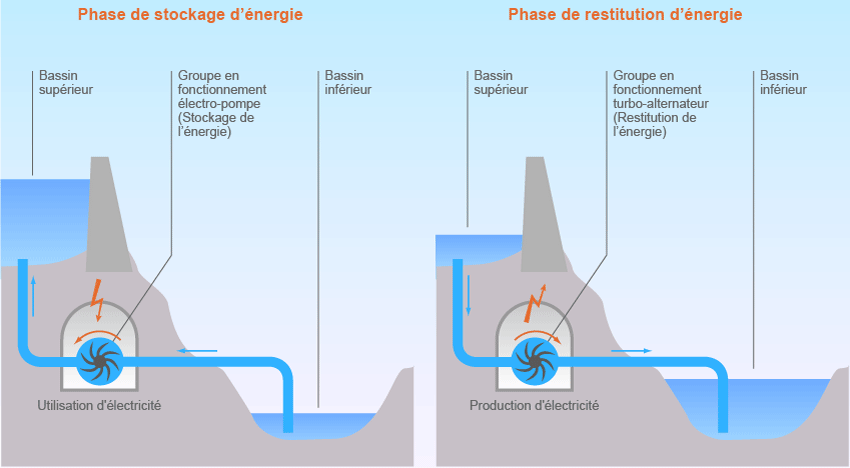
\includegraphics[width=\textwidth]{figures-Chp0/Fig15}
\captionof{figure}{Principe de fonctionnement d'une centrale STEP (Station de Transfert d'\'{E}nergie par Pompage)}
\label{fig:Chp-0-15}
\end{figure}
%https://www.encyclopedie-energie.org/les-stations-de-pompage-step/

Une batterie est un dispositif qui stocke de l'énergie sous forme \blancbis{chimique} et qui le restitue sous forme d'énergie \blancbis{électrique}. En ce sens, on qualifie une batterie de \blancbis{transducteur}\mySideNote{Terme associé à tout dispositif permettant la conversion d'une grandeur physique en une autre.} ou de \blancbis{convertisseur d'énergie}.

De manière assez simple, il est possible d'établir une analogie avec la mécanique. Les stations de transfert d'énergie par pompage, représentées à la Fig. \ref{fig:Chp-0-15}, sont un bon exemple modèle. Lorsque le réseau électrique est en déficit d'énergie électrique, ces stations de haute montagne déversent l'eau du bassin supérieur vers le bassin inférieur. Cette phase correspond à la phase de "décharge" du bassin, où l'énergie potentielle de pesanteur est convertie en énergie électrique. Dans le cas où le réseau est excedentaire en énergie, l'eau du bassin est remontée par un système de pompe. La STEP convertit donc l'énergie électrique en énergie potentielle de pesanteur.


Dans une batterie, un opérateur va mettre en contact deux électrodes\mySideNote{Conducteur électronique (\emph{par ex.} un métal) ou ionique (\emph{par ex.} le verre) captant ou libérant des électrons} où les électrons ont une énergie chimique différente. Lors de cette mise en contact, cette différence d'énergie chimique conduit à la mise en mouvement d'un flux d'électron\mySideNote{Ce flux se manifeste par un courant électrique, noté $I$, qui représente la quantité de charge transporté à travers un conducteur par unité de temps.}. Le flux d'électron conduit petit à petit à un retour à l'équilibre du système.

Lors de ce processus, \blancbis{deux espèces chimiques rédox}, c'est-à-dire des espèces chimiques capables d'\blancbis{échanger un ou plusieurs électrons}, réagissent ensemble. Cette réaction libère de l'énergie sous deux formes : 
\begin{itemize}
    \item un \blancbis{travail utile} \textbf{W'} qui est le travail électrique ;
    \item une \blancbis{déperdition d'énergie}, la chaleur \textbf{Q}, c'est-à-dire de l'énergie thermique.
\end{itemize}

\begin{minipage}[c]{0.65\textwidth}
\centering
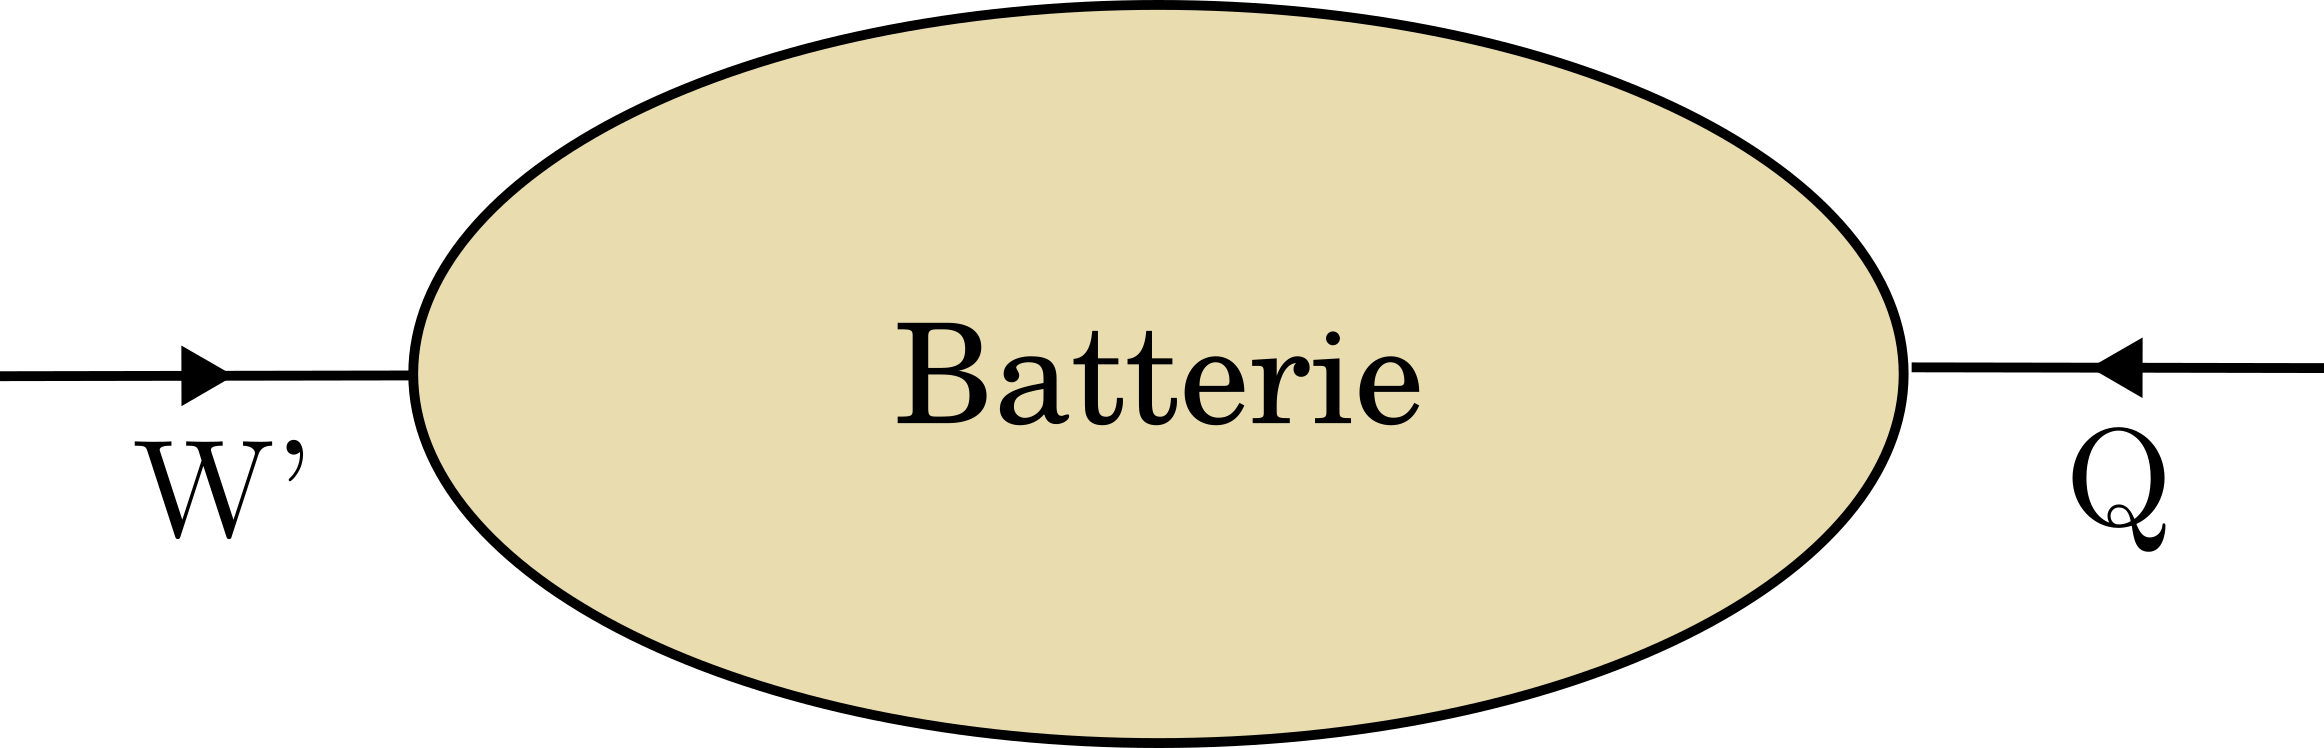
\includegraphics[width=5cm]{figures-Chp0/Fig02.png}
\end{minipage}\hfill   
\begin{minipage}[c]{0.35\textwidth}     
\captionof{figure}{Représentation des flux d'énergie reçus par une batterie.}
\label{fig:Chp-0-02}
\end{minipage}

La batterie est parfois à usage unique ou rechargeable. Ainsi, si la batterie est rechargeable, le travail électrique est soit reçu $W' > 0$ (charge) ou cédé $W' < 0$ (décharge). En son sein, des éléments résistifs imposent que la batterie perd nécessairement, que ça soit en charge ou décharge, une partie de son énergie sous forme thermique $Q < 0$.\mySideNote{\centering
\begin{tabular}{ccc}
& Charge & Décharge \\
$W'$ & $> 0$ & $< 0$\\
$Q$ & $< 0$ & $< 0$ \\
\end{tabular}}

Cette capacité à recevoir ou non du travail électrique permet de classifier les batteries en plusieurs catégories.

\section{Classification des générateurs électrochimiques}

\subsection{Dispositif constitué d'une seule cellule électrochimique}

\begin{figure}[H]
\begin{center}
\begin{tabular}{cc}
\subfloat[\label{fig:03a}]{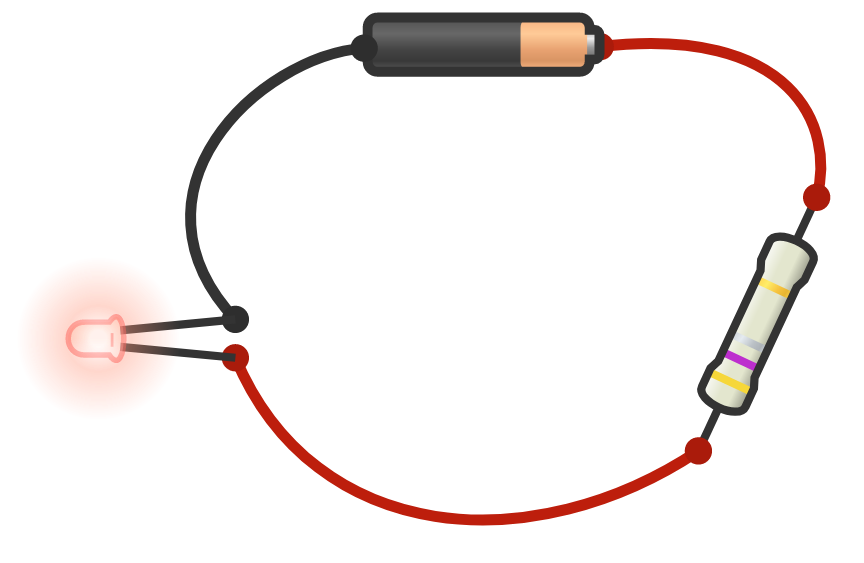
\includegraphics[width=3cm]{figures-Chp0/Fig03a}} & \subfloat[\label{fig:03c}]{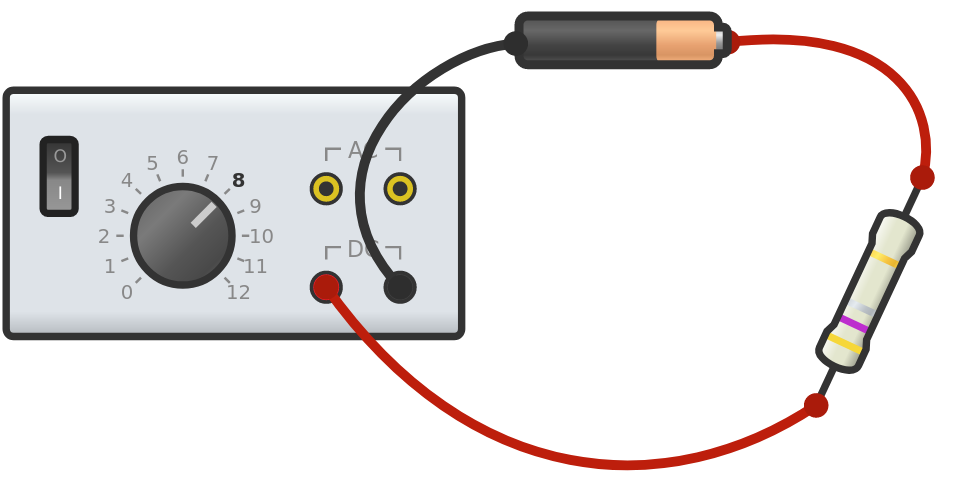
\includegraphics[width=3cm]{figures-Chp0/Fig03c}} \\
\subfloat[\label{fig:03b}]{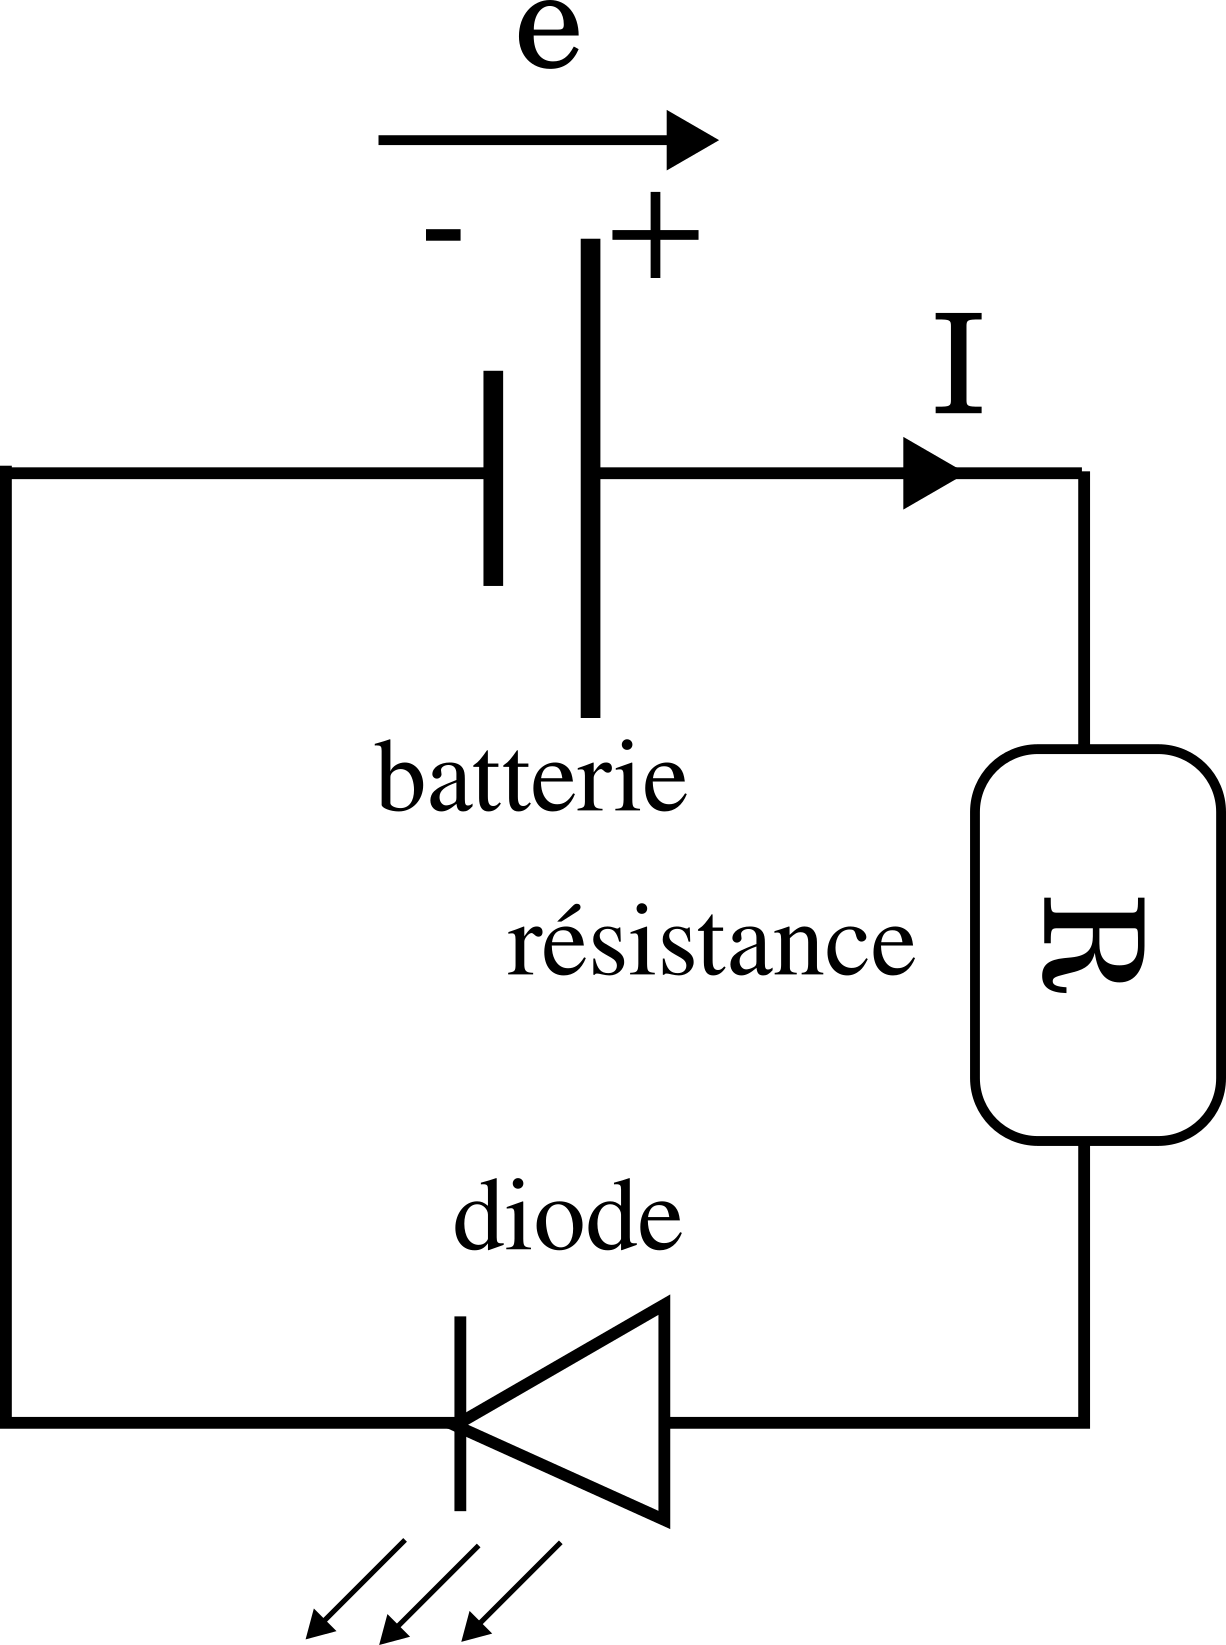
\includegraphics[width=3cm]{figures-Chp0/Fig03b}} & \subfloat[\label{fig:03d}]{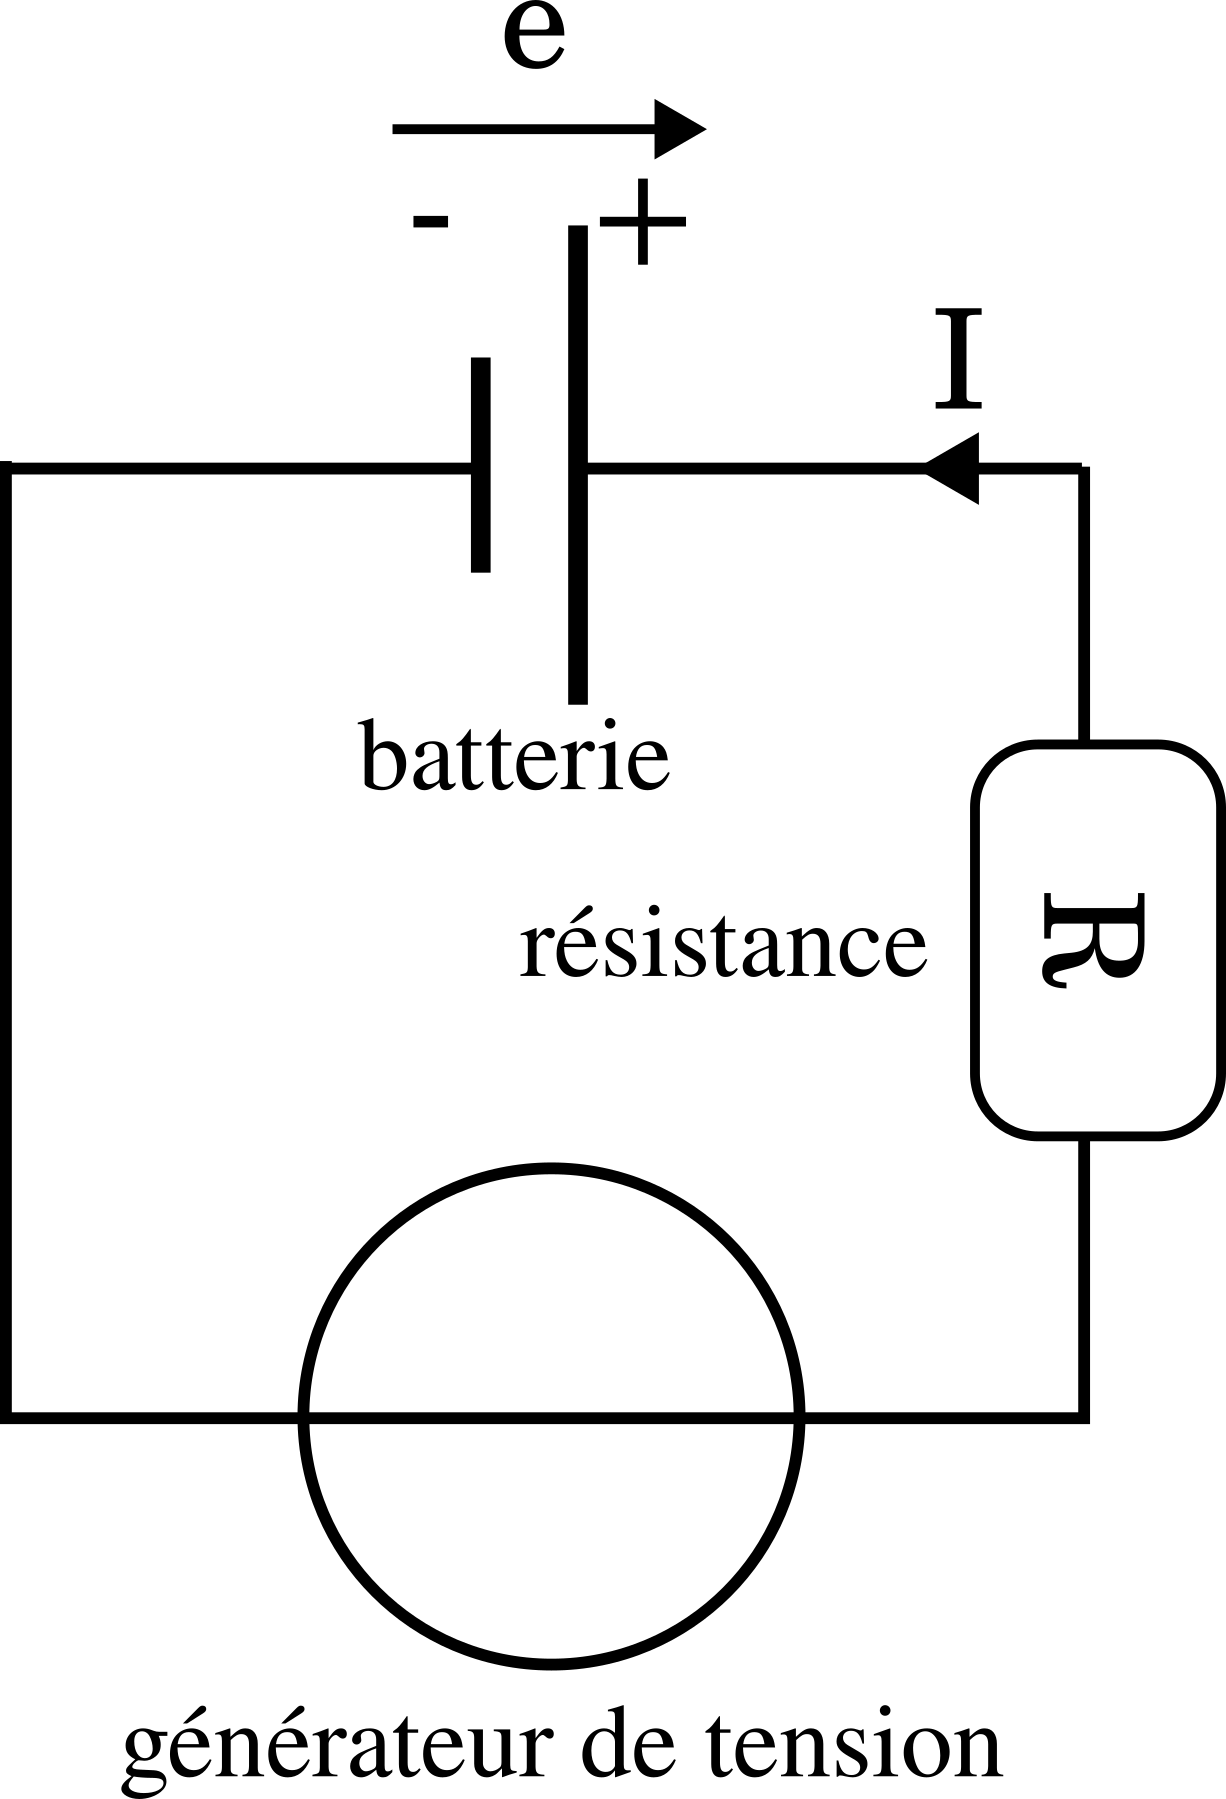
\includegraphics[width=3cm]{figures-Chp0/Fig03d}}
\end{tabular}
\end{center}

%\begin{centering}
%\subfloat[\label{fig:03a}]{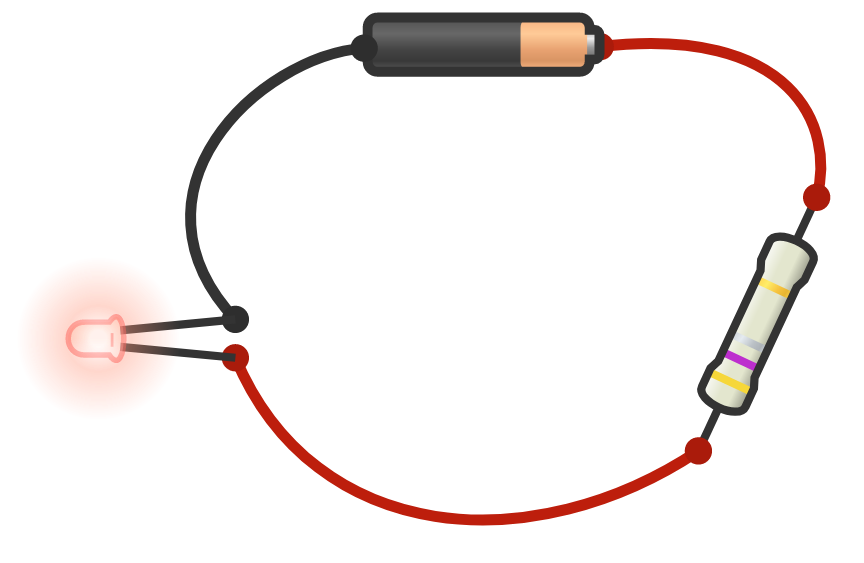
\includegraphics[height=3cm]{figures-Chp0/Fig03a}}\subfloat[\label{fig:03c}]{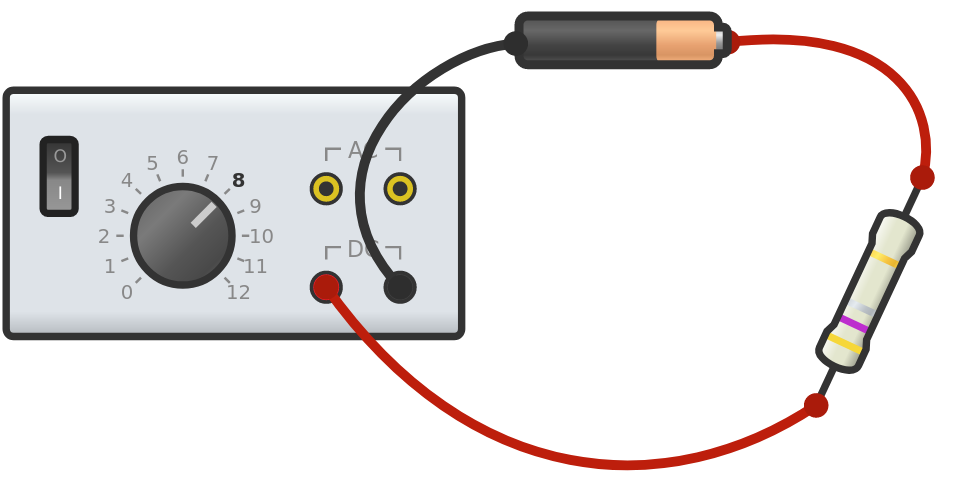
\includegraphics[height=3cm]{figures-Chp0/Fig03c}}\hfill\subfloat[\label{fig:03b}]{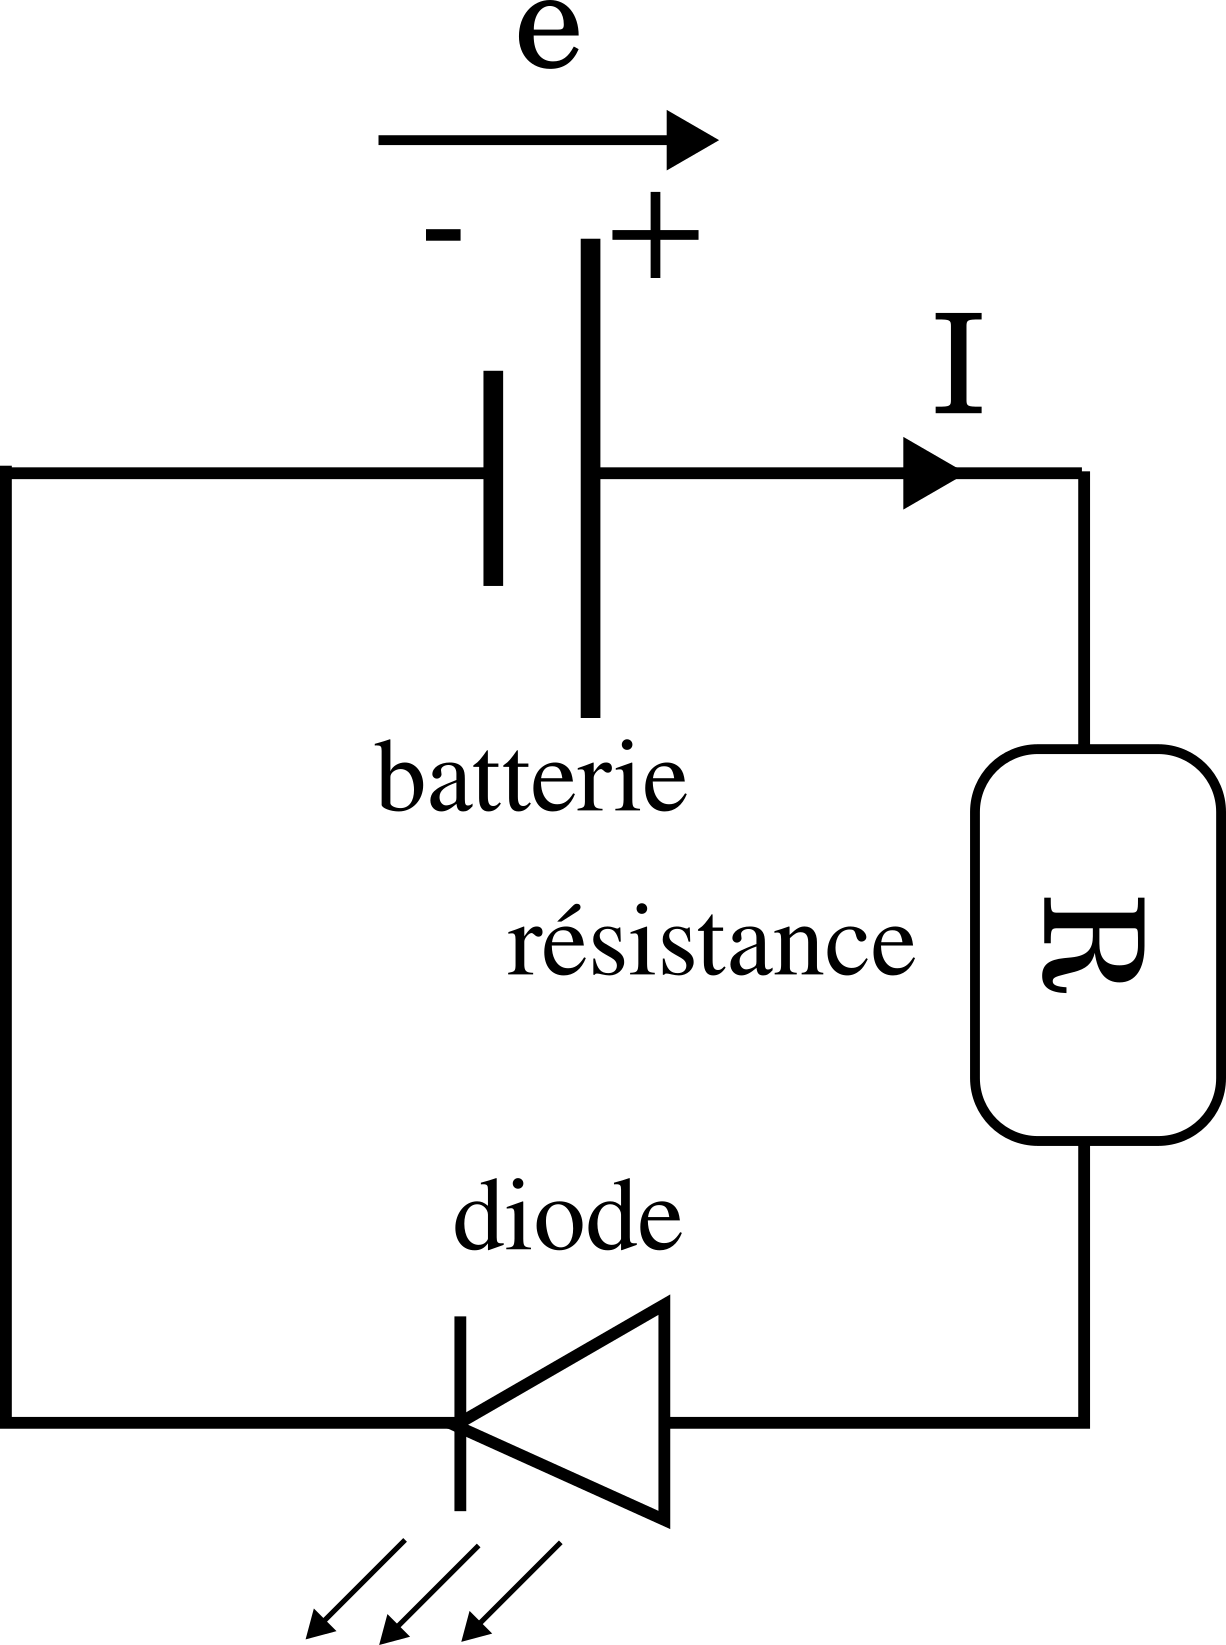
\includegraphics[height=3cm]{figures-Chp0/Fig03b}}\subfloat[\label{fig:03d}]{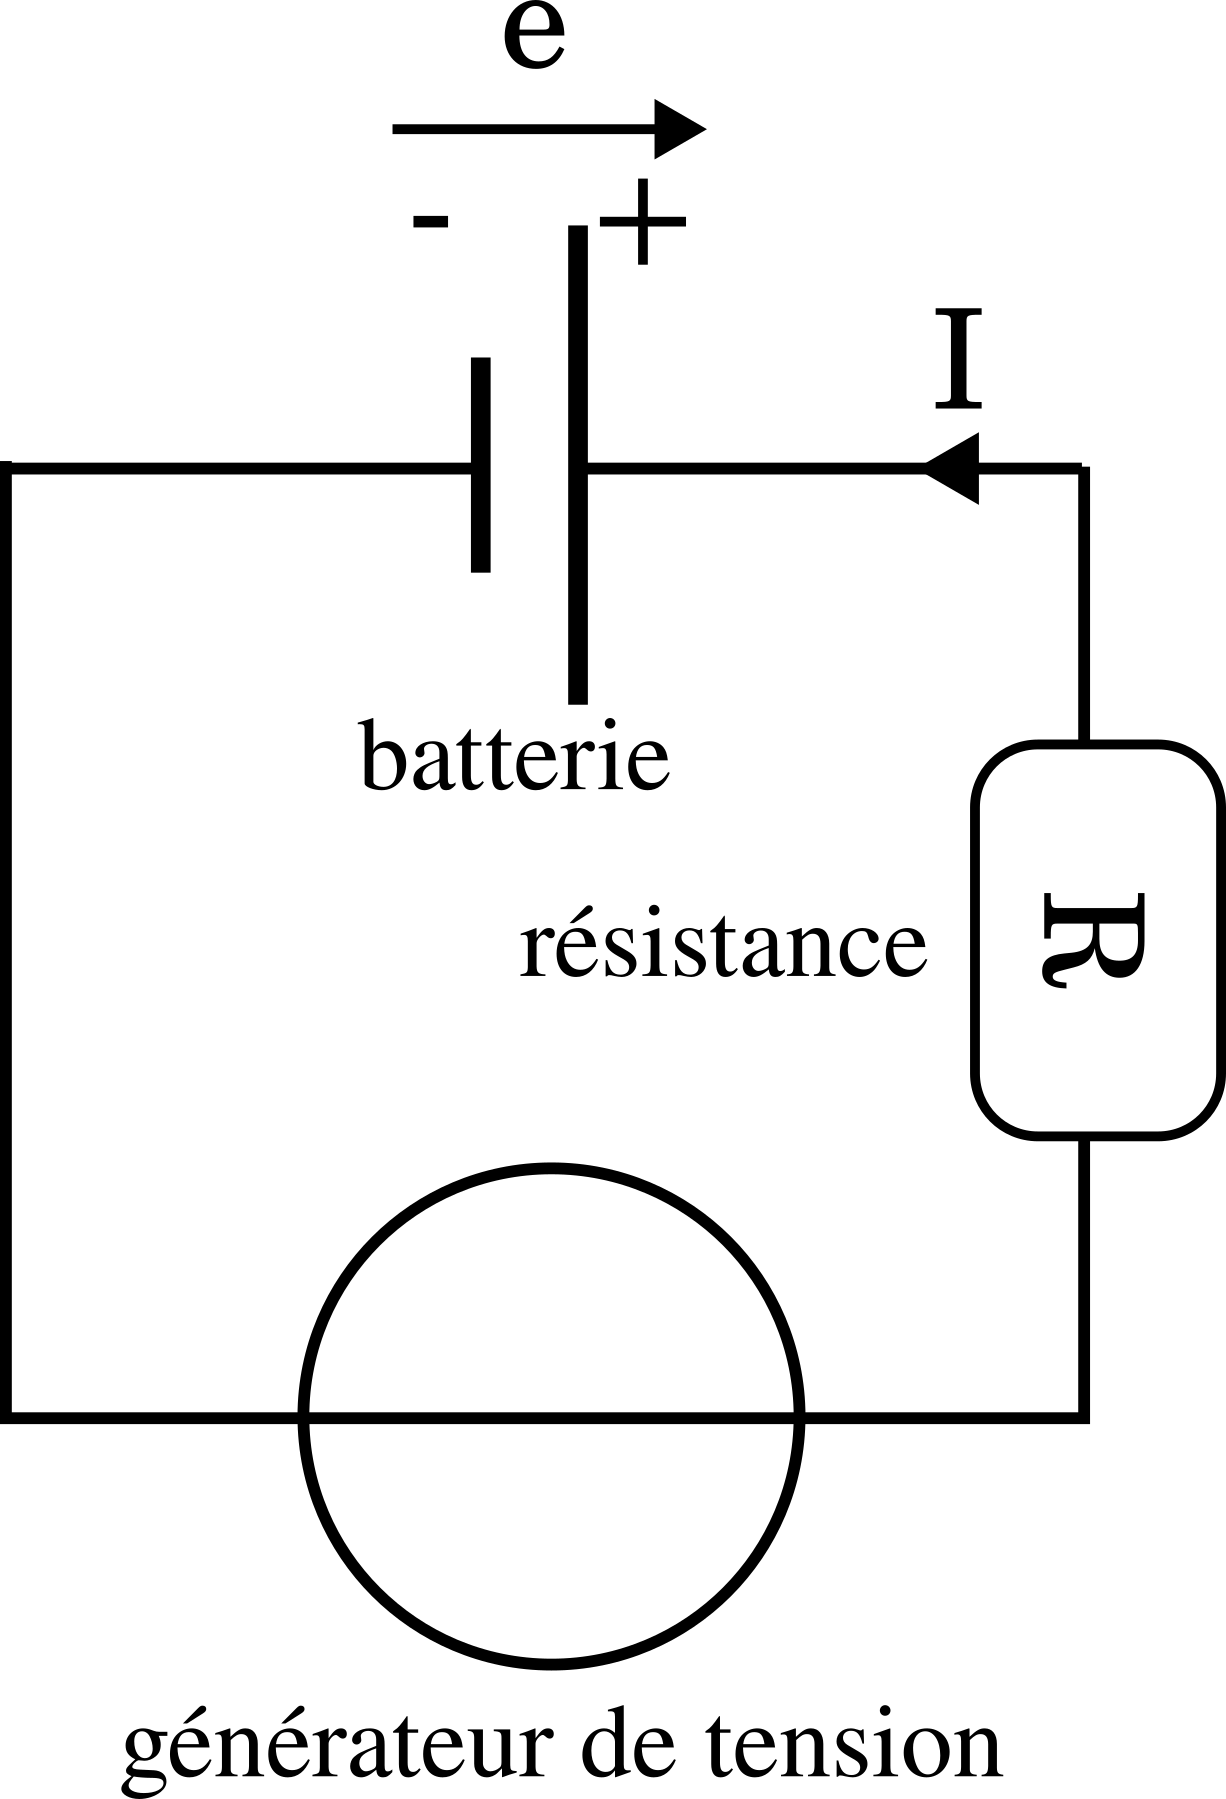
\includegraphics[height=3cm]{figures-Chp0/Fig03d}}
%\par\end{centering}
{\tiny{}\caption{{\small{} Fig. \ref{fig:03a}) Représentation schématique d'une pile AAA alimentant d'une résistance et une diode électroluminescente rouge ; Fig. \ref{fig:03b}) Circuit électrique équivalent ; \ref{fig:03c}) Représentation schématique d'une pile AAA et d'une résistance alimentée par un générateur en mode DC ; Fig. \ref{fig:03d}) Circuit électrique équivalent.}}
}{\tiny\par}
\end{figure}%WARNING : mettre U_B pour la tension de la batterie

\definition{

\blancbis{La pile électrique} est un dispositif électrochimique qui génère de l'électricité en convertissant de l'énergie chimique en énergie électrique grâce à une \blancbis{réaction d'oxydoréduction irréversible}.

~

\blancbis{L'accumulateur} est un dispositif électrochimique qui génère (resp. reçoit) de l'électricité en convertissant de l'énergie chimique (resp. électrique) en énergie électrique (resp. chimique) grâce à \blancbis{une réaction d'oxydoréduction réversible}. 
}

Si la pile AAA, illustré Fig. \ref{fig:03a}/\ref{fig:03b}, peut-être rechargée par le générateur, on peut dire qu'elle est constituée d'accumulateurs. Sinon, elle est constituée de piles.


Du point de vue électrique, l'accumulateur est :
\begin{itemize}
\item un \blancbis{générateur électrique} lorsqu'il se décharge ;
\item un \blancbis{récepteur électrique} lorsqu'il se charge.
\end{itemize}

La pile est quant à elle uniquement un \blancbis{générateur électrique}.


\subsection{Dispositifs constitués de plusieurs cellules électrochimiques}

\blancbis{La batterie} est le nom donné à tout dispositif électrique résultant de la mise en \blancbis{série} et/ou en \blancbis{parallèle}\mySideNote{\`{A} vous de deviner pourquoi une batterie a pour symbôle électrique : 
\begin{center}
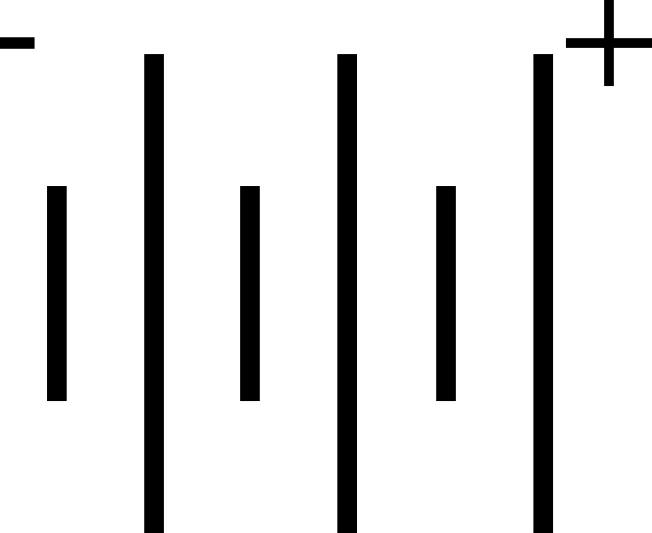
\includegraphics[width=2cm]{figures-Chp0/Fig05}
\end{center}} de plusieurs piles ou accumulateurs. On les classe alors en deux catégories : 
\begin{enumerate}
    \item primaire lorsque l'on a mis en série des piles ;
    \item secondaire lorsqu'on l'on a mis en série des accumulateurs.
\end{enumerate}

Ainsi, tout générateur primaire ne peut être utilisé \blancbis{qu'une seule fois}, et doit être jeté après utilisation. 

\section{Vocabulaire associé aux réactions électrochimiques}
Avant d'aborder les différentes parties d'une batterie, il est important de remettre en place quelques termes de vocabulaire propre aux réactions électrochimiques.

Afin de modéliser le flux d'électron, il est possible de décomposer l'équation de réaction en deux demi-équations rédox\mySideNote{\'{E}quation modélisant la transformation chimique au sein d'un couple rédox} modélisant chacune une \blancbis{oxydation} et une \blancbis{réduction}.

\definition{L'oxydation (resp. la réduction) correspond au processus chimique durant lequel une espèce \blancbis{libère} (resp. \blancbis{capte}) un (ou plusieurs) électron(s).}

Dans le cas d'une pile Daniell, pile impliquant les espèces rédox\mySideNote{On qualifiera de rédox, toute espèce chimique réactive réagissant par transfert d'électron(s). On peut qualifier ces espèces d'électroactives, par opposition aux espèces ne pouvant pas transférer d'électron(s) dites électroinactives.} suivantes : \ce{Cu^{2+}} et \ce{Zn}.

On peut écrire les demi-équations de réactions suivantes :

\begin{center}
\begin{minipage}{0.4\textwidth}
\begin{align*}
    \ce{Cu^{2+} (aq) + 2e^- &= Cu (s)} \\
    \ce{Zn(s) &= Zn^{2+} (aq) + 2e^- } \\
\end{align*}
\end{minipage}    
\end{center}

La première (resp. deuxième) demi-équation rédox correspond à la \blancbis{réduction} (resp. l'\blancbis{oxydation}). La combinaison linéaire de ces deux demi-équations constitue l'équation de réaction\mySideNote{Dans le cas des piles ou des accumulateurs, elle est parfois qualifiée de "fictive" au sens où cette réaction chimique n'a pas lieu dans un unique compartiment.} : 

\begin{align*}
\ce{Cu^{2+} (aq) + Zn(s) &= Cu (s) + Zn^{2+} (aq)}
\end{align*}

Cette réaction est dissymétrique, d'un côté une espèce gagne des électrons, de l'autre une espèce perd des électrons.

\definition{Le \blancbis{réducteur} est l'espèce chimique qui \blancbis{cède} des électrons, tandis que l'\blancbis{oxydant} en \blancbis{gagne}.} 

Dans l'équilibre chimique précédent, on peut identifier l'oxydant et le réducteur :

\begin{align*}
\underbrace{\ce{Cu^{2+}}}_{oxydant} (aq) + \underbrace{\ce{Zn(s)}}_{réducteur} &= \ce{Cu (s)} + \ce{Zn^{2+} (aq)}
\end{align*}

Pour identifier l'espèce qui cède/gagne des électrons, il faut écrire \blancbis{les demi-équations rédox} ou calculer \blancbis{la variation du nombre d'oxydation} des espèces\mySideNote{Le nombre d'oxydation, aussi appelé degré d'oxydation, est une grandeur qui caractérise le déficit d'électron d'un ion par rapport à l'élément chimique neutre.}. On peut donc identifier le couple oxydant/réducteur de deux manières différentes :

\begin{center}
\begin{minipage}[]{5cm}
\centering Demi-équations rédox

\begin{equation*}
\ce{Oxydant + ne^- = Reducteur}
\end{equation*}

\end{minipage}\hspace{0.5cm}\vline\hspace{0.5cm}\begin{minipage}[]{5cm}
\centering Variation du nombre d'oxydation

\begin{align*}
\Delta no (X) > 0 &\implies \text{oxydation} \\
\Delta no (X) < 0 &\implies \text{réduction} \\
\end{align*}

\end{minipage}
\end{center}

\example{
\textbf{Demi-équations rédox}
\begin{center}
\begin{align*}
\ce{Cu^{2+} (aq) + 2e^- &= Cu (s)} \\
\ce{Zn(s) &= Zn^{2+} (aq) + 2e^- }
\end{align*}
\end{center}
\textbf{Nombre d'oxydation}
\begin{align*}
\Delta no(\ce{Cu}) < 0 &\implies \text{réduction du cuivre} \\
&\implies \text{le cuivre est l'oxydant} \\
\Delta no(\ce{Zn}) > 0 &\implies \text{oxydation du zinc} \\
&\implies \text{le zinc est le réducteur}
\end{align*}}

\definition{Deux entités chimiques faisant partie d'une même équation rédox forment un couple rédox, noté le plus souvent par :
\begin{align*}
\text{Oxydant}/\text{Réducteur}
\end{align*}
}

Puisque le flux d'électron est \blancbis{orienté} dans un couple \ce{Ox}/\ce{Red}, il en résulte qu'à l'échelle macroscopique, les batteries forment des dispositifs \blancbis{orientés} électriquement.
\begin{comment}
\exercice{Indiquer les demi-équation rédox et si il s'agit de la modélisation d'une oxydation/réduction sachant que les couples rédox mis en jeux sont les suivants :
\begin{enumerate}
    \item \ce{Li^+ (aq)} / \ce{Li (s)} \& \ce{H2O (l)}/\ce{H2 (g)} ; 
    \item \ce{PbO2} (s) / \ce{Pb^{2+} (aq)} \& \ce{Pb^{2+}} (aq) / \ce{Pb (s)}%voir peut-être retirer SO42-
\end{enumerate}
Dans les réactions suivantes, identifier l'oxydant et le réducteur.

\ce{Li (s) + H2O (l) = Li^+ (aq) + HO^- (aq) + \frac{1}{2} H2 (g)}

\ce{PbO2 (s) + Pb (s) + 2 H2SO4 (aq) = 2PbSO4 (aq) + 2 H2O (l)}
}\end{comment}



\section{Description d'une batterie}
\subsection{Partie électroactive}
La description que nous allons faire traite de manière indifférente les batteries primaires et secondaires. En ces termes, piles et accumulateurs porteront le nom générique de cellule.

Toute cellule est un dispositif composé de $\ldots$

\paragraph*{$\ldots$ deux électrodes} dont l'une sert à capter les électrons et l'autre sert à céder des électrons. Une cellule est, par conséquent, un \textbf{dipôle électrique orienté}, c'est-à-dire composé d'un pôle $\oplus$ et d'un pôle $\ominus$.

La \blancbis{polarisation} électrique\mySideNote{Lorsque l'on parle de polarisation électrique, on sous-entend qu'il existe un pôle $\oplus$/$\ominus$ non confondu.} d'une cellule électrochimique ou batterie est invariante, peu importe le rôle joué au sein d'un circuit électrique.

\`{A} la Fig. \ref{fig:03b}, la batterie joue le rôle de générateur, c'est elle qui va imposer le sens du courant $I$ (donc le sens des électrons). \`{A} la Fig. \ref{fig:03d}, la batterie joue le rôle de récepteur, c'est donc le générateur de tension qui impose la polarisation. Dans les deux cas, les pôles de la batterie sont inchangés\mySideNote{Dans un générateur (resp. récepteur) électrique, le courant sort (resp. entre) par le pôle $\oplus$}. 

Le pôle, concept purement électrique, ne donne aucune information apparente sur la chimie au sein des demi-piles. On oriente chimiquement la batterie à l'aide des termes \blancbis{cathode}/\blancbis{anode}.

\definition{En décharge, le pôle $\oplus$ (resp. $\ominus$) d'une batterie est qualifié de \blancbis{cathode} (resp. \blancbis{anode}) lorsqu'il est le siège d'une réaction de \blancbis{réduction} (resp. d'\blancbis{oxydation}).}

Il existe une juste correspondance entre les termes électrique et les phénomènes chimiques ayant lieu, qui est résumé à la Tab. \ref{tab:Chp-0-conventions}.

\begin{center}
\begin{tabular}{|C{2.5cm}|C{3cm}|C{2cm}|C{2cm}|}
\hline
& & \multicolumn{2}{c|}{Polarisation électrique} \\
\hline
& & $\ominus$ & $\oplus$ \\
\hline
\multirow{2}{*}{Rôle électrique} & Générateur & anode & cathode \\
& Récepteur & cathode & anode \\
\hline
\end{tabular}
\captionof{table}{Relation entre électricité et chimie dans une cellule électrochimique ou une batterie.}
\label{tab:Chp-0-conventions}
\end{center}
%Rôle joué par la cellule dans le circuit

\attention{
Par abus de langage, les chimistes portant peu d'intérêt au rôle de la batterie au sein d'un circuit électrique utilise le terme anode (resp. cathode) en parlant du pôle $\ominus$ (resp. anode) en prenant comme référence la cellule ou batterie en décharge.\\

Il va de soi, qu'en toute rigueur, il faut nommer la demi-pile par ses pôles (puisque c'est l'invariant).
}


\subsection{Partie électroinactive}

Dans le cas d'une pile Daniell, pile utilisant les couples \ce{Cu^{2+}(aq)}/\ce{Cu(s)} et \ce{Zn^{2+}(aq)}/\ce{Zn(s)}, le dispositif peut se présenter de la manière suivante :

\begin{minipage}[c]{0.65\textwidth}
\centering
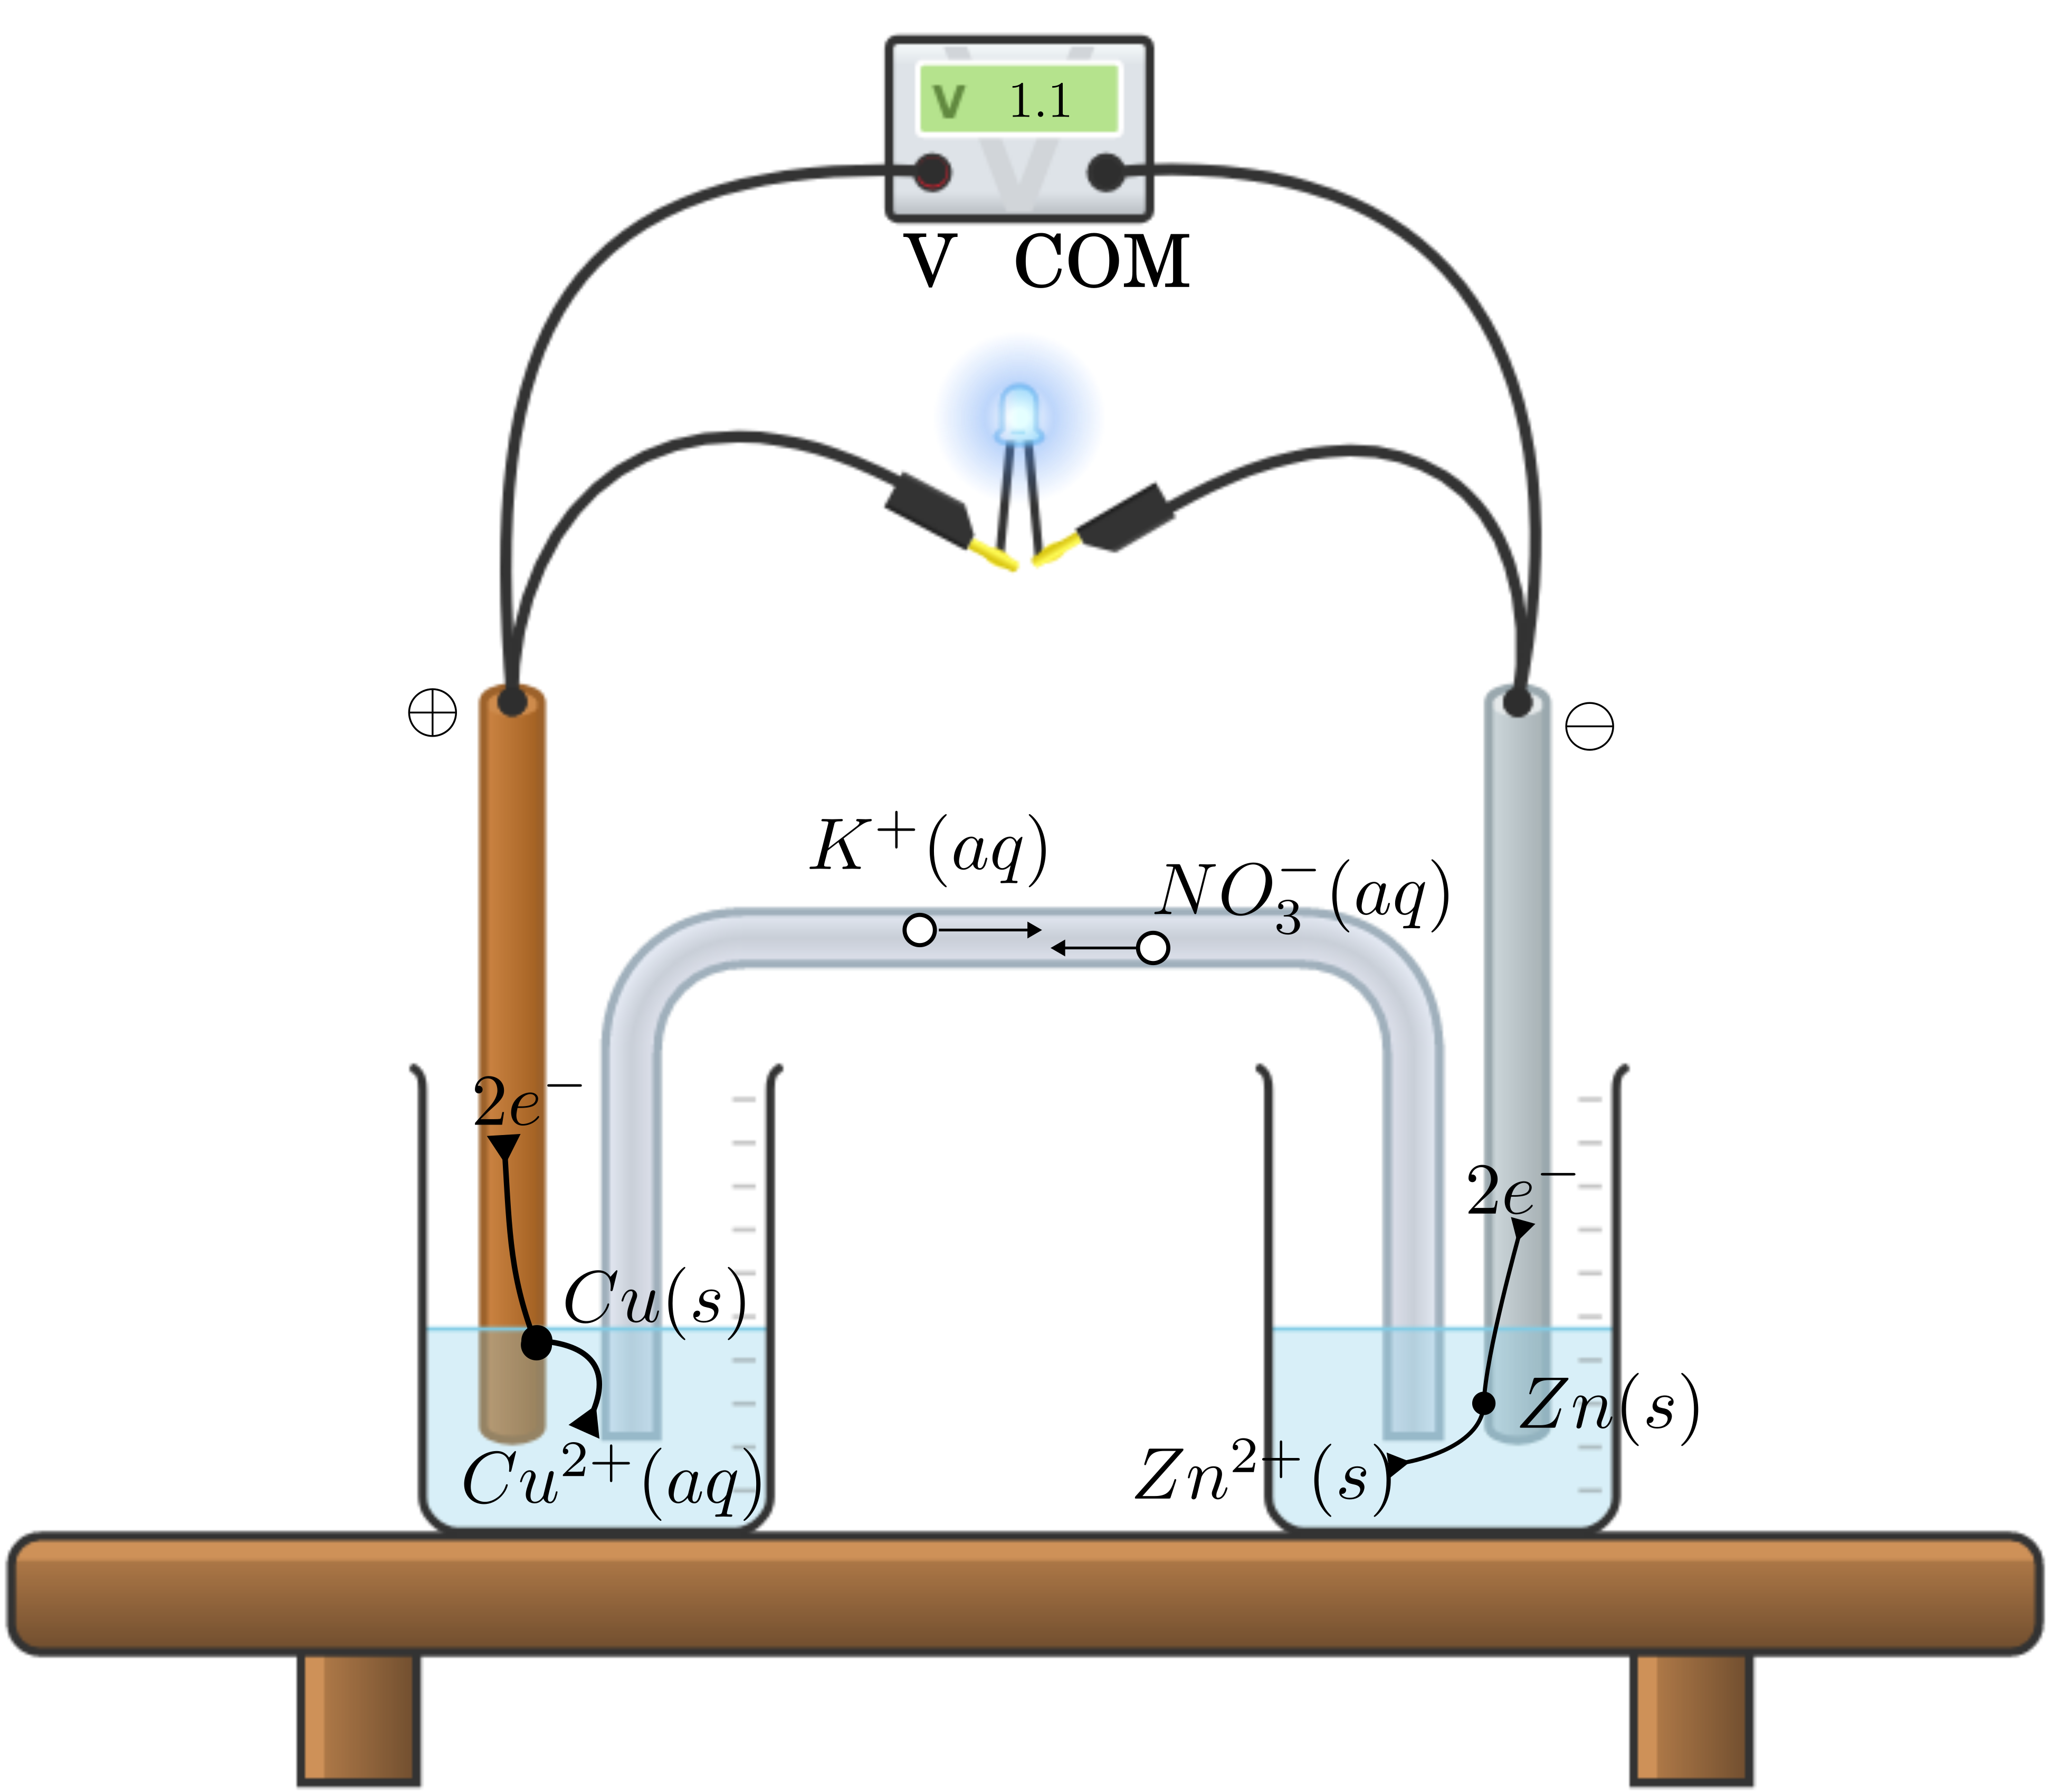
\includegraphics[width=8cm]{figures-Chp0/Fig04.png}
\end{minipage}\hfill   
\begin{minipage}[c]{0.35\textwidth}     
\captionof{figure}{Pile Daniell réalisée à l'aide :}
\begin{itemize}
    \item d'une solution de sulfate de cuivre accompagné d'une plaque de cuivre (cathode) ;
    \item d'une solution de sulfate de zinc accompagné d'une plaque de zinc (anode).
\end{itemize}
\label{fig:04}
\end{minipage}

Le dispositif peut se résumer de la manière suivante : 
\begin{equation*}
\ominus \quad \ce{Zn(s)} | \ce{Zn^{2+} (aq)}; \ce{SO_4^{2-} (aq)} | K^+ (aq), NO_3^- (aq) | \ce{Cu^{2+} (aq)}; \ce{SO_4^{2-} (aq)} | \ce{Cu(s)} \quad \oplus
\end{equation*}
en indiquant par $|$ les interfaces entre les différentes phases.


Une des premières choses à remarquer est que les fils électriques permettent de fermer le circuit électrique, tandis que le pont salin contenant une solution de \ce{KNO3} concentrée permet de fermer la partie chimique. Si le circuit n'est pas fermé dans la partie chimique ou la partie électrique, un ampèremètre branché aux bornes de la cellule indiquera un courant nul\mySideNote{Ceci n'est qu'un constat expérimental qui servira de généralisation. En réalité, il est tout à fait possible de démontrer cette observation grâce aux lois de l'électrostatique.}.

%\mySideNote{La migration est le terme associé à la mise en mouvement d'une particule chargée sous l'action d'un champ électrique. Ce terme est à mettre en perspective avec la diffusion et la convection. Ces phénomènes, dit de transport, seront traité en S4.06.}

\definition{
\blancbis{Solvant} ~  Il s'agit de l'espèce permettant de \blancbis{solvater} les espèces rédox et électrolytiques.

~

\blancbis{Electrolyte} ~  Afin de fermer le circuit électrique et permettre la circulation des électrons, le courant doit pouvoir circuler dans la cellule. Contrairement aux fils et électrodes, où le courant est assuré par les électrons, dans la solution et le séparateur, le courant est assuré par la \blancbis{migration} des ions.

Celui-ci est choisi en fonction de deux contraintes : 
\begin{enumerate}
    \item diminuer la résistivité des compartiments anodiques et cathodiques ;
    \item garantir le processus de migration au sein de la solution.
\end{enumerate}

~

\blancbis{Séparateur} ~  En général, les cellules sont composées d'un séparateur qui permet de séparer \blancbis{physiquement} et \blancbis{spécifiquement} les espèces électroactives du compartiment anodique et cathodique. Le séparateur est soit une membrane, soit un pont salin. Ce séparateur obéit à deux contraintes : empêcher toute réaction parasite entre espèces électroactives, tout en assurant une bonne conductivité ionique d'espèces chimiques chargées, mais inertes chimiquement.
}

L'ensemble chimique électrolyte, solvant et séparateur, qualifié d'\blancbis{électroinactif}, joue un rôle clef dans le fonctionnement d'une batterie/pile mais ne sera quasiment jamais abordé dans ce module où on s'intéressera avant tout au design de la partie électroactive.\mySideNote{L'électrolyte support est parfois une (ou des espèces) électroactive(s), comme dans le cas de la pile Daniell.} En général, on se limitera à écrire les espèces électroactives : 

\begin{equation*}
\ominus \quad \ce{Zn(s)} | \ce{Zn^{2+} (aq)} || \ce{Cu^{2+} (aq)} | \ce{Cu(s)} \quad \oplus
\end{equation*}

Sauf si on a besoin des autres espèces pour comprendre le problème physique.

\subsection{Batterie, tension électrique et force électromotrice}

\begin{figure}[H]
\begin{center}
\begin{tabular}{cc}
\subfloat[\label{fig:Chp0-16a}]{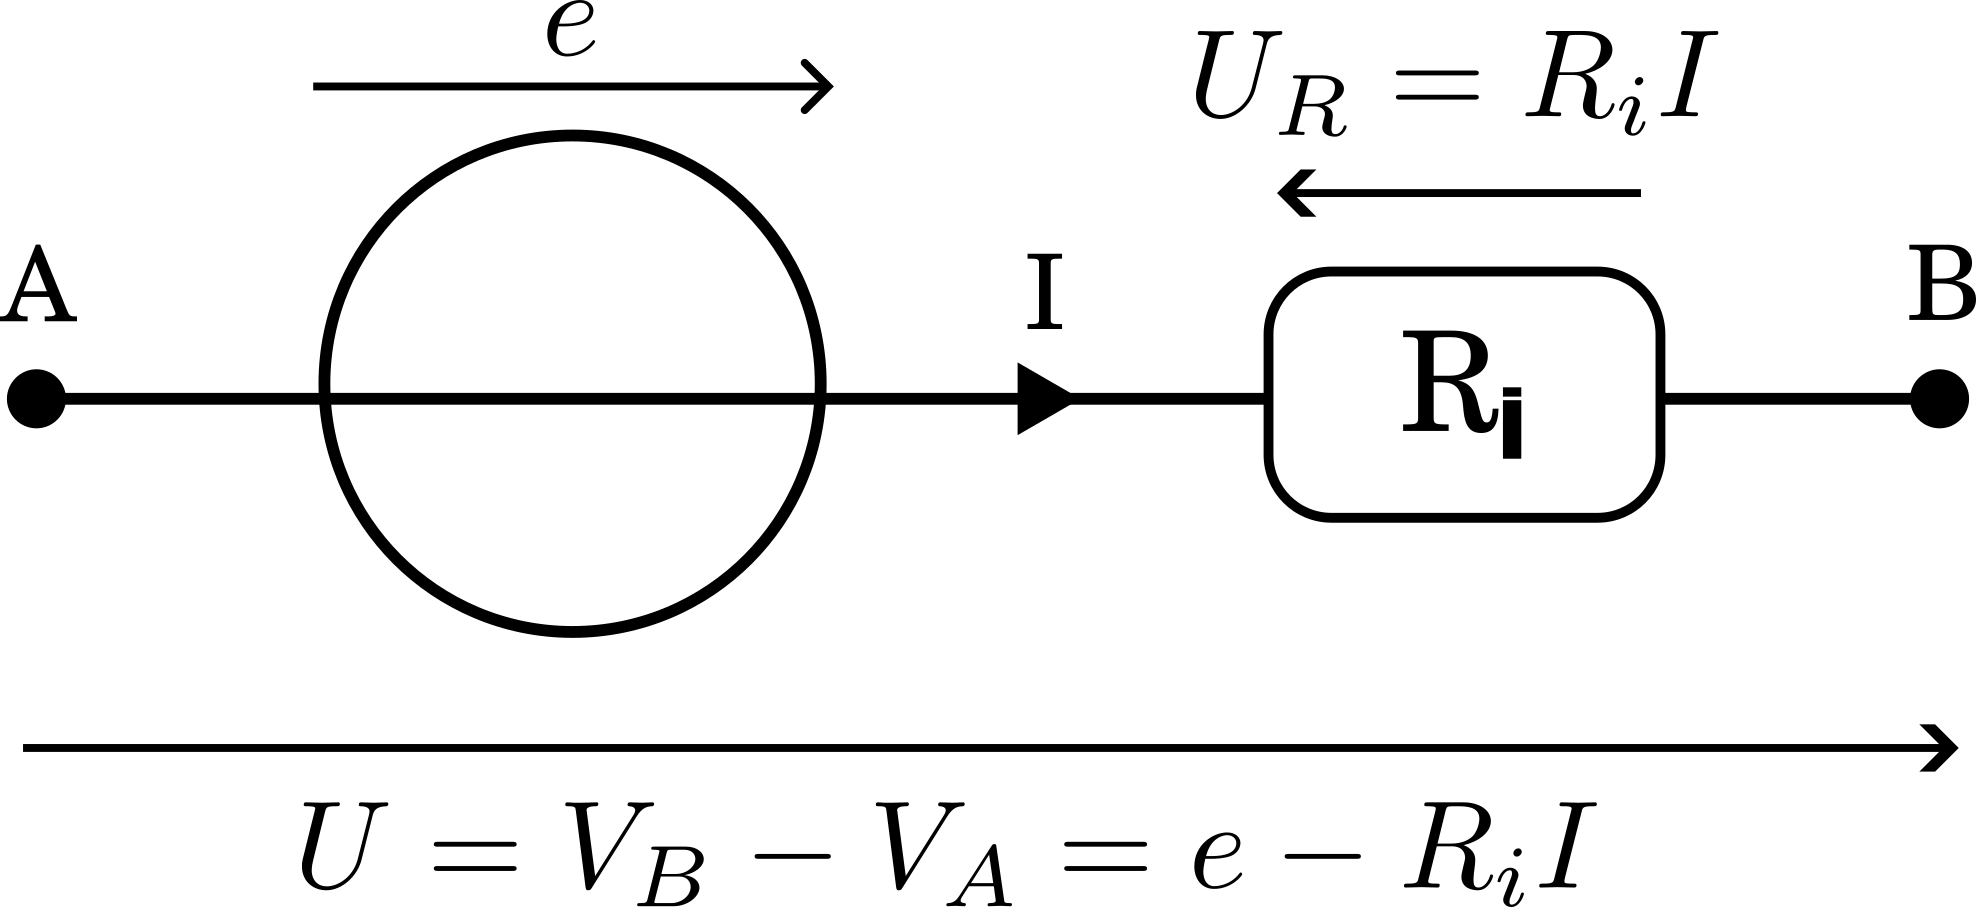
\includegraphics[width=0.48\textwidth]{figures-Chp0/Fig16a}} & \subfloat[\label{fig:Chp0-16b}]{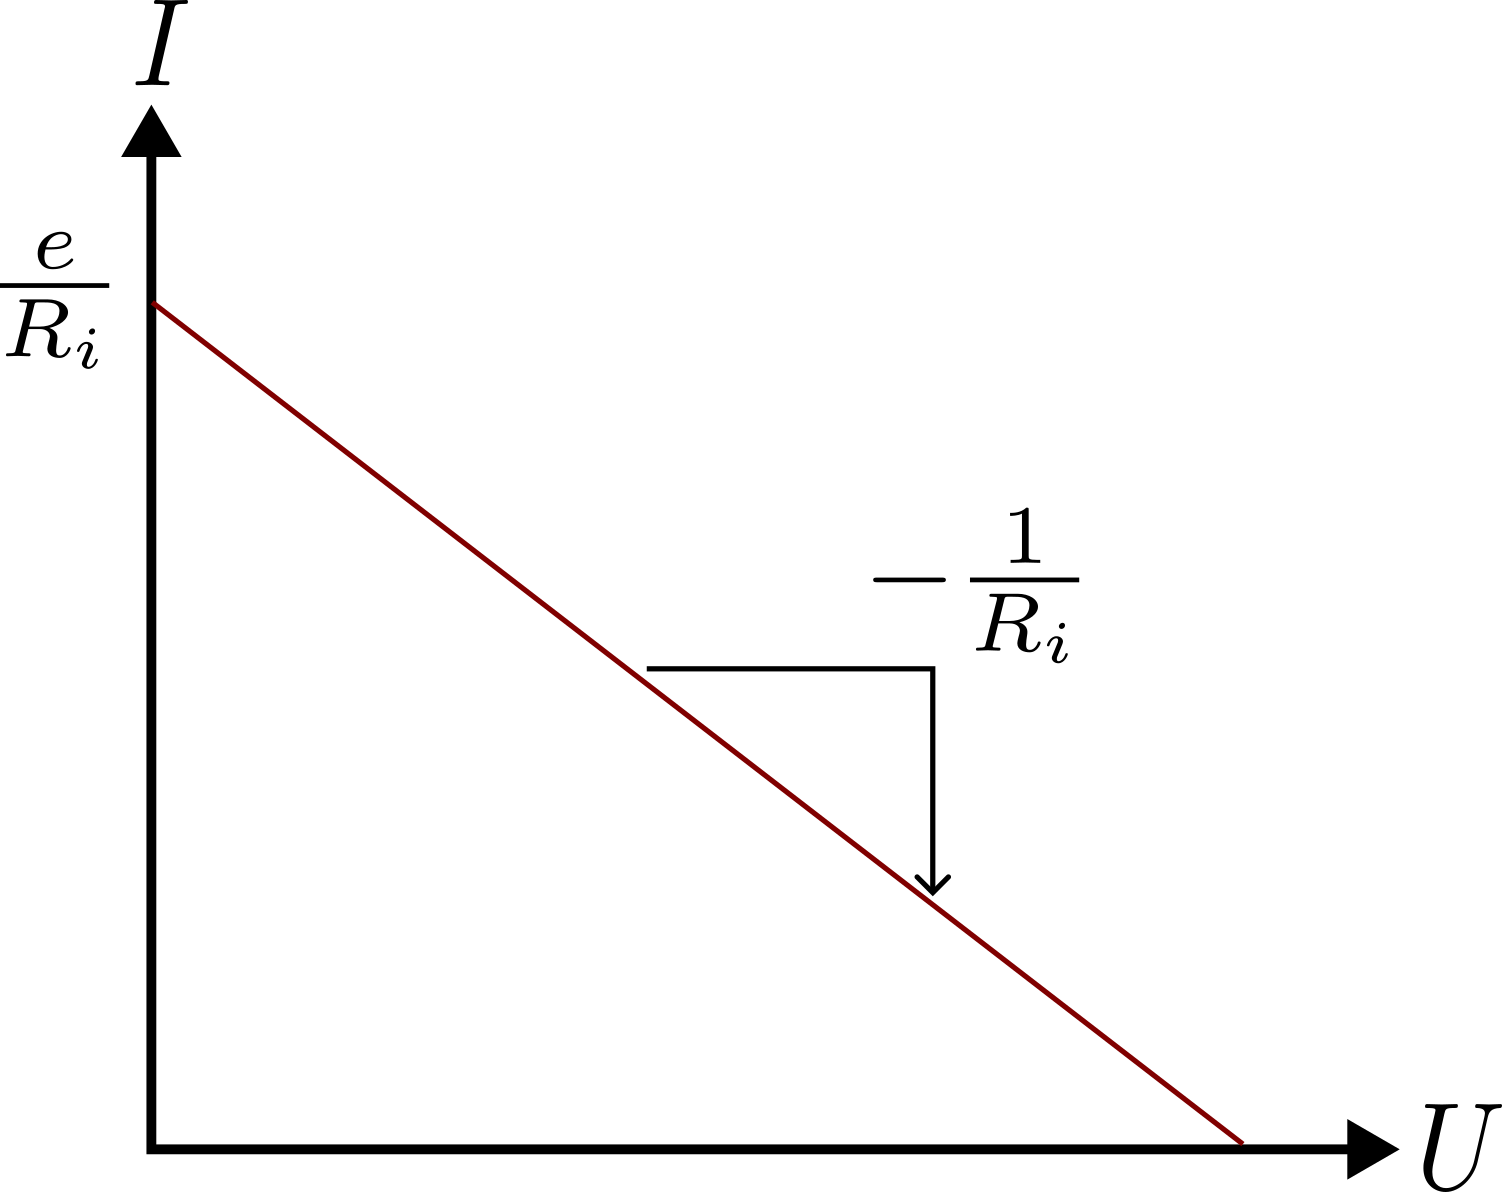
\includegraphics[width=0.30\textwidth]{figures-Chp0/Fig16b}}
\end{tabular}
\end{center}
\caption{\ref{fig:Chp0-16a} Modèle de Thévenin permettant la description de la caractéristique d'une cellule électrochimique ; \ref{fig:Chp0-16b} Allure de la caractéristique d'une cellule électrochimique}
\end{figure}

Lorsque l'on mesure la tension aux bornes d'une cellule électrochimique, notée $U$, on mesure une différence de potentiel électrique entre les deux pôles de la pile. Cette tension électrique dépend de deux paramètres électriques comme représenté à la Fig. \ref{fig:04} :\mySideNote{Ces grandeurs ont été vu en Physique en S1.} 
\begin{itemize}
\item la \blancbis{tension à courant nul}, souvent appelée tension de circuit ouvert\mySideNote{On la rencontrera en TP sous le terme OCV pour \textbf{Open-circuit voltage}.} ;
\item la \blancbis{résistance interne}, notée $R_i$, de la cellule.%inclu résistance de polarisation
\end{itemize}

L'origine chimique de ce comportement pourra être expliqué à la suite d'un cours intensif de thermodynamique et de cinétique électrochimique et sera admis comme tel pour le moment.

Dans les études que nous allons faire sur les batteries, nous chercherons avant tout à établir un lien structure/propriété entre la \emph{tension à courant nul} et la structure chimique aux électrodes. En effet, la tension à courant nul est associée à une grandeur thermodynamique, appelée force électromotrice et notée $e$ qui quantifie la force électrique permettant de séparer les charges au sein de la batterie



\example{
Le voltmètre dispose d'une très grande résistance (idéal = résistance infinie), on va donc bien mesurer la tension à courant nul. De plus, si les électrodes sont des phases homogènes et isotropes macroscopiquement, le potentiel électrostatique est constant. On va pouvoir décomposer le potentiel électrique en fonction des différents points dans la batterie schématisée à la Fig. 

\begin{center}
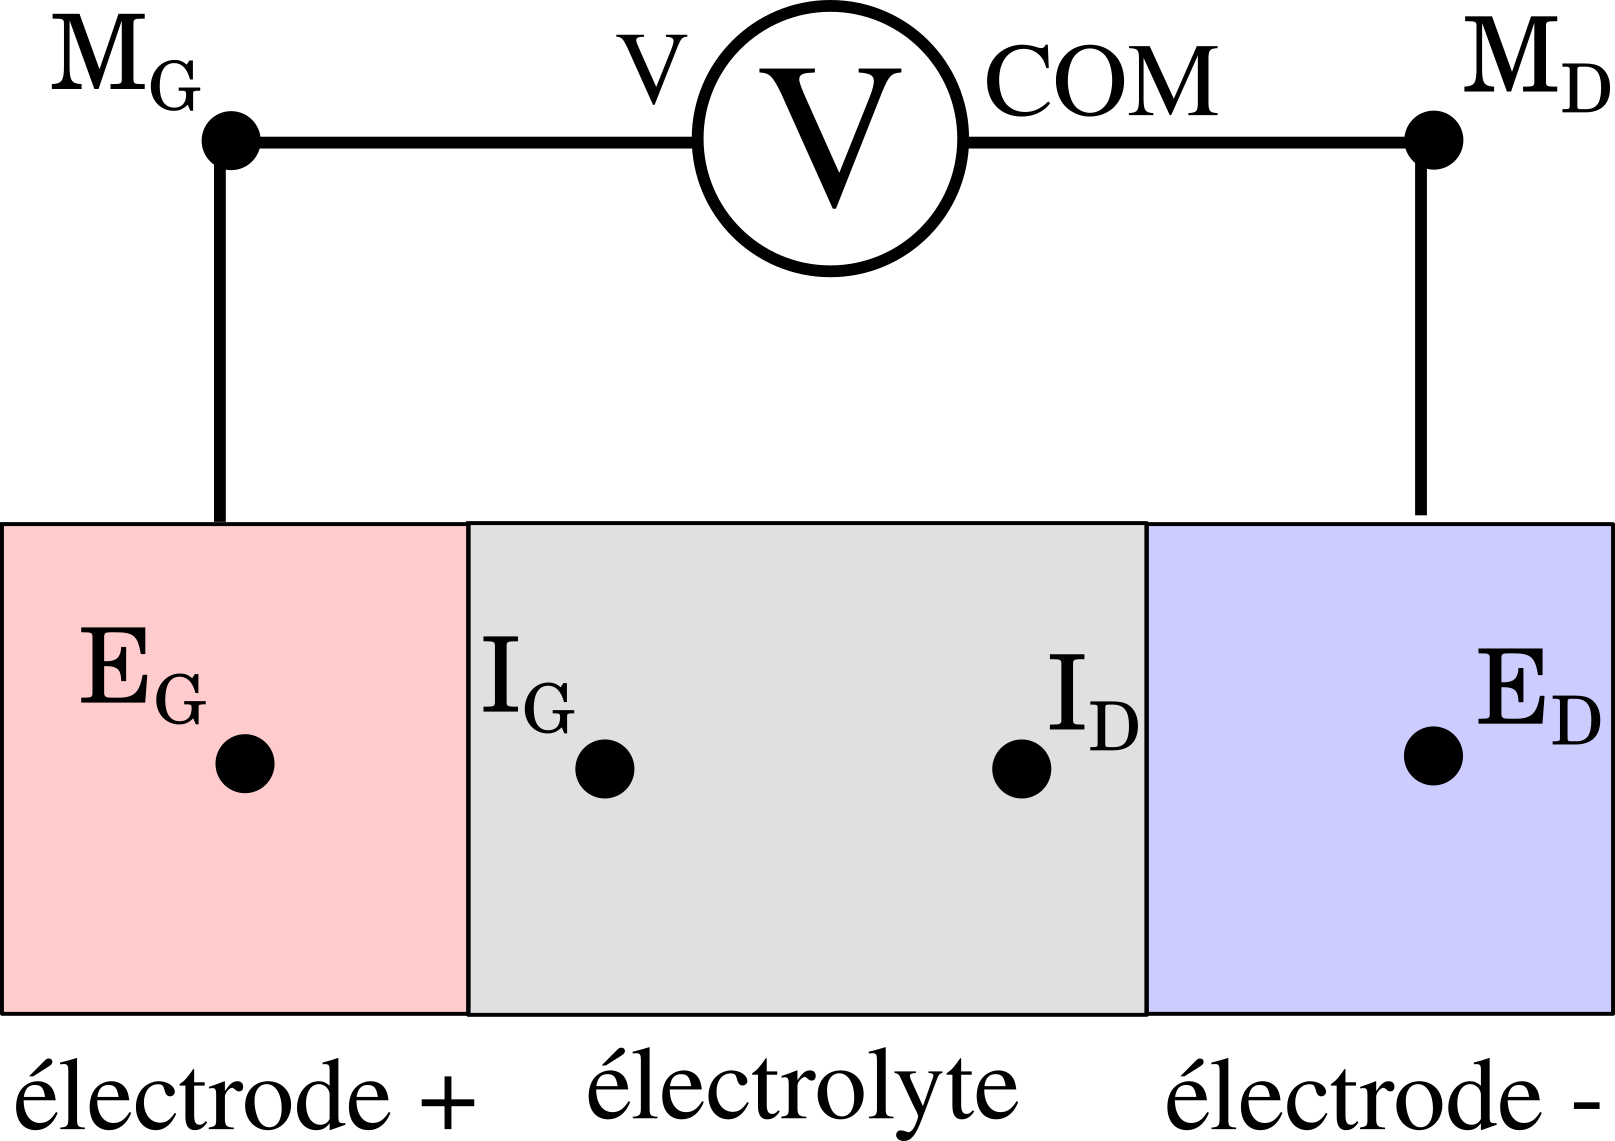
\includegraphics[width=5cm]{figures-Chp0/Fig06}
\captionof{figure}{Représentation des phases mises en jeux au sein d'une batterie (l'électrolyte suppose l'existence éventuelle d'une phase électrolytique en contact avec l'interface, ainsi que d'un éventuel pont salin).}
\end{center}

\begin{align*}
U( I=0 ~ \si{\ampere} ) &= \Phi (M_G) - \Phi (M_D) \\
&= \underbrace{\left ( \Phi (M_G) - \Phi (E_G) \right )}_{K} + \underbrace{\left ( \Phi (E_G) - \Phi (I_G) \right )}_{E_\oplus} \\
& + \underbrace{\left ( \Phi (I_G) - \Phi (I_D) \right )}_{E_j} - \underbrace{\left ( \Phi (E_D) - \Phi (I_D) \right )}_{E_\ominus} \\
& - \underbrace{\left ( \Phi (M_D) - \Phi (E_D) \right )}_{K}
\end{align*}

On remarque cinq termes :
\begin{enumerate}
\item deux potentiels d'interface entre les fils de cuivre et les électrodes, noté $K$. En général, il s'agit un terme constant qui disparaît lorsque l'on étudie des différences de potentiel (ce que l'on fait toujours) ;
\item le potentiel d'électrode au pôle $\oplus$, noté $E_\oplus$ ; 
\item le potentiel de jonction, noté $E_j$ ; 
\item le potentiel d'électrode au pôle $\ominus$, noté $E_\ominus$.
\end{enumerate}

En général, expérimentalement, le potentiel de jonction est négligeable devant la différence des potentiels d'électrode, ce qui nous laisse : 

\begin{align}
U ( I=0 ~ \si{\ampere} ) &= E_\oplus - E_\ominus + E_j  \\
& \approx E_\oplus - E_\ominus
\end{align}}

La tension à courant nul est donc pas définition lié à une différence de potentiel électrique entre l'électrode $\oplus$ et l'électrode $\ominus$. Cette différence de potentiel sous entend l'existence éventuelle d'un champ électrique au sein de la pile, que l'on appelle la force électromotrice de la réaction.

\attention{Dans le restant du cours, nous ferons l'amalgame couramment fait par les chimistes : assimiler la force électromotrice, siglé f.e.m et notée $e$ à la tension à vide $U(I=0 ~ \si{\ampere})$}

\section{Type de réactions}

On va chercher à classer les réactions des cellules électrochimiques utilisant du lithium en deux grandes catégories : 
\begin{enumerate}
\item les cellules qui conduisent à l'apparition et la disparition d'une phase contenant des ions lithiums ;
\item les cellules dans lesquelles les matériaux sont des "éponges" d'ions lithium et sont capables de les accueillir sans qu'il y ait apparition/disparition d'une phase.
\end{enumerate}

Par exemple, un des première batterie brevetée en 1977 par S. Whittimgham utilisait un pôle $\ominus$ en lithium métallique et un pôle $\oplus$ en \ce{TiS2} : 
\begin{center}
\begin{minipage}{0.58\textwidth}
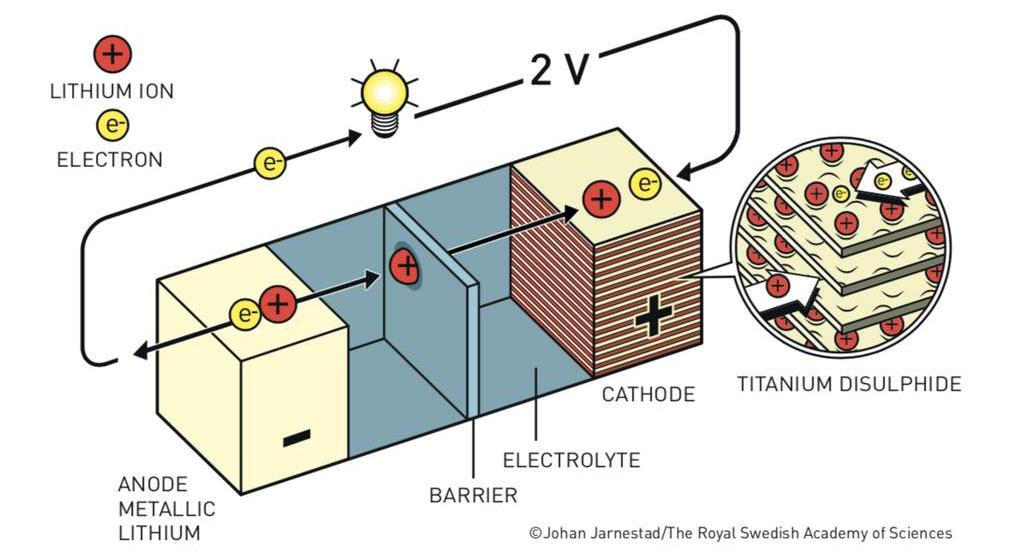
\includegraphics[width=\textwidth]{figures-Chp0/Fig18}
\end{minipage}\hfill\begin{minipage}{0.38\textwidth}
\captionof{figure}{Cellule électrochimique de S. Whittimgham.}
\end{minipage}\end{center}
On voit que \ce{TiS2} est un matériau fonctionnant comme une "éponge" à ions lithium.

\subsection{Réactions de recomposition}

Dans de nombreuses réactions électrochimiques, on observe l'apparition ou la disparition de phases. Par conséquent, cela traduit d'importantes modifications des matériaux d'électrodes, appelé \blancbis{recomposition}.

\subsubsection{dites de formation}

\definition{Une réaction de \blancbis{formation} est une réaction de \blancbis{recomposition} où deux phases réagissent ensemble pour conduire à la formation d'une \blancbis{troisième}. Elles sont modélisées par une équation de réaction de la forme : 
\begin{center}
A + B = AB
\end{center}
La phase AB est formée à partir des composants atomiques des phases A et B.}
%2 Li + Sb = Li2Sb


\subsubsection{dites de déplacement}

\definition{Une réaction de déplacement est une réaction de \blancbis{recomposition} dans laquelle une phase(s) (ou plusieurs) disparaî(ssen)t au profit d'une (de plusieurs) nouvelle(s) phase(s). Elles sont modélisées par une équation de réaction de la forme : 
\begin{center}
A + BX = AX + B
\end{center}
}%2 Li + Cu2O = Li2O + 2Cu

%%EXERCICE

\subsection{Réactions d'insertion}

Il existe une autre catégorie de réaction dans les systèmes électrochimiques où une espèce chimique rédox, accueillie au sein d'un matériau hôte stable migre, lors de la décharge, vers les sites interstitiels inoccupés d'un autre matériau stable.

%Image des deux cas de figure

En général, l'incorporation de l'espèce accueillie à lieu de manière topotactique\mySideNote{\'{E}spèces accueillies s'établissent dans des sites spécifiques de la structure cristalline.} et non pas de manière atactique\mySideNote{\'{E}spèces accueillies s'établissent dans des sites aléatoires de la structure cristalline.}.

\definition{Une réaction d'\blancbis{insertion} est une réaction où une \blancbis{solution solide disparaît} au profit de la \blancbis{formation} d'une nouvelle solution solide.

Elles sont modélisées par une équation de réaction de la forme : 
\begin{align*}
\ce{x A + BX = A_x BX}
\end{align*}
où \ce{A} désigne l'espèce accueillie et \ce{BX} désigne l'espèce hôte.

}
%WARNING Lix + TiS2 = Lix TiS2
Notons dès à présent que dans le cas des matériaux lamellaires\mySideNote{Voir Chp. 3}, les \blancbis{réactions d'insertion} sont parfois appelées \blancbis{réactions d'intercalation}.

\attention{Il est parfois possible qu'une réaction de déplacement se produise par remplacement d'une espèce interstitielle par une autre à l'intérieur d'un matériau hôte. Dans ce cas, une seule phase supplémentaire est formée et on parle d'\blancbis{extrusion} pour décrire ce processus.}
%HCl + LiMO2 = HMO2 + LiCl


\section{Caractériser un accumulateur ou une batterie}

\subsection{Charge, \'{E}nergie \& Puissance}
\subsubsection{Définition}
Les cellules électrochimiques sont des dispositifs électriques. Par conséquent, trois grandeurs électriques usuelles permettent de les caractériser : la charge (notée \textbf{q}), la tension (notée \textbf{U}) et le courant (notée \textbf{I}). Le courant dérive de la charge\mySideNote{Il faut savoir que :
\begin{align*}
I = \frac{dq}{dt}
\end{align*}
}.

Deux grandeurs dérivées des trois grandeurs fondamentales de l'électricité peuvent nous intéresser :

\begin{enumerate}
    \item la puissance électrique instantanée, notée $P$
    \begin{equation}
        P(t) = U(t) I(t)
        \label{eq:puissance}
    \end{equation}
    \item le travail électrique, noté $W'$
    \begin{equation}
        W' = \int_0^t P(t') dt' = \int_0^t U(t') I(t') dt'
        \label{eq:travail}
    \end{equation}
\end{enumerate}

Lorsque le dispositif électrique est en convention récepteur (resp. générateur), la relation Eq. \ref{eq:puissance} nous donne la puissance \blancbis{reçue} (resp. \blancbis{émie}) par le dispositif. De même pour la relation sur le travail Eq. \ref{eq:travail}.

\subsubsection{État de charge}
Afin de caractériser l'état d'une pile ou batterie, on peut utiliser diverses grandeurs dérivées de la capacité permettant de définir son état à un instant $t$.

\definition{
\blancbis{\'{E}tat de charge (SoC, State-of-Charge)} indique la quantité d'énergie emmagasinée par la cellule ou batterie. On la définit comme : 
\begin{equation*}
    SoC [\si{\percent}]= \frac{\text{charge emmagasinée par la batterie}}{\text{charge maximale que peut emmagasiner la batterie}} * 100
    \label{eq:SoC}
\end{equation*}}

Si $SoC =$ \SI{0}{\percent} (resp. \SI{100}{\percent}), la batterie est déchargée (resp. chargée)

\definition{
\blancbis{\'{E}tat de décharge (DoD, Depth-of-Discharged)} indique la quantité d'énergie non emmagasinée par la cellule ou batterie. On la définit comme : 
\begin{equation*}
    DoD [\si{\percent}]= \frac{\text{charge non emmagasinée par la batterie}}{\text{charge maximale que peut emmagasiner la batterie}} * 100
    \label{eq:DoD}
\end{equation*}}

Par définition, $DoD [\si{\percent}] = 100 - SoC [\si{\percent}]$. Si $DoD =$ \SI{0}{\percent} (resp. \SI{100}{\percent}), la batterie est chargée (resp. déchargée)

\subsection{Capacité spécifique (CS)}
\subsubsection{Définition}
La \blancbis{capacité d'une batterie} est définie comme la quantité maximale de charges qui peut être stockée dans la cellule ou batterie. Cette grandeur est \blancbis{extensive}, c'est-à-dire qu'elle dépend de la quantité de matériau présent.\mySideNote{Par opposition, la tension est intensive, elle ne dépend pas de la quantité de matériau présent.}

En général, les chimistes lui préfèrent la \blancbis{capacité spécifique}.

\definition{
La capacité spécifique, notée $CS$, est définie comme : 
\begin{itemize}
\item le rapport de la capacité sur la masse du dispositif, d'où l'appelation de capacité spécifique \blancbis{massique} : 
\begin{align*}
CS_m = \frac{\text{Charge maximale stockable}}{\text{Masse du dispositif}}
\end{align*}
\item le rapport de la capacité sur le volume du dispositif, d'où l'appelation de capacité spécifique \blancbis{volumique} :
\begin{align*}
CS_v = \frac{\text{Charge maximale stockable}}{\text{Volume du dispositif}}
\end{align*}
\end{itemize}

La capacité spécifique s'exprimera en \si{\coulomb\per\kilo\gram} ou \si{\coulomb\per\meter\cubed}
}

L'unité commerciale utilisée est le \si{\ampere\hour\per\kilo\gram}.

%WARNING def
\attention{La capacité \blancbis{spécifique} sera liée à la nature du matériau d'électrode.}

\subsubsection{\'{E}tat de santé (SoH, State-of-Health)} 

\definition{
L'état de santé (SoH, State-of-Health) indique la charge maximale réelle par rapport à la charge maximale théorique que peut contenir la cellule ou la batterie.
\begin{equation*}
    SoH [\si{\percent}]= \frac{\text{capacité maximale réelle}}{\text{capacité maximale théorique}} \times 100
    \label{eq:SoH}
\end{equation*}}

L'état de santé permet de caractériser l'état de vieillissement de votre pile. Si la pile est neuve (resp. usagée), alors $SoH =$ \SI{100}{\percent} (resp. $SoH \to$ \SI{0}{\percent}).

\subsection{Qualité de l'énergie stockée}

La puissance électrique, ainsi que l'énergie, sont liées à la tension à circuit ouvert et par extension à la f.e.m.\mySideNote{La force électromotrice pour ceux qui n'aurait pas suivi =P.}. Nous allons voir au chapitre suivant que la f.e.m. est directement liée à la thermodynamique de la réaction chimique "fictive" ayant lieu entre les espèces chimiques des deux compartiments. Elle est la force motrice permettant la circulation des électrons et le transport des ions à travers l'électrolyte.

En général, du point de vu électrique, la \blancbis{qualité de l'énergie électrique} est supérieure lorsque la tension électrique est élevée. Ceci est simple à comprendre, si vous alimentez une résistance $R$ avec votre pile de f.e.m $e$, la puissance reçue par la résistance est : 
\begin{equation}
P = U_R \cdot I = \frac{e^2}{R}
\end{equation} 

ainsi, du fait du terme en $e^2$; la puissance électrique reçu par un tel dispositif est très sensible à la tension. On peut arbitrairement donner quelques plages de tension, associées aux applications courantes, permettant de définir la qualité de la tension électrique : 
\begin{center}

\begin{tabular}{cc}
$3.5 - 5.5$ \si{\volt} & Grande qualité \\
$1.5 - 3.5$ \si{\volt} & Qualité moyenne \\
$0.0 - 1.5$ \si{\volt} & Qualité faible
\end{tabular}
\end{center}

Cependant, il peut exister des applications allant au délà de ces plages (\emph{par ex.} les voitures électriques nécessitent des tensions autour de \SI{200}{\volt})\mySideNote{Un chimiste ne cherchera pas forcément à optimiser la tension de sortie d'une cellule. En effet, pour certaines applications, comme les semi-conducteurs pour l'électronique, on cherchera en général à avoir de petites tensions (< \SI{1}{\volt}).}.

\subsection{\'{E}nergie théorique maximale (ETM)}
L'énergie théorique maximale est une grandeur permettant de prendre à compte la force électromotrice de la cellule ou batterie et la capacité spécifique et représente l'énergie électrique maximale pouvant être extraite, en théorie, d'une batterie.

\definition{
L'énergie théorique maximale, notée ETM, se définit comme le travail électrique : 
\begin{equation}
ETM = \text{force électromotrice} \times \text{capacité spécifique}
\end{equation}

Elle est en général exprimée en \si{\joule\per\kilo\gram}.}

L'unité commerciale utilisée est le \si{\watt\hour\per\kilo\gram}.

\subsection{Cyclabilité}
Lorsque l'on cherche à réaliser des dispositifs rechargeables, il est fondamental d'étudier \blancbis{la cyclabilité} des dispositifs, c'est-à-dire le nombre de cycle de charge/décharge qu'est capable de faire une batterie avant de perdre complètement sa capacité de charge.

Un dispositif peut être considéré comme toujours fonctionnel si ses caractéristiques électriques : capacité, force électromotrice, énergie stockée$\ldots$ ne sont pas dégradés malgré le cyclage.

On remarque à la Fig. \ref{fig:Chp-0-07}, que pour une perte de la capacité électrique de \SI{0.5}{\percent} à chaque cycle, valeur qui peut sembler anodine, une batterie perd \SI{40}{\percent} de ses capacités en 100 cycles\mySideNote{Tout le travail du chimiste, donc le votre, va être de parvenir à synthétiser des matériaux qui prémunissent de cette diminution de performance.}.

\begin{minipage}{0.65\textwidth}
%% Creator: Matplotlib, PGF backend
%%
%% To include the figure in your LaTeX document, write
%%   \input{<filename>.pgf}
%%
%% Make sure the required packages are loaded in your preamble
%%   \usepackage{pgf}
%%
%% Figures using additional raster images can only be included by \input if
%% they are in the same directory as the main LaTeX file. For loading figures
%% from other directories you can use the `import` package
%%   \usepackage{import}
%% and then include the figures with
%%   \import{<path to file>}{<filename>.pgf}
%%
%% Matplotlib used the following preamble
%%   \usepackage{fontspec}
%%   \setmainfont{DejaVuSerif.ttf}[Path=/home/jeff/anaconda3/envs/h5py/lib/python3.6/site-packages/matplotlib/mpl-data/fonts/ttf/]
%%   \setsansfont{DejaVuSans.ttf}[Path=/home/jeff/anaconda3/envs/h5py/lib/python3.6/site-packages/matplotlib/mpl-data/fonts/ttf/]
%%   \setmonofont{DejaVuSansMono.ttf}[Path=/home/jeff/anaconda3/envs/h5py/lib/python3.6/site-packages/matplotlib/mpl-data/fonts/ttf/]
%%
\begingroup%
\makeatletter%
\begin{pgfpicture}%
\pgfpathrectangle{\pgfpointorigin}{\pgfqpoint{4.000000in}{4.000000in}}%
\pgfusepath{use as bounding box, clip}%
\begin{pgfscope}%
\pgfsetbuttcap%
\pgfsetmiterjoin%
\definecolor{currentfill}{rgb}{1.000000,1.000000,1.000000}%
\pgfsetfillcolor{currentfill}%
\pgfsetlinewidth{0.000000pt}%
\definecolor{currentstroke}{rgb}{1.000000,1.000000,1.000000}%
\pgfsetstrokecolor{currentstroke}%
\pgfsetdash{}{0pt}%
\pgfpathmoveto{\pgfqpoint{0.000000in}{0.000000in}}%
\pgfpathlineto{\pgfqpoint{4.000000in}{0.000000in}}%
\pgfpathlineto{\pgfqpoint{4.000000in}{4.000000in}}%
\pgfpathlineto{\pgfqpoint{0.000000in}{4.000000in}}%
\pgfpathclose%
\pgfusepath{fill}%
\end{pgfscope}%
\begin{pgfscope}%
\pgfsetbuttcap%
\pgfsetmiterjoin%
\definecolor{currentfill}{rgb}{1.000000,1.000000,1.000000}%
\pgfsetfillcolor{currentfill}%
\pgfsetlinewidth{0.000000pt}%
\definecolor{currentstroke}{rgb}{0.000000,0.000000,0.000000}%
\pgfsetstrokecolor{currentstroke}%
\pgfsetstrokeopacity{0.000000}%
\pgfsetdash{}{0pt}%
\pgfpathmoveto{\pgfqpoint{0.500000in}{0.500000in}}%
\pgfpathlineto{\pgfqpoint{2.980000in}{0.500000in}}%
\pgfpathlineto{\pgfqpoint{2.980000in}{3.520000in}}%
\pgfpathlineto{\pgfqpoint{0.500000in}{3.520000in}}%
\pgfpathclose%
\pgfusepath{fill}%
\end{pgfscope}%
\begin{pgfscope}%
\pgfsetbuttcap%
\pgfsetroundjoin%
\definecolor{currentfill}{rgb}{0.000000,0.000000,0.000000}%
\pgfsetfillcolor{currentfill}%
\pgfsetlinewidth{0.803000pt}%
\definecolor{currentstroke}{rgb}{0.000000,0.000000,0.000000}%
\pgfsetstrokecolor{currentstroke}%
\pgfsetdash{}{0pt}%
\pgfsys@defobject{currentmarker}{\pgfqpoint{0.000000in}{-0.048611in}}{\pgfqpoint{0.000000in}{0.000000in}}{%
\pgfpathmoveto{\pgfqpoint{0.000000in}{0.000000in}}%
\pgfpathlineto{\pgfqpoint{0.000000in}{-0.048611in}}%
\pgfusepath{stroke,fill}%
}%
\begin{pgfscope}%
\pgfsys@transformshift{0.500000in}{0.500000in}%
\pgfsys@useobject{currentmarker}{}%
\end{pgfscope}%
\end{pgfscope}%
\begin{pgfscope}%
\definecolor{textcolor}{rgb}{0.000000,0.000000,0.000000}%
\pgfsetstrokecolor{textcolor}%
\pgfsetfillcolor{textcolor}%
\pgftext[x=0.500000in,y=0.402778in,,top]{\color{textcolor}\rmfamily\fontsize{10.000000}{12.000000}\selectfont \(\displaystyle 0\)}%
\end{pgfscope}%
\begin{pgfscope}%
\pgfsetbuttcap%
\pgfsetroundjoin%
\definecolor{currentfill}{rgb}{0.000000,0.000000,0.000000}%
\pgfsetfillcolor{currentfill}%
\pgfsetlinewidth{0.803000pt}%
\definecolor{currentstroke}{rgb}{0.000000,0.000000,0.000000}%
\pgfsetstrokecolor{currentstroke}%
\pgfsetdash{}{0pt}%
\pgfsys@defobject{currentmarker}{\pgfqpoint{0.000000in}{-0.048611in}}{\pgfqpoint{0.000000in}{0.000000in}}{%
\pgfpathmoveto{\pgfqpoint{0.000000in}{0.000000in}}%
\pgfpathlineto{\pgfqpoint{0.000000in}{-0.048611in}}%
\pgfusepath{stroke,fill}%
}%
\begin{pgfscope}%
\pgfsys@transformshift{1.090476in}{0.500000in}%
\pgfsys@useobject{currentmarker}{}%
\end{pgfscope}%
\end{pgfscope}%
\begin{pgfscope}%
\definecolor{textcolor}{rgb}{0.000000,0.000000,0.000000}%
\pgfsetstrokecolor{textcolor}%
\pgfsetfillcolor{textcolor}%
\pgftext[x=1.090476in,y=0.402778in,,top]{\color{textcolor}\rmfamily\fontsize{10.000000}{12.000000}\selectfont \(\displaystyle 25\)}%
\end{pgfscope}%
\begin{pgfscope}%
\pgfsetbuttcap%
\pgfsetroundjoin%
\definecolor{currentfill}{rgb}{0.000000,0.000000,0.000000}%
\pgfsetfillcolor{currentfill}%
\pgfsetlinewidth{0.803000pt}%
\definecolor{currentstroke}{rgb}{0.000000,0.000000,0.000000}%
\pgfsetstrokecolor{currentstroke}%
\pgfsetdash{}{0pt}%
\pgfsys@defobject{currentmarker}{\pgfqpoint{0.000000in}{-0.048611in}}{\pgfqpoint{0.000000in}{0.000000in}}{%
\pgfpathmoveto{\pgfqpoint{0.000000in}{0.000000in}}%
\pgfpathlineto{\pgfqpoint{0.000000in}{-0.048611in}}%
\pgfusepath{stroke,fill}%
}%
\begin{pgfscope}%
\pgfsys@transformshift{1.680952in}{0.500000in}%
\pgfsys@useobject{currentmarker}{}%
\end{pgfscope}%
\end{pgfscope}%
\begin{pgfscope}%
\definecolor{textcolor}{rgb}{0.000000,0.000000,0.000000}%
\pgfsetstrokecolor{textcolor}%
\pgfsetfillcolor{textcolor}%
\pgftext[x=1.680952in,y=0.402778in,,top]{\color{textcolor}\rmfamily\fontsize{10.000000}{12.000000}\selectfont \(\displaystyle 50\)}%
\end{pgfscope}%
\begin{pgfscope}%
\pgfsetbuttcap%
\pgfsetroundjoin%
\definecolor{currentfill}{rgb}{0.000000,0.000000,0.000000}%
\pgfsetfillcolor{currentfill}%
\pgfsetlinewidth{0.803000pt}%
\definecolor{currentstroke}{rgb}{0.000000,0.000000,0.000000}%
\pgfsetstrokecolor{currentstroke}%
\pgfsetdash{}{0pt}%
\pgfsys@defobject{currentmarker}{\pgfqpoint{0.000000in}{-0.048611in}}{\pgfqpoint{0.000000in}{0.000000in}}{%
\pgfpathmoveto{\pgfqpoint{0.000000in}{0.000000in}}%
\pgfpathlineto{\pgfqpoint{0.000000in}{-0.048611in}}%
\pgfusepath{stroke,fill}%
}%
\begin{pgfscope}%
\pgfsys@transformshift{2.271429in}{0.500000in}%
\pgfsys@useobject{currentmarker}{}%
\end{pgfscope}%
\end{pgfscope}%
\begin{pgfscope}%
\definecolor{textcolor}{rgb}{0.000000,0.000000,0.000000}%
\pgfsetstrokecolor{textcolor}%
\pgfsetfillcolor{textcolor}%
\pgftext[x=2.271429in,y=0.402778in,,top]{\color{textcolor}\rmfamily\fontsize{10.000000}{12.000000}\selectfont \(\displaystyle 75\)}%
\end{pgfscope}%
\begin{pgfscope}%
\pgfsetbuttcap%
\pgfsetroundjoin%
\definecolor{currentfill}{rgb}{0.000000,0.000000,0.000000}%
\pgfsetfillcolor{currentfill}%
\pgfsetlinewidth{0.803000pt}%
\definecolor{currentstroke}{rgb}{0.000000,0.000000,0.000000}%
\pgfsetstrokecolor{currentstroke}%
\pgfsetdash{}{0pt}%
\pgfsys@defobject{currentmarker}{\pgfqpoint{0.000000in}{-0.048611in}}{\pgfqpoint{0.000000in}{0.000000in}}{%
\pgfpathmoveto{\pgfqpoint{0.000000in}{0.000000in}}%
\pgfpathlineto{\pgfqpoint{0.000000in}{-0.048611in}}%
\pgfusepath{stroke,fill}%
}%
\begin{pgfscope}%
\pgfsys@transformshift{2.861905in}{0.500000in}%
\pgfsys@useobject{currentmarker}{}%
\end{pgfscope}%
\end{pgfscope}%
\begin{pgfscope}%
\definecolor{textcolor}{rgb}{0.000000,0.000000,0.000000}%
\pgfsetstrokecolor{textcolor}%
\pgfsetfillcolor{textcolor}%
\pgftext[x=2.861905in,y=0.402778in,,top]{\color{textcolor}\rmfamily\fontsize{10.000000}{12.000000}\selectfont \(\displaystyle 100\)}%
\end{pgfscope}%
\begin{pgfscope}%
\definecolor{textcolor}{rgb}{0.000000,0.000000,0.000000}%
\pgfsetstrokecolor{textcolor}%
\pgfsetfillcolor{textcolor}%
\pgftext[x=1.740000in,y=0.212809in,,top]{\color{textcolor}\rmfamily\fontsize{10.000000}{12.000000}\selectfont Nombre de cycles de charge/décharge}%
\end{pgfscope}%
\begin{pgfscope}%
\pgfsetbuttcap%
\pgfsetroundjoin%
\definecolor{currentfill}{rgb}{0.000000,0.000000,0.000000}%
\pgfsetfillcolor{currentfill}%
\pgfsetlinewidth{0.803000pt}%
\definecolor{currentstroke}{rgb}{0.000000,0.000000,0.000000}%
\pgfsetstrokecolor{currentstroke}%
\pgfsetdash{}{0pt}%
\pgfsys@defobject{currentmarker}{\pgfqpoint{-0.048611in}{0.000000in}}{\pgfqpoint{0.000000in}{0.000000in}}{%
\pgfpathmoveto{\pgfqpoint{0.000000in}{0.000000in}}%
\pgfpathlineto{\pgfqpoint{-0.048611in}{0.000000in}}%
\pgfusepath{stroke,fill}%
}%
\begin{pgfscope}%
\pgfsys@transformshift{0.500000in}{0.500000in}%
\pgfsys@useobject{currentmarker}{}%
\end{pgfscope}%
\end{pgfscope}%
\begin{pgfscope}%
\definecolor{textcolor}{rgb}{0.000000,0.000000,0.000000}%
\pgfsetstrokecolor{textcolor}%
\pgfsetfillcolor{textcolor}%
\pgftext[x=0.333333in,y=0.447238in,left,base]{\color{textcolor}\rmfamily\fontsize{10.000000}{12.000000}\selectfont \(\displaystyle 0\)}%
\end{pgfscope}%
\begin{pgfscope}%
\pgfsetbuttcap%
\pgfsetroundjoin%
\definecolor{currentfill}{rgb}{0.000000,0.000000,0.000000}%
\pgfsetfillcolor{currentfill}%
\pgfsetlinewidth{0.803000pt}%
\definecolor{currentstroke}{rgb}{0.000000,0.000000,0.000000}%
\pgfsetstrokecolor{currentstroke}%
\pgfsetdash{}{0pt}%
\pgfsys@defobject{currentmarker}{\pgfqpoint{-0.048611in}{0.000000in}}{\pgfqpoint{0.000000in}{0.000000in}}{%
\pgfpathmoveto{\pgfqpoint{0.000000in}{0.000000in}}%
\pgfpathlineto{\pgfqpoint{-0.048611in}{0.000000in}}%
\pgfusepath{stroke,fill}%
}%
\begin{pgfscope}%
\pgfsys@transformshift{0.500000in}{1.075400in}%
\pgfsys@useobject{currentmarker}{}%
\end{pgfscope}%
\end{pgfscope}%
\begin{pgfscope}%
\definecolor{textcolor}{rgb}{0.000000,0.000000,0.000000}%
\pgfsetstrokecolor{textcolor}%
\pgfsetfillcolor{textcolor}%
\pgftext[x=0.263888in,y=1.022639in,left,base]{\color{textcolor}\rmfamily\fontsize{10.000000}{12.000000}\selectfont \(\displaystyle 20\)}%
\end{pgfscope}%
\begin{pgfscope}%
\pgfsetbuttcap%
\pgfsetroundjoin%
\definecolor{currentfill}{rgb}{0.000000,0.000000,0.000000}%
\pgfsetfillcolor{currentfill}%
\pgfsetlinewidth{0.803000pt}%
\definecolor{currentstroke}{rgb}{0.000000,0.000000,0.000000}%
\pgfsetstrokecolor{currentstroke}%
\pgfsetdash{}{0pt}%
\pgfsys@defobject{currentmarker}{\pgfqpoint{-0.048611in}{0.000000in}}{\pgfqpoint{0.000000in}{0.000000in}}{%
\pgfpathmoveto{\pgfqpoint{0.000000in}{0.000000in}}%
\pgfpathlineto{\pgfqpoint{-0.048611in}{0.000000in}}%
\pgfusepath{stroke,fill}%
}%
\begin{pgfscope}%
\pgfsys@transformshift{0.500000in}{1.650801in}%
\pgfsys@useobject{currentmarker}{}%
\end{pgfscope}%
\end{pgfscope}%
\begin{pgfscope}%
\definecolor{textcolor}{rgb}{0.000000,0.000000,0.000000}%
\pgfsetstrokecolor{textcolor}%
\pgfsetfillcolor{textcolor}%
\pgftext[x=0.263888in,y=1.598039in,left,base]{\color{textcolor}\rmfamily\fontsize{10.000000}{12.000000}\selectfont \(\displaystyle 40\)}%
\end{pgfscope}%
\begin{pgfscope}%
\pgfsetbuttcap%
\pgfsetroundjoin%
\definecolor{currentfill}{rgb}{0.000000,0.000000,0.000000}%
\pgfsetfillcolor{currentfill}%
\pgfsetlinewidth{0.803000pt}%
\definecolor{currentstroke}{rgb}{0.000000,0.000000,0.000000}%
\pgfsetstrokecolor{currentstroke}%
\pgfsetdash{}{0pt}%
\pgfsys@defobject{currentmarker}{\pgfqpoint{-0.048611in}{0.000000in}}{\pgfqpoint{0.000000in}{0.000000in}}{%
\pgfpathmoveto{\pgfqpoint{0.000000in}{0.000000in}}%
\pgfpathlineto{\pgfqpoint{-0.048611in}{0.000000in}}%
\pgfusepath{stroke,fill}%
}%
\begin{pgfscope}%
\pgfsys@transformshift{0.500000in}{2.226201in}%
\pgfsys@useobject{currentmarker}{}%
\end{pgfscope}%
\end{pgfscope}%
\begin{pgfscope}%
\definecolor{textcolor}{rgb}{0.000000,0.000000,0.000000}%
\pgfsetstrokecolor{textcolor}%
\pgfsetfillcolor{textcolor}%
\pgftext[x=0.263888in,y=2.173439in,left,base]{\color{textcolor}\rmfamily\fontsize{10.000000}{12.000000}\selectfont \(\displaystyle 60\)}%
\end{pgfscope}%
\begin{pgfscope}%
\pgfsetbuttcap%
\pgfsetroundjoin%
\definecolor{currentfill}{rgb}{0.000000,0.000000,0.000000}%
\pgfsetfillcolor{currentfill}%
\pgfsetlinewidth{0.803000pt}%
\definecolor{currentstroke}{rgb}{0.000000,0.000000,0.000000}%
\pgfsetstrokecolor{currentstroke}%
\pgfsetdash{}{0pt}%
\pgfsys@defobject{currentmarker}{\pgfqpoint{-0.048611in}{0.000000in}}{\pgfqpoint{0.000000in}{0.000000in}}{%
\pgfpathmoveto{\pgfqpoint{0.000000in}{0.000000in}}%
\pgfpathlineto{\pgfqpoint{-0.048611in}{0.000000in}}%
\pgfusepath{stroke,fill}%
}%
\begin{pgfscope}%
\pgfsys@transformshift{0.500000in}{2.801601in}%
\pgfsys@useobject{currentmarker}{}%
\end{pgfscope}%
\end{pgfscope}%
\begin{pgfscope}%
\definecolor{textcolor}{rgb}{0.000000,0.000000,0.000000}%
\pgfsetstrokecolor{textcolor}%
\pgfsetfillcolor{textcolor}%
\pgftext[x=0.263888in,y=2.748840in,left,base]{\color{textcolor}\rmfamily\fontsize{10.000000}{12.000000}\selectfont \(\displaystyle 80\)}%
\end{pgfscope}%
\begin{pgfscope}%
\pgfsetbuttcap%
\pgfsetroundjoin%
\definecolor{currentfill}{rgb}{0.000000,0.000000,0.000000}%
\pgfsetfillcolor{currentfill}%
\pgfsetlinewidth{0.803000pt}%
\definecolor{currentstroke}{rgb}{0.000000,0.000000,0.000000}%
\pgfsetstrokecolor{currentstroke}%
\pgfsetdash{}{0pt}%
\pgfsys@defobject{currentmarker}{\pgfqpoint{-0.048611in}{0.000000in}}{\pgfqpoint{0.000000in}{0.000000in}}{%
\pgfpathmoveto{\pgfqpoint{0.000000in}{0.000000in}}%
\pgfpathlineto{\pgfqpoint{-0.048611in}{0.000000in}}%
\pgfusepath{stroke,fill}%
}%
\begin{pgfscope}%
\pgfsys@transformshift{0.500000in}{3.377002in}%
\pgfsys@useobject{currentmarker}{}%
\end{pgfscope}%
\end{pgfscope}%
\begin{pgfscope}%
\definecolor{textcolor}{rgb}{0.000000,0.000000,0.000000}%
\pgfsetstrokecolor{textcolor}%
\pgfsetfillcolor{textcolor}%
\pgftext[x=0.194444in,y=3.324240in,left,base]{\color{textcolor}\rmfamily\fontsize{10.000000}{12.000000}\selectfont \(\displaystyle 100\)}%
\end{pgfscope}%
\begin{pgfscope}%
\definecolor{textcolor}{rgb}{0.000000,0.000000,0.000000}%
\pgfsetstrokecolor{textcolor}%
\pgfsetfillcolor{textcolor}%
\pgftext[x=0.138888in,y=2.010000in,,bottom,rotate=90.000000]{\color{textcolor}\rmfamily\fontsize{10.000000}{12.000000}\selectfont Pourcentage de perte de la capacité initiale}%
\end{pgfscope}%
\begin{pgfscope}%
\pgfpathrectangle{\pgfqpoint{0.500000in}{0.500000in}}{\pgfqpoint{2.480000in}{3.020000in}}%
\pgfusepath{clip}%
\pgfsetbuttcap%
\pgfsetroundjoin%
\definecolor{currentfill}{rgb}{0.229806,0.298718,0.753683}%
\pgfsetfillcolor{currentfill}%
\pgfsetlinewidth{1.003750pt}%
\definecolor{currentstroke}{rgb}{0.229806,0.298718,0.753683}%
\pgfsetstrokecolor{currentstroke}%
\pgfsetdash{}{0pt}%
\pgfsys@defobject{currentmarker}{\pgfqpoint{-0.034722in}{-0.034722in}}{\pgfqpoint{0.034722in}{0.034722in}}{%
\pgfpathmoveto{\pgfqpoint{0.000000in}{-0.034722in}}%
\pgfpathcurveto{\pgfqpoint{0.009208in}{-0.034722in}}{\pgfqpoint{0.018041in}{-0.031064in}}{\pgfqpoint{0.024552in}{-0.024552in}}%
\pgfpathcurveto{\pgfqpoint{0.031064in}{-0.018041in}}{\pgfqpoint{0.034722in}{-0.009208in}}{\pgfqpoint{0.034722in}{0.000000in}}%
\pgfpathcurveto{\pgfqpoint{0.034722in}{0.009208in}}{\pgfqpoint{0.031064in}{0.018041in}}{\pgfqpoint{0.024552in}{0.024552in}}%
\pgfpathcurveto{\pgfqpoint{0.018041in}{0.031064in}}{\pgfqpoint{0.009208in}{0.034722in}}{\pgfqpoint{0.000000in}{0.034722in}}%
\pgfpathcurveto{\pgfqpoint{-0.009208in}{0.034722in}}{\pgfqpoint{-0.018041in}{0.031064in}}{\pgfqpoint{-0.024552in}{0.024552in}}%
\pgfpathcurveto{\pgfqpoint{-0.031064in}{0.018041in}}{\pgfqpoint{-0.034722in}{0.009208in}}{\pgfqpoint{-0.034722in}{0.000000in}}%
\pgfpathcurveto{\pgfqpoint{-0.034722in}{-0.009208in}}{\pgfqpoint{-0.031064in}{-0.018041in}}{\pgfqpoint{-0.024552in}{-0.024552in}}%
\pgfpathcurveto{\pgfqpoint{-0.018041in}{-0.031064in}}{\pgfqpoint{-0.009208in}{-0.034722in}}{\pgfqpoint{0.000000in}{-0.034722in}}%
\pgfpathclose%
\pgfusepath{stroke,fill}%
}%
\begin{pgfscope}%
\pgfsys@transformshift{0.500000in}{3.377002in}%
\pgfsys@useobject{currentmarker}{}%
\end{pgfscope}%
\begin{pgfscope}%
\pgfsys@transformshift{0.548202in}{3.377002in}%
\pgfsys@useobject{currentmarker}{}%
\end{pgfscope}%
\begin{pgfscope}%
\pgfsys@transformshift{0.596404in}{3.377002in}%
\pgfsys@useobject{currentmarker}{}%
\end{pgfscope}%
\begin{pgfscope}%
\pgfsys@transformshift{0.644606in}{3.377002in}%
\pgfsys@useobject{currentmarker}{}%
\end{pgfscope}%
\begin{pgfscope}%
\pgfsys@transformshift{0.692809in}{3.377002in}%
\pgfsys@useobject{currentmarker}{}%
\end{pgfscope}%
\begin{pgfscope}%
\pgfsys@transformshift{0.741011in}{3.377002in}%
\pgfsys@useobject{currentmarker}{}%
\end{pgfscope}%
\begin{pgfscope}%
\pgfsys@transformshift{0.789213in}{3.377002in}%
\pgfsys@useobject{currentmarker}{}%
\end{pgfscope}%
\begin{pgfscope}%
\pgfsys@transformshift{0.837415in}{3.377002in}%
\pgfsys@useobject{currentmarker}{}%
\end{pgfscope}%
\begin{pgfscope}%
\pgfsys@transformshift{0.885617in}{3.377002in}%
\pgfsys@useobject{currentmarker}{}%
\end{pgfscope}%
\begin{pgfscope}%
\pgfsys@transformshift{0.933819in}{3.377002in}%
\pgfsys@useobject{currentmarker}{}%
\end{pgfscope}%
\begin{pgfscope}%
\pgfsys@transformshift{0.982021in}{3.377002in}%
\pgfsys@useobject{currentmarker}{}%
\end{pgfscope}%
\begin{pgfscope}%
\pgfsys@transformshift{1.030224in}{3.377002in}%
\pgfsys@useobject{currentmarker}{}%
\end{pgfscope}%
\begin{pgfscope}%
\pgfsys@transformshift{1.078426in}{3.377002in}%
\pgfsys@useobject{currentmarker}{}%
\end{pgfscope}%
\begin{pgfscope}%
\pgfsys@transformshift{1.126628in}{3.377002in}%
\pgfsys@useobject{currentmarker}{}%
\end{pgfscope}%
\begin{pgfscope}%
\pgfsys@transformshift{1.174830in}{3.377002in}%
\pgfsys@useobject{currentmarker}{}%
\end{pgfscope}%
\begin{pgfscope}%
\pgfsys@transformshift{1.223032in}{3.377002in}%
\pgfsys@useobject{currentmarker}{}%
\end{pgfscope}%
\begin{pgfscope}%
\pgfsys@transformshift{1.271234in}{3.377002in}%
\pgfsys@useobject{currentmarker}{}%
\end{pgfscope}%
\begin{pgfscope}%
\pgfsys@transformshift{1.319436in}{3.377002in}%
\pgfsys@useobject{currentmarker}{}%
\end{pgfscope}%
\begin{pgfscope}%
\pgfsys@transformshift{1.367638in}{3.377002in}%
\pgfsys@useobject{currentmarker}{}%
\end{pgfscope}%
\begin{pgfscope}%
\pgfsys@transformshift{1.415841in}{3.377002in}%
\pgfsys@useobject{currentmarker}{}%
\end{pgfscope}%
\begin{pgfscope}%
\pgfsys@transformshift{1.464043in}{3.377002in}%
\pgfsys@useobject{currentmarker}{}%
\end{pgfscope}%
\begin{pgfscope}%
\pgfsys@transformshift{1.512245in}{3.377002in}%
\pgfsys@useobject{currentmarker}{}%
\end{pgfscope}%
\begin{pgfscope}%
\pgfsys@transformshift{1.560447in}{3.377002in}%
\pgfsys@useobject{currentmarker}{}%
\end{pgfscope}%
\begin{pgfscope}%
\pgfsys@transformshift{1.608649in}{3.377002in}%
\pgfsys@useobject{currentmarker}{}%
\end{pgfscope}%
\begin{pgfscope}%
\pgfsys@transformshift{1.656851in}{3.377002in}%
\pgfsys@useobject{currentmarker}{}%
\end{pgfscope}%
\begin{pgfscope}%
\pgfsys@transformshift{1.705053in}{3.377002in}%
\pgfsys@useobject{currentmarker}{}%
\end{pgfscope}%
\begin{pgfscope}%
\pgfsys@transformshift{1.753256in}{3.377002in}%
\pgfsys@useobject{currentmarker}{}%
\end{pgfscope}%
\begin{pgfscope}%
\pgfsys@transformshift{1.801458in}{3.377002in}%
\pgfsys@useobject{currentmarker}{}%
\end{pgfscope}%
\begin{pgfscope}%
\pgfsys@transformshift{1.849660in}{3.377002in}%
\pgfsys@useobject{currentmarker}{}%
\end{pgfscope}%
\begin{pgfscope}%
\pgfsys@transformshift{1.897862in}{3.377002in}%
\pgfsys@useobject{currentmarker}{}%
\end{pgfscope}%
\begin{pgfscope}%
\pgfsys@transformshift{1.946064in}{3.377002in}%
\pgfsys@useobject{currentmarker}{}%
\end{pgfscope}%
\begin{pgfscope}%
\pgfsys@transformshift{1.994266in}{3.377002in}%
\pgfsys@useobject{currentmarker}{}%
\end{pgfscope}%
\begin{pgfscope}%
\pgfsys@transformshift{2.042468in}{3.377002in}%
\pgfsys@useobject{currentmarker}{}%
\end{pgfscope}%
\begin{pgfscope}%
\pgfsys@transformshift{2.090671in}{3.377002in}%
\pgfsys@useobject{currentmarker}{}%
\end{pgfscope}%
\begin{pgfscope}%
\pgfsys@transformshift{2.138873in}{3.377002in}%
\pgfsys@useobject{currentmarker}{}%
\end{pgfscope}%
\begin{pgfscope}%
\pgfsys@transformshift{2.187075in}{3.377002in}%
\pgfsys@useobject{currentmarker}{}%
\end{pgfscope}%
\begin{pgfscope}%
\pgfsys@transformshift{2.235277in}{3.377002in}%
\pgfsys@useobject{currentmarker}{}%
\end{pgfscope}%
\begin{pgfscope}%
\pgfsys@transformshift{2.283479in}{3.377002in}%
\pgfsys@useobject{currentmarker}{}%
\end{pgfscope}%
\begin{pgfscope}%
\pgfsys@transformshift{2.331681in}{3.377002in}%
\pgfsys@useobject{currentmarker}{}%
\end{pgfscope}%
\begin{pgfscope}%
\pgfsys@transformshift{2.379883in}{3.377002in}%
\pgfsys@useobject{currentmarker}{}%
\end{pgfscope}%
\begin{pgfscope}%
\pgfsys@transformshift{2.428086in}{3.377002in}%
\pgfsys@useobject{currentmarker}{}%
\end{pgfscope}%
\begin{pgfscope}%
\pgfsys@transformshift{2.476288in}{3.377002in}%
\pgfsys@useobject{currentmarker}{}%
\end{pgfscope}%
\begin{pgfscope}%
\pgfsys@transformshift{2.524490in}{3.377002in}%
\pgfsys@useobject{currentmarker}{}%
\end{pgfscope}%
\begin{pgfscope}%
\pgfsys@transformshift{2.572692in}{3.377002in}%
\pgfsys@useobject{currentmarker}{}%
\end{pgfscope}%
\begin{pgfscope}%
\pgfsys@transformshift{2.620894in}{3.377002in}%
\pgfsys@useobject{currentmarker}{}%
\end{pgfscope}%
\begin{pgfscope}%
\pgfsys@transformshift{2.669096in}{3.377002in}%
\pgfsys@useobject{currentmarker}{}%
\end{pgfscope}%
\begin{pgfscope}%
\pgfsys@transformshift{2.717298in}{3.377002in}%
\pgfsys@useobject{currentmarker}{}%
\end{pgfscope}%
\begin{pgfscope}%
\pgfsys@transformshift{2.765500in}{3.377002in}%
\pgfsys@useobject{currentmarker}{}%
\end{pgfscope}%
\begin{pgfscope}%
\pgfsys@transformshift{2.813703in}{3.377002in}%
\pgfsys@useobject{currentmarker}{}%
\end{pgfscope}%
\begin{pgfscope}%
\pgfsys@transformshift{2.861905in}{3.377002in}%
\pgfsys@useobject{currentmarker}{}%
\end{pgfscope}%
\end{pgfscope}%
\begin{pgfscope}%
\pgfpathrectangle{\pgfqpoint{0.500000in}{0.500000in}}{\pgfqpoint{2.480000in}{3.020000in}}%
\pgfusepath{clip}%
\pgfsetbuttcap%
\pgfsetroundjoin%
\definecolor{currentfill}{rgb}{0.552953,0.688929,0.995376}%
\pgfsetfillcolor{currentfill}%
\pgfsetlinewidth{1.003750pt}%
\definecolor{currentstroke}{rgb}{0.552953,0.688929,0.995376}%
\pgfsetstrokecolor{currentstroke}%
\pgfsetdash{}{0pt}%
\pgfsys@defobject{currentmarker}{\pgfqpoint{-0.034722in}{-0.034722in}}{\pgfqpoint{0.034722in}{0.034722in}}{%
\pgfpathmoveto{\pgfqpoint{0.000000in}{-0.034722in}}%
\pgfpathcurveto{\pgfqpoint{0.009208in}{-0.034722in}}{\pgfqpoint{0.018041in}{-0.031064in}}{\pgfqpoint{0.024552in}{-0.024552in}}%
\pgfpathcurveto{\pgfqpoint{0.031064in}{-0.018041in}}{\pgfqpoint{0.034722in}{-0.009208in}}{\pgfqpoint{0.034722in}{0.000000in}}%
\pgfpathcurveto{\pgfqpoint{0.034722in}{0.009208in}}{\pgfqpoint{0.031064in}{0.018041in}}{\pgfqpoint{0.024552in}{0.024552in}}%
\pgfpathcurveto{\pgfqpoint{0.018041in}{0.031064in}}{\pgfqpoint{0.009208in}{0.034722in}}{\pgfqpoint{0.000000in}{0.034722in}}%
\pgfpathcurveto{\pgfqpoint{-0.009208in}{0.034722in}}{\pgfqpoint{-0.018041in}{0.031064in}}{\pgfqpoint{-0.024552in}{0.024552in}}%
\pgfpathcurveto{\pgfqpoint{-0.031064in}{0.018041in}}{\pgfqpoint{-0.034722in}{0.009208in}}{\pgfqpoint{-0.034722in}{0.000000in}}%
\pgfpathcurveto{\pgfqpoint{-0.034722in}{-0.009208in}}{\pgfqpoint{-0.031064in}{-0.018041in}}{\pgfqpoint{-0.024552in}{-0.024552in}}%
\pgfpathcurveto{\pgfqpoint{-0.018041in}{-0.031064in}}{\pgfqpoint{-0.009208in}{-0.034722in}}{\pgfqpoint{0.000000in}{-0.034722in}}%
\pgfpathclose%
\pgfusepath{stroke,fill}%
}%
\begin{pgfscope}%
\pgfsys@transformshift{0.500000in}{3.377002in}%
\pgfsys@useobject{currentmarker}{}%
\end{pgfscope}%
\begin{pgfscope}%
\pgfsys@transformshift{0.548202in}{3.347721in}%
\pgfsys@useobject{currentmarker}{}%
\end{pgfscope}%
\begin{pgfscope}%
\pgfsys@transformshift{0.596404in}{3.318738in}%
\pgfsys@useobject{currentmarker}{}%
\end{pgfscope}%
\begin{pgfscope}%
\pgfsys@transformshift{0.644606in}{3.290050in}%
\pgfsys@useobject{currentmarker}{}%
\end{pgfscope}%
\begin{pgfscope}%
\pgfsys@transformshift{0.692809in}{3.261654in}%
\pgfsys@useobject{currentmarker}{}%
\end{pgfscope}%
\begin{pgfscope}%
\pgfsys@transformshift{0.741011in}{3.233548in}%
\pgfsys@useobject{currentmarker}{}%
\end{pgfscope}%
\begin{pgfscope}%
\pgfsys@transformshift{0.789213in}{3.205727in}%
\pgfsys@useobject{currentmarker}{}%
\end{pgfscope}%
\begin{pgfscope}%
\pgfsys@transformshift{0.837415in}{3.178189in}%
\pgfsys@useobject{currentmarker}{}%
\end{pgfscope}%
\begin{pgfscope}%
\pgfsys@transformshift{0.885617in}{3.150932in}%
\pgfsys@useobject{currentmarker}{}%
\end{pgfscope}%
\begin{pgfscope}%
\pgfsys@transformshift{0.933819in}{3.123952in}%
\pgfsys@useobject{currentmarker}{}%
\end{pgfscope}%
\begin{pgfscope}%
\pgfsys@transformshift{0.982021in}{3.097247in}%
\pgfsys@useobject{currentmarker}{}%
\end{pgfscope}%
\begin{pgfscope}%
\pgfsys@transformshift{1.030224in}{3.070813in}%
\pgfsys@useobject{currentmarker}{}%
\end{pgfscope}%
\begin{pgfscope}%
\pgfsys@transformshift{1.078426in}{3.044648in}%
\pgfsys@useobject{currentmarker}{}%
\end{pgfscope}%
\begin{pgfscope}%
\pgfsys@transformshift{1.126628in}{3.018750in}%
\pgfsys@useobject{currentmarker}{}%
\end{pgfscope}%
\begin{pgfscope}%
\pgfsys@transformshift{1.174830in}{2.993116in}%
\pgfsys@useobject{currentmarker}{}%
\end{pgfscope}%
\begin{pgfscope}%
\pgfsys@transformshift{1.223032in}{2.967742in}%
\pgfsys@useobject{currentmarker}{}%
\end{pgfscope}%
\begin{pgfscope}%
\pgfsys@transformshift{1.271234in}{2.942626in}%
\pgfsys@useobject{currentmarker}{}%
\end{pgfscope}%
\begin{pgfscope}%
\pgfsys@transformshift{1.319436in}{2.917766in}%
\pgfsys@useobject{currentmarker}{}%
\end{pgfscope}%
\begin{pgfscope}%
\pgfsys@transformshift{1.367638in}{2.893159in}%
\pgfsys@useobject{currentmarker}{}%
\end{pgfscope}%
\begin{pgfscope}%
\pgfsys@transformshift{1.415841in}{2.868803in}%
\pgfsys@useobject{currentmarker}{}%
\end{pgfscope}%
\begin{pgfscope}%
\pgfsys@transformshift{1.464043in}{2.844694in}%
\pgfsys@useobject{currentmarker}{}%
\end{pgfscope}%
\begin{pgfscope}%
\pgfsys@transformshift{1.512245in}{2.820831in}%
\pgfsys@useobject{currentmarker}{}%
\end{pgfscope}%
\begin{pgfscope}%
\pgfsys@transformshift{1.560447in}{2.797211in}%
\pgfsys@useobject{currentmarker}{}%
\end{pgfscope}%
\begin{pgfscope}%
\pgfsys@transformshift{1.608649in}{2.773831in}%
\pgfsys@useobject{currentmarker}{}%
\end{pgfscope}%
\begin{pgfscope}%
\pgfsys@transformshift{1.656851in}{2.750689in}%
\pgfsys@useobject{currentmarker}{}%
\end{pgfscope}%
\begin{pgfscope}%
\pgfsys@transformshift{1.705053in}{2.727783in}%
\pgfsys@useobject{currentmarker}{}%
\end{pgfscope}%
\begin{pgfscope}%
\pgfsys@transformshift{1.753256in}{2.705109in}%
\pgfsys@useobject{currentmarker}{}%
\end{pgfscope}%
\begin{pgfscope}%
\pgfsys@transformshift{1.801458in}{2.682667in}%
\pgfsys@useobject{currentmarker}{}%
\end{pgfscope}%
\begin{pgfscope}%
\pgfsys@transformshift{1.849660in}{2.660452in}%
\pgfsys@useobject{currentmarker}{}%
\end{pgfscope}%
\begin{pgfscope}%
\pgfsys@transformshift{1.897862in}{2.638464in}%
\pgfsys@useobject{currentmarker}{}%
\end{pgfscope}%
\begin{pgfscope}%
\pgfsys@transformshift{1.946064in}{2.616700in}%
\pgfsys@useobject{currentmarker}{}%
\end{pgfscope}%
\begin{pgfscope}%
\pgfsys@transformshift{1.994266in}{2.595157in}%
\pgfsys@useobject{currentmarker}{}%
\end{pgfscope}%
\begin{pgfscope}%
\pgfsys@transformshift{2.042468in}{2.573834in}%
\pgfsys@useobject{currentmarker}{}%
\end{pgfscope}%
\begin{pgfscope}%
\pgfsys@transformshift{2.090671in}{2.552727in}%
\pgfsys@useobject{currentmarker}{}%
\end{pgfscope}%
\begin{pgfscope}%
\pgfsys@transformshift{2.138873in}{2.531836in}%
\pgfsys@useobject{currentmarker}{}%
\end{pgfscope}%
\begin{pgfscope}%
\pgfsys@transformshift{2.187075in}{2.511157in}%
\pgfsys@useobject{currentmarker}{}%
\end{pgfscope}%
\begin{pgfscope}%
\pgfsys@transformshift{2.235277in}{2.490688in}%
\pgfsys@useobject{currentmarker}{}%
\end{pgfscope}%
\begin{pgfscope}%
\pgfsys@transformshift{2.283479in}{2.470428in}%
\pgfsys@useobject{currentmarker}{}%
\end{pgfscope}%
\begin{pgfscope}%
\pgfsys@transformshift{2.331681in}{2.450374in}%
\pgfsys@useobject{currentmarker}{}%
\end{pgfscope}%
\begin{pgfscope}%
\pgfsys@transformshift{2.379883in}{2.430524in}%
\pgfsys@useobject{currentmarker}{}%
\end{pgfscope}%
\begin{pgfscope}%
\pgfsys@transformshift{2.428086in}{2.410876in}%
\pgfsys@useobject{currentmarker}{}%
\end{pgfscope}%
\begin{pgfscope}%
\pgfsys@transformshift{2.476288in}{2.391428in}%
\pgfsys@useobject{currentmarker}{}%
\end{pgfscope}%
\begin{pgfscope}%
\pgfsys@transformshift{2.524490in}{2.372178in}%
\pgfsys@useobject{currentmarker}{}%
\end{pgfscope}%
\begin{pgfscope}%
\pgfsys@transformshift{2.572692in}{2.353123in}%
\pgfsys@useobject{currentmarker}{}%
\end{pgfscope}%
\begin{pgfscope}%
\pgfsys@transformshift{2.620894in}{2.334263in}%
\pgfsys@useobject{currentmarker}{}%
\end{pgfscope}%
\begin{pgfscope}%
\pgfsys@transformshift{2.669096in}{2.315595in}%
\pgfsys@useobject{currentmarker}{}%
\end{pgfscope}%
\begin{pgfscope}%
\pgfsys@transformshift{2.717298in}{2.297117in}%
\pgfsys@useobject{currentmarker}{}%
\end{pgfscope}%
\begin{pgfscope}%
\pgfsys@transformshift{2.765500in}{2.278826in}%
\pgfsys@useobject{currentmarker}{}%
\end{pgfscope}%
\begin{pgfscope}%
\pgfsys@transformshift{2.813703in}{2.260722in}%
\pgfsys@useobject{currentmarker}{}%
\end{pgfscope}%
\begin{pgfscope}%
\pgfsys@transformshift{2.861905in}{2.242803in}%
\pgfsys@useobject{currentmarker}{}%
\end{pgfscope}%
\end{pgfscope}%
\begin{pgfscope}%
\pgfpathrectangle{\pgfqpoint{0.500000in}{0.500000in}}{\pgfqpoint{2.480000in}{3.020000in}}%
\pgfusepath{clip}%
\pgfsetbuttcap%
\pgfsetroundjoin%
\definecolor{currentfill}{rgb}{0.865395,0.865410,0.865396}%
\pgfsetfillcolor{currentfill}%
\pgfsetlinewidth{1.003750pt}%
\definecolor{currentstroke}{rgb}{0.865395,0.865410,0.865396}%
\pgfsetstrokecolor{currentstroke}%
\pgfsetdash{}{0pt}%
\pgfsys@defobject{currentmarker}{\pgfqpoint{-0.034722in}{-0.034722in}}{\pgfqpoint{0.034722in}{0.034722in}}{%
\pgfpathmoveto{\pgfqpoint{0.000000in}{-0.034722in}}%
\pgfpathcurveto{\pgfqpoint{0.009208in}{-0.034722in}}{\pgfqpoint{0.018041in}{-0.031064in}}{\pgfqpoint{0.024552in}{-0.024552in}}%
\pgfpathcurveto{\pgfqpoint{0.031064in}{-0.018041in}}{\pgfqpoint{0.034722in}{-0.009208in}}{\pgfqpoint{0.034722in}{0.000000in}}%
\pgfpathcurveto{\pgfqpoint{0.034722in}{0.009208in}}{\pgfqpoint{0.031064in}{0.018041in}}{\pgfqpoint{0.024552in}{0.024552in}}%
\pgfpathcurveto{\pgfqpoint{0.018041in}{0.031064in}}{\pgfqpoint{0.009208in}{0.034722in}}{\pgfqpoint{0.000000in}{0.034722in}}%
\pgfpathcurveto{\pgfqpoint{-0.009208in}{0.034722in}}{\pgfqpoint{-0.018041in}{0.031064in}}{\pgfqpoint{-0.024552in}{0.024552in}}%
\pgfpathcurveto{\pgfqpoint{-0.031064in}{0.018041in}}{\pgfqpoint{-0.034722in}{0.009208in}}{\pgfqpoint{-0.034722in}{0.000000in}}%
\pgfpathcurveto{\pgfqpoint{-0.034722in}{-0.009208in}}{\pgfqpoint{-0.031064in}{-0.018041in}}{\pgfqpoint{-0.024552in}{-0.024552in}}%
\pgfpathcurveto{\pgfqpoint{-0.018041in}{-0.031064in}}{\pgfqpoint{-0.009208in}{-0.034722in}}{\pgfqpoint{0.000000in}{-0.034722in}}%
\pgfpathclose%
\pgfusepath{stroke,fill}%
}%
\begin{pgfscope}%
\pgfsys@transformshift{0.500000in}{3.377002in}%
\pgfsys@useobject{currentmarker}{}%
\end{pgfscope}%
\begin{pgfscope}%
\pgfsys@transformshift{0.548202in}{3.318593in}%
\pgfsys@useobject{currentmarker}{}%
\end{pgfscope}%
\begin{pgfscope}%
\pgfsys@transformshift{0.596404in}{3.261370in}%
\pgfsys@useobject{currentmarker}{}%
\end{pgfscope}%
\begin{pgfscope}%
\pgfsys@transformshift{0.644606in}{3.205309in}%
\pgfsys@useobject{currentmarker}{}%
\end{pgfscope}%
\begin{pgfscope}%
\pgfsys@transformshift{0.692809in}{3.150385in}%
\pgfsys@useobject{currentmarker}{}%
\end{pgfscope}%
\begin{pgfscope}%
\pgfsys@transformshift{0.741011in}{3.096577in}%
\pgfsys@useobject{currentmarker}{}%
\end{pgfscope}%
\begin{pgfscope}%
\pgfsys@transformshift{0.789213in}{3.043862in}%
\pgfsys@useobject{currentmarker}{}%
\end{pgfscope}%
\begin{pgfscope}%
\pgfsys@transformshift{0.837415in}{2.992216in}%
\pgfsys@useobject{currentmarker}{}%
\end{pgfscope}%
\begin{pgfscope}%
\pgfsys@transformshift{0.885617in}{2.941619in}%
\pgfsys@useobject{currentmarker}{}%
\end{pgfscope}%
\begin{pgfscope}%
\pgfsys@transformshift{0.933819in}{2.892050in}%
\pgfsys@useobject{currentmarker}{}%
\end{pgfscope}%
\begin{pgfscope}%
\pgfsys@transformshift{0.982021in}{2.843486in}%
\pgfsys@useobject{currentmarker}{}%
\end{pgfscope}%
\begin{pgfscope}%
\pgfsys@transformshift{1.030224in}{2.795909in}%
\pgfsys@useobject{currentmarker}{}%
\end{pgfscope}%
\begin{pgfscope}%
\pgfsys@transformshift{1.078426in}{2.749298in}%
\pgfsys@useobject{currentmarker}{}%
\end{pgfscope}%
\begin{pgfscope}%
\pgfsys@transformshift{1.126628in}{2.703632in}%
\pgfsys@useobject{currentmarker}{}%
\end{pgfscope}%
\begin{pgfscope}%
\pgfsys@transformshift{1.174830in}{2.658894in}%
\pgfsys@useobject{currentmarker}{}%
\end{pgfscope}%
\begin{pgfscope}%
\pgfsys@transformshift{1.223032in}{2.615064in}%
\pgfsys@useobject{currentmarker}{}%
\end{pgfscope}%
\begin{pgfscope}%
\pgfsys@transformshift{1.271234in}{2.572124in}%
\pgfsys@useobject{currentmarker}{}%
\end{pgfscope}%
\begin{pgfscope}%
\pgfsys@transformshift{1.319436in}{2.530056in}%
\pgfsys@useobject{currentmarker}{}%
\end{pgfscope}%
\begin{pgfscope}%
\pgfsys@transformshift{1.367638in}{2.488842in}%
\pgfsys@useobject{currentmarker}{}%
\end{pgfscope}%
\begin{pgfscope}%
\pgfsys@transformshift{1.415841in}{2.448465in}%
\pgfsys@useobject{currentmarker}{}%
\end{pgfscope}%
\begin{pgfscope}%
\pgfsys@transformshift{1.464043in}{2.408907in}%
\pgfsys@useobject{currentmarker}{}%
\end{pgfscope}%
\begin{pgfscope}%
\pgfsys@transformshift{1.512245in}{2.370152in}%
\pgfsys@useobject{currentmarker}{}%
\end{pgfscope}%
\begin{pgfscope}%
\pgfsys@transformshift{1.560447in}{2.332185in}%
\pgfsys@useobject{currentmarker}{}%
\end{pgfscope}%
\begin{pgfscope}%
\pgfsys@transformshift{1.608649in}{2.294988in}%
\pgfsys@useobject{currentmarker}{}%
\end{pgfscope}%
\begin{pgfscope}%
\pgfsys@transformshift{1.656851in}{2.258546in}%
\pgfsys@useobject{currentmarker}{}%
\end{pgfscope}%
\begin{pgfscope}%
\pgfsys@transformshift{1.705053in}{2.222844in}%
\pgfsys@useobject{currentmarker}{}%
\end{pgfscope}%
\begin{pgfscope}%
\pgfsys@transformshift{1.753256in}{2.187867in}%
\pgfsys@useobject{currentmarker}{}%
\end{pgfscope}%
\begin{pgfscope}%
\pgfsys@transformshift{1.801458in}{2.153600in}%
\pgfsys@useobject{currentmarker}{}%
\end{pgfscope}%
\begin{pgfscope}%
\pgfsys@transformshift{1.849660in}{2.120028in}%
\pgfsys@useobject{currentmarker}{}%
\end{pgfscope}%
\begin{pgfscope}%
\pgfsys@transformshift{1.897862in}{2.087139in}%
\pgfsys@useobject{currentmarker}{}%
\end{pgfscope}%
\begin{pgfscope}%
\pgfsys@transformshift{1.946064in}{2.054917in}%
\pgfsys@useobject{currentmarker}{}%
\end{pgfscope}%
\begin{pgfscope}%
\pgfsys@transformshift{1.994266in}{2.023349in}%
\pgfsys@useobject{currentmarker}{}%
\end{pgfscope}%
\begin{pgfscope}%
\pgfsys@transformshift{2.042468in}{1.992422in}%
\pgfsys@useobject{currentmarker}{}%
\end{pgfscope}%
\begin{pgfscope}%
\pgfsys@transformshift{2.090671in}{1.962123in}%
\pgfsys@useobject{currentmarker}{}%
\end{pgfscope}%
\begin{pgfscope}%
\pgfsys@transformshift{2.138873in}{1.932439in}%
\pgfsys@useobject{currentmarker}{}%
\end{pgfscope}%
\begin{pgfscope}%
\pgfsys@transformshift{2.187075in}{1.903357in}%
\pgfsys@useobject{currentmarker}{}%
\end{pgfscope}%
\begin{pgfscope}%
\pgfsys@transformshift{2.235277in}{1.874866in}%
\pgfsys@useobject{currentmarker}{}%
\end{pgfscope}%
\begin{pgfscope}%
\pgfsys@transformshift{2.283479in}{1.846954in}%
\pgfsys@useobject{currentmarker}{}%
\end{pgfscope}%
\begin{pgfscope}%
\pgfsys@transformshift{2.331681in}{1.819608in}%
\pgfsys@useobject{currentmarker}{}%
\end{pgfscope}%
\begin{pgfscope}%
\pgfsys@transformshift{2.379883in}{1.792818in}%
\pgfsys@useobject{currentmarker}{}%
\end{pgfscope}%
\begin{pgfscope}%
\pgfsys@transformshift{2.428086in}{1.766571in}%
\pgfsys@useobject{currentmarker}{}%
\end{pgfscope}%
\begin{pgfscope}%
\pgfsys@transformshift{2.476288in}{1.740857in}%
\pgfsys@useobject{currentmarker}{}%
\end{pgfscope}%
\begin{pgfscope}%
\pgfsys@transformshift{2.524490in}{1.715665in}%
\pgfsys@useobject{currentmarker}{}%
\end{pgfscope}%
\begin{pgfscope}%
\pgfsys@transformshift{2.572692in}{1.690985in}%
\pgfsys@useobject{currentmarker}{}%
\end{pgfscope}%
\begin{pgfscope}%
\pgfsys@transformshift{2.620894in}{1.666805in}%
\pgfsys@useobject{currentmarker}{}%
\end{pgfscope}%
\begin{pgfscope}%
\pgfsys@transformshift{2.669096in}{1.643117in}%
\pgfsys@useobject{currentmarker}{}%
\end{pgfscope}%
\begin{pgfscope}%
\pgfsys@transformshift{2.717298in}{1.619909in}%
\pgfsys@useobject{currentmarker}{}%
\end{pgfscope}%
\begin{pgfscope}%
\pgfsys@transformshift{2.765500in}{1.597173in}%
\pgfsys@useobject{currentmarker}{}%
\end{pgfscope}%
\begin{pgfscope}%
\pgfsys@transformshift{2.813703in}{1.574898in}%
\pgfsys@useobject{currentmarker}{}%
\end{pgfscope}%
\begin{pgfscope}%
\pgfsys@transformshift{2.861905in}{1.553076in}%
\pgfsys@useobject{currentmarker}{}%
\end{pgfscope}%
\end{pgfscope}%
\begin{pgfscope}%
\pgfpathrectangle{\pgfqpoint{0.500000in}{0.500000in}}{\pgfqpoint{2.480000in}{3.020000in}}%
\pgfusepath{clip}%
\pgfsetbuttcap%
\pgfsetroundjoin%
\definecolor{currentfill}{rgb}{0.958003,0.602842,0.481776}%
\pgfsetfillcolor{currentfill}%
\pgfsetlinewidth{1.003750pt}%
\definecolor{currentstroke}{rgb}{0.958003,0.602842,0.481776}%
\pgfsetstrokecolor{currentstroke}%
\pgfsetdash{}{0pt}%
\pgfsys@defobject{currentmarker}{\pgfqpoint{-0.034722in}{-0.034722in}}{\pgfqpoint{0.034722in}{0.034722in}}{%
\pgfpathmoveto{\pgfqpoint{0.000000in}{-0.034722in}}%
\pgfpathcurveto{\pgfqpoint{0.009208in}{-0.034722in}}{\pgfqpoint{0.018041in}{-0.031064in}}{\pgfqpoint{0.024552in}{-0.024552in}}%
\pgfpathcurveto{\pgfqpoint{0.031064in}{-0.018041in}}{\pgfqpoint{0.034722in}{-0.009208in}}{\pgfqpoint{0.034722in}{0.000000in}}%
\pgfpathcurveto{\pgfqpoint{0.034722in}{0.009208in}}{\pgfqpoint{0.031064in}{0.018041in}}{\pgfqpoint{0.024552in}{0.024552in}}%
\pgfpathcurveto{\pgfqpoint{0.018041in}{0.031064in}}{\pgfqpoint{0.009208in}{0.034722in}}{\pgfqpoint{0.000000in}{0.034722in}}%
\pgfpathcurveto{\pgfqpoint{-0.009208in}{0.034722in}}{\pgfqpoint{-0.018041in}{0.031064in}}{\pgfqpoint{-0.024552in}{0.024552in}}%
\pgfpathcurveto{\pgfqpoint{-0.031064in}{0.018041in}}{\pgfqpoint{-0.034722in}{0.009208in}}{\pgfqpoint{-0.034722in}{0.000000in}}%
\pgfpathcurveto{\pgfqpoint{-0.034722in}{-0.009208in}}{\pgfqpoint{-0.031064in}{-0.018041in}}{\pgfqpoint{-0.024552in}{-0.024552in}}%
\pgfpathcurveto{\pgfqpoint{-0.018041in}{-0.031064in}}{\pgfqpoint{-0.009208in}{-0.034722in}}{\pgfqpoint{0.000000in}{-0.034722in}}%
\pgfpathclose%
\pgfusepath{stroke,fill}%
}%
\begin{pgfscope}%
\pgfsys@transformshift{0.500000in}{3.377002in}%
\pgfsys@useobject{currentmarker}{}%
\end{pgfscope}%
\begin{pgfscope}%
\pgfsys@transformshift{0.548202in}{3.232125in}%
\pgfsys@useobject{currentmarker}{}%
\end{pgfscope}%
\begin{pgfscope}%
\pgfsys@transformshift{0.596404in}{3.094544in}%
\pgfsys@useobject{currentmarker}{}%
\end{pgfscope}%
\begin{pgfscope}%
\pgfsys@transformshift{0.644606in}{2.963891in}%
\pgfsys@useobject{currentmarker}{}%
\end{pgfscope}%
\begin{pgfscope}%
\pgfsys@transformshift{0.692809in}{2.839817in}%
\pgfsys@useobject{currentmarker}{}%
\end{pgfscope}%
\begin{pgfscope}%
\pgfsys@transformshift{0.741011in}{2.721991in}%
\pgfsys@useobject{currentmarker}{}%
\end{pgfscope}%
\begin{pgfscope}%
\pgfsys@transformshift{0.789213in}{2.610099in}%
\pgfsys@useobject{currentmarker}{}%
\end{pgfscope}%
\begin{pgfscope}%
\pgfsys@transformshift{0.837415in}{2.503841in}%
\pgfsys@useobject{currentmarker}{}%
\end{pgfscope}%
\begin{pgfscope}%
\pgfsys@transformshift{0.885617in}{2.402934in}%
\pgfsys@useobject{currentmarker}{}%
\end{pgfscope}%
\begin{pgfscope}%
\pgfsys@transformshift{0.933819in}{2.307108in}%
\pgfsys@useobject{currentmarker}{}%
\end{pgfscope}%
\begin{pgfscope}%
\pgfsys@transformshift{0.982021in}{2.216108in}%
\pgfsys@useobject{currentmarker}{}%
\end{pgfscope}%
\begin{pgfscope}%
\pgfsys@transformshift{1.030224in}{2.129690in}%
\pgfsys@useobject{currentmarker}{}%
\end{pgfscope}%
\begin{pgfscope}%
\pgfsys@transformshift{1.078426in}{2.047624in}%
\pgfsys@useobject{currentmarker}{}%
\end{pgfscope}%
\begin{pgfscope}%
\pgfsys@transformshift{1.126628in}{1.969690in}%
\pgfsys@useobject{currentmarker}{}%
\end{pgfscope}%
\begin{pgfscope}%
\pgfsys@transformshift{1.174830in}{1.895681in}%
\pgfsys@useobject{currentmarker}{}%
\end{pgfscope}%
\begin{pgfscope}%
\pgfsys@transformshift{1.223032in}{1.825399in}%
\pgfsys@useobject{currentmarker}{}%
\end{pgfscope}%
\begin{pgfscope}%
\pgfsys@transformshift{1.271234in}{1.758656in}%
\pgfsys@useobject{currentmarker}{}%
\end{pgfscope}%
\begin{pgfscope}%
\pgfsys@transformshift{1.319436in}{1.695274in}%
\pgfsys@useobject{currentmarker}{}%
\end{pgfscope}%
\begin{pgfscope}%
\pgfsys@transformshift{1.367638in}{1.635084in}%
\pgfsys@useobject{currentmarker}{}%
\end{pgfscope}%
\begin{pgfscope}%
\pgfsys@transformshift{1.415841in}{1.577925in}%
\pgfsys@useobject{currentmarker}{}%
\end{pgfscope}%
\begin{pgfscope}%
\pgfsys@transformshift{1.464043in}{1.523644in}%
\pgfsys@useobject{currentmarker}{}%
\end{pgfscope}%
\begin{pgfscope}%
\pgfsys@transformshift{1.512245in}{1.472096in}%
\pgfsys@useobject{currentmarker}{}%
\end{pgfscope}%
\begin{pgfscope}%
\pgfsys@transformshift{1.560447in}{1.423145in}%
\pgfsys@useobject{currentmarker}{}%
\end{pgfscope}%
\begin{pgfscope}%
\pgfsys@transformshift{1.608649in}{1.376658in}%
\pgfsys@useobject{currentmarker}{}%
\end{pgfscope}%
\begin{pgfscope}%
\pgfsys@transformshift{1.656851in}{1.332512in}%
\pgfsys@useobject{currentmarker}{}%
\end{pgfscope}%
\begin{pgfscope}%
\pgfsys@transformshift{1.705053in}{1.290590in}%
\pgfsys@useobject{currentmarker}{}%
\end{pgfscope}%
\begin{pgfscope}%
\pgfsys@transformshift{1.753256in}{1.250778in}%
\pgfsys@useobject{currentmarker}{}%
\end{pgfscope}%
\begin{pgfscope}%
\pgfsys@transformshift{1.801458in}{1.212971in}%
\pgfsys@useobject{currentmarker}{}%
\end{pgfscope}%
\begin{pgfscope}%
\pgfsys@transformshift{1.849660in}{1.177068in}%
\pgfsys@useobject{currentmarker}{}%
\end{pgfscope}%
\begin{pgfscope}%
\pgfsys@transformshift{1.897862in}{1.142973in}%
\pgfsys@useobject{currentmarker}{}%
\end{pgfscope}%
\begin{pgfscope}%
\pgfsys@transformshift{1.946064in}{1.110595in}%
\pgfsys@useobject{currentmarker}{}%
\end{pgfscope}%
\begin{pgfscope}%
\pgfsys@transformshift{1.994266in}{1.079847in}%
\pgfsys@useobject{currentmarker}{}%
\end{pgfscope}%
\begin{pgfscope}%
\pgfsys@transformshift{2.042468in}{1.050648in}%
\pgfsys@useobject{currentmarker}{}%
\end{pgfscope}%
\begin{pgfscope}%
\pgfsys@transformshift{2.090671in}{1.022919in}%
\pgfsys@useobject{currentmarker}{}%
\end{pgfscope}%
\begin{pgfscope}%
\pgfsys@transformshift{2.138873in}{0.996587in}%
\pgfsys@useobject{currentmarker}{}%
\end{pgfscope}%
\begin{pgfscope}%
\pgfsys@transformshift{2.187075in}{0.971580in}%
\pgfsys@useobject{currentmarker}{}%
\end{pgfscope}%
\begin{pgfscope}%
\pgfsys@transformshift{2.235277in}{0.947833in}%
\pgfsys@useobject{currentmarker}{}%
\end{pgfscope}%
\begin{pgfscope}%
\pgfsys@transformshift{2.283479in}{0.925281in}%
\pgfsys@useobject{currentmarker}{}%
\end{pgfscope}%
\begin{pgfscope}%
\pgfsys@transformshift{2.331681in}{0.903866in}%
\pgfsys@useobject{currentmarker}{}%
\end{pgfscope}%
\begin{pgfscope}%
\pgfsys@transformshift{2.379883in}{0.883528in}%
\pgfsys@useobject{currentmarker}{}%
\end{pgfscope}%
\begin{pgfscope}%
\pgfsys@transformshift{2.428086in}{0.864215in}%
\pgfsys@useobject{currentmarker}{}%
\end{pgfscope}%
\begin{pgfscope}%
\pgfsys@transformshift{2.476288in}{0.845874in}%
\pgfsys@useobject{currentmarker}{}%
\end{pgfscope}%
\begin{pgfscope}%
\pgfsys@transformshift{2.524490in}{0.828457in}%
\pgfsys@useobject{currentmarker}{}%
\end{pgfscope}%
\begin{pgfscope}%
\pgfsys@transformshift{2.572692in}{0.811917in}%
\pgfsys@useobject{currentmarker}{}%
\end{pgfscope}%
\begin{pgfscope}%
\pgfsys@transformshift{2.620894in}{0.796210in}%
\pgfsys@useobject{currentmarker}{}%
\end{pgfscope}%
\begin{pgfscope}%
\pgfsys@transformshift{2.669096in}{0.781294in}%
\pgfsys@useobject{currentmarker}{}%
\end{pgfscope}%
\begin{pgfscope}%
\pgfsys@transformshift{2.717298in}{0.767129in}%
\pgfsys@useobject{currentmarker}{}%
\end{pgfscope}%
\begin{pgfscope}%
\pgfsys@transformshift{2.765500in}{0.753677in}%
\pgfsys@useobject{currentmarker}{}%
\end{pgfscope}%
\begin{pgfscope}%
\pgfsys@transformshift{2.813703in}{0.740902in}%
\pgfsys@useobject{currentmarker}{}%
\end{pgfscope}%
\begin{pgfscope}%
\pgfsys@transformshift{2.861905in}{0.728771in}%
\pgfsys@useobject{currentmarker}{}%
\end{pgfscope}%
\end{pgfscope}%
\begin{pgfscope}%
\pgfpathrectangle{\pgfqpoint{0.500000in}{0.500000in}}{\pgfqpoint{2.480000in}{3.020000in}}%
\pgfusepath{clip}%
\pgfsetbuttcap%
\pgfsetroundjoin%
\definecolor{currentfill}{rgb}{0.705673,0.015556,0.150233}%
\pgfsetfillcolor{currentfill}%
\pgfsetlinewidth{1.003750pt}%
\definecolor{currentstroke}{rgb}{0.705673,0.015556,0.150233}%
\pgfsetstrokecolor{currentstroke}%
\pgfsetdash{}{0pt}%
\pgfsys@defobject{currentmarker}{\pgfqpoint{-0.034722in}{-0.034722in}}{\pgfqpoint{0.034722in}{0.034722in}}{%
\pgfpathmoveto{\pgfqpoint{0.000000in}{-0.034722in}}%
\pgfpathcurveto{\pgfqpoint{0.009208in}{-0.034722in}}{\pgfqpoint{0.018041in}{-0.031064in}}{\pgfqpoint{0.024552in}{-0.024552in}}%
\pgfpathcurveto{\pgfqpoint{0.031064in}{-0.018041in}}{\pgfqpoint{0.034722in}{-0.009208in}}{\pgfqpoint{0.034722in}{0.000000in}}%
\pgfpathcurveto{\pgfqpoint{0.034722in}{0.009208in}}{\pgfqpoint{0.031064in}{0.018041in}}{\pgfqpoint{0.024552in}{0.024552in}}%
\pgfpathcurveto{\pgfqpoint{0.018041in}{0.031064in}}{\pgfqpoint{0.009208in}{0.034722in}}{\pgfqpoint{0.000000in}{0.034722in}}%
\pgfpathcurveto{\pgfqpoint{-0.009208in}{0.034722in}}{\pgfqpoint{-0.018041in}{0.031064in}}{\pgfqpoint{-0.024552in}{0.024552in}}%
\pgfpathcurveto{\pgfqpoint{-0.031064in}{0.018041in}}{\pgfqpoint{-0.034722in}{0.009208in}}{\pgfqpoint{-0.034722in}{0.000000in}}%
\pgfpathcurveto{\pgfqpoint{-0.034722in}{-0.009208in}}{\pgfqpoint{-0.031064in}{-0.018041in}}{\pgfqpoint{-0.024552in}{-0.024552in}}%
\pgfpathcurveto{\pgfqpoint{-0.018041in}{-0.031064in}}{\pgfqpoint{-0.009208in}{-0.034722in}}{\pgfqpoint{0.000000in}{-0.034722in}}%
\pgfpathclose%
\pgfusepath{stroke,fill}%
}%
\begin{pgfscope}%
\pgfsys@transformshift{0.500000in}{3.377002in}%
\pgfsys@useobject{currentmarker}{}%
\end{pgfscope}%
\begin{pgfscope}%
\pgfsys@transformshift{0.548202in}{3.091064in}%
\pgfsys@useobject{currentmarker}{}%
\end{pgfscope}%
\begin{pgfscope}%
\pgfsys@transformshift{0.596404in}{2.833544in}%
\pgfsys@useobject{currentmarker}{}%
\end{pgfscope}%
\begin{pgfscope}%
\pgfsys@transformshift{0.644606in}{2.601619in}%
\pgfsys@useobject{currentmarker}{}%
\end{pgfscope}%
\begin{pgfscope}%
\pgfsys@transformshift{0.692809in}{2.392744in}%
\pgfsys@useobject{currentmarker}{}%
\end{pgfscope}%
\begin{pgfscope}%
\pgfsys@transformshift{0.741011in}{2.204629in}%
\pgfsys@useobject{currentmarker}{}%
\end{pgfscope}%
\begin{pgfscope}%
\pgfsys@transformshift{0.789213in}{2.035210in}%
\pgfsys@useobject{currentmarker}{}%
\end{pgfscope}%
\begin{pgfscope}%
\pgfsys@transformshift{0.837415in}{1.882630in}%
\pgfsys@useobject{currentmarker}{}%
\end{pgfscope}%
\begin{pgfscope}%
\pgfsys@transformshift{0.885617in}{1.745214in}%
\pgfsys@useobject{currentmarker}{}%
\end{pgfscope}%
\begin{pgfscope}%
\pgfsys@transformshift{0.933819in}{1.621455in}%
\pgfsys@useobject{currentmarker}{}%
\end{pgfscope}%
\begin{pgfscope}%
\pgfsys@transformshift{0.982021in}{1.509996in}%
\pgfsys@useobject{currentmarker}{}%
\end{pgfscope}%
\begin{pgfscope}%
\pgfsys@transformshift{1.030224in}{1.409615in}%
\pgfsys@useobject{currentmarker}{}%
\end{pgfscope}%
\begin{pgfscope}%
\pgfsys@transformshift{1.078426in}{1.319211in}%
\pgfsys@useobject{currentmarker}{}%
\end{pgfscope}%
\begin{pgfscope}%
\pgfsys@transformshift{1.126628in}{1.237792in}%
\pgfsys@useobject{currentmarker}{}%
\end{pgfscope}%
\begin{pgfscope}%
\pgfsys@transformshift{1.174830in}{1.164464in}%
\pgfsys@useobject{currentmarker}{}%
\end{pgfscope}%
\begin{pgfscope}%
\pgfsys@transformshift{1.223032in}{1.098425in}%
\pgfsys@useobject{currentmarker}{}%
\end{pgfscope}%
\begin{pgfscope}%
\pgfsys@transformshift{1.271234in}{1.038949in}%
\pgfsys@useobject{currentmarker}{}%
\end{pgfscope}%
\begin{pgfscope}%
\pgfsys@transformshift{1.319436in}{0.985384in}%
\pgfsys@useobject{currentmarker}{}%
\end{pgfscope}%
\begin{pgfscope}%
\pgfsys@transformshift{1.367638in}{0.937143in}%
\pgfsys@useobject{currentmarker}{}%
\end{pgfscope}%
\begin{pgfscope}%
\pgfsys@transformshift{1.415841in}{0.893696in}%
\pgfsys@useobject{currentmarker}{}%
\end{pgfscope}%
\begin{pgfscope}%
\pgfsys@transformshift{1.464043in}{0.854568in}%
\pgfsys@useobject{currentmarker}{}%
\end{pgfscope}%
\begin{pgfscope}%
\pgfsys@transformshift{1.512245in}{0.819328in}%
\pgfsys@useobject{currentmarker}{}%
\end{pgfscope}%
\begin{pgfscope}%
\pgfsys@transformshift{1.560447in}{0.787591in}%
\pgfsys@useobject{currentmarker}{}%
\end{pgfscope}%
\begin{pgfscope}%
\pgfsys@transformshift{1.608649in}{0.759008in}%
\pgfsys@useobject{currentmarker}{}%
\end{pgfscope}%
\begin{pgfscope}%
\pgfsys@transformshift{1.656851in}{0.733266in}%
\pgfsys@useobject{currentmarker}{}%
\end{pgfscope}%
\begin{pgfscope}%
\pgfsys@transformshift{1.705053in}{0.710082in}%
\pgfsys@useobject{currentmarker}{}%
\end{pgfscope}%
\begin{pgfscope}%
\pgfsys@transformshift{1.753256in}{0.689203in}%
\pgfsys@useobject{currentmarker}{}%
\end{pgfscope}%
\begin{pgfscope}%
\pgfsys@transformshift{1.801458in}{0.670398in}%
\pgfsys@useobject{currentmarker}{}%
\end{pgfscope}%
\begin{pgfscope}%
\pgfsys@transformshift{1.849660in}{0.653463in}%
\pgfsys@useobject{currentmarker}{}%
\end{pgfscope}%
\begin{pgfscope}%
\pgfsys@transformshift{1.897862in}{0.638211in}%
\pgfsys@useobject{currentmarker}{}%
\end{pgfscope}%
\begin{pgfscope}%
\pgfsys@transformshift{1.946064in}{0.624474in}%
\pgfsys@useobject{currentmarker}{}%
\end{pgfscope}%
\begin{pgfscope}%
\pgfsys@transformshift{1.994266in}{0.612103in}%
\pgfsys@useobject{currentmarker}{}%
\end{pgfscope}%
\begin{pgfscope}%
\pgfsys@transformshift{2.042468in}{0.600961in}%
\pgfsys@useobject{currentmarker}{}%
\end{pgfscope}%
\begin{pgfscope}%
\pgfsys@transformshift{2.090671in}{0.590927in}%
\pgfsys@useobject{currentmarker}{}%
\end{pgfscope}%
\begin{pgfscope}%
\pgfsys@transformshift{2.138873in}{0.581890in}%
\pgfsys@useobject{currentmarker}{}%
\end{pgfscope}%
\begin{pgfscope}%
\pgfsys@transformshift{2.187075in}{0.573751in}%
\pgfsys@useobject{currentmarker}{}%
\end{pgfscope}%
\begin{pgfscope}%
\pgfsys@transformshift{2.235277in}{0.566421in}%
\pgfsys@useobject{currentmarker}{}%
\end{pgfscope}%
\begin{pgfscope}%
\pgfsys@transformshift{2.283479in}{0.559820in}%
\pgfsys@useobject{currentmarker}{}%
\end{pgfscope}%
\begin{pgfscope}%
\pgfsys@transformshift{2.331681in}{0.553874in}%
\pgfsys@useobject{currentmarker}{}%
\end{pgfscope}%
\begin{pgfscope}%
\pgfsys@transformshift{2.379883in}{0.548520in}%
\pgfsys@useobject{currentmarker}{}%
\end{pgfscope}%
\begin{pgfscope}%
\pgfsys@transformshift{2.428086in}{0.543698in}%
\pgfsys@useobject{currentmarker}{}%
\end{pgfscope}%
\begin{pgfscope}%
\pgfsys@transformshift{2.476288in}{0.539355in}%
\pgfsys@useobject{currentmarker}{}%
\end{pgfscope}%
\begin{pgfscope}%
\pgfsys@transformshift{2.524490in}{0.535443in}%
\pgfsys@useobject{currentmarker}{}%
\end{pgfscope}%
\begin{pgfscope}%
\pgfsys@transformshift{2.572692in}{0.531921in}%
\pgfsys@useobject{currentmarker}{}%
\end{pgfscope}%
\begin{pgfscope}%
\pgfsys@transformshift{2.620894in}{0.528748in}%
\pgfsys@useobject{currentmarker}{}%
\end{pgfscope}%
\begin{pgfscope}%
\pgfsys@transformshift{2.669096in}{0.525891in}%
\pgfsys@useobject{currentmarker}{}%
\end{pgfscope}%
\begin{pgfscope}%
\pgfsys@transformshift{2.717298in}{0.523318in}%
\pgfsys@useobject{currentmarker}{}%
\end{pgfscope}%
\begin{pgfscope}%
\pgfsys@transformshift{2.765500in}{0.521000in}%
\pgfsys@useobject{currentmarker}{}%
\end{pgfscope}%
\begin{pgfscope}%
\pgfsys@transformshift{2.813703in}{0.518913in}%
\pgfsys@useobject{currentmarker}{}%
\end{pgfscope}%
\begin{pgfscope}%
\pgfsys@transformshift{2.861905in}{0.517033in}%
\pgfsys@useobject{currentmarker}{}%
\end{pgfscope}%
\end{pgfscope}%
\begin{pgfscope}%
\pgfsetrectcap%
\pgfsetmiterjoin%
\pgfsetlinewidth{0.803000pt}%
\definecolor{currentstroke}{rgb}{0.000000,0.000000,0.000000}%
\pgfsetstrokecolor{currentstroke}%
\pgfsetdash{}{0pt}%
\pgfpathmoveto{\pgfqpoint{0.500000in}{0.500000in}}%
\pgfpathlineto{\pgfqpoint{0.500000in}{3.520000in}}%
\pgfusepath{stroke}%
\end{pgfscope}%
\begin{pgfscope}%
\pgfsetrectcap%
\pgfsetmiterjoin%
\pgfsetlinewidth{0.803000pt}%
\definecolor{currentstroke}{rgb}{0.000000,0.000000,0.000000}%
\pgfsetstrokecolor{currentstroke}%
\pgfsetdash{}{0pt}%
\pgfpathmoveto{\pgfqpoint{2.980000in}{0.500000in}}%
\pgfpathlineto{\pgfqpoint{2.980000in}{3.520000in}}%
\pgfusepath{stroke}%
\end{pgfscope}%
\begin{pgfscope}%
\pgfsetrectcap%
\pgfsetmiterjoin%
\pgfsetlinewidth{0.803000pt}%
\definecolor{currentstroke}{rgb}{0.000000,0.000000,0.000000}%
\pgfsetstrokecolor{currentstroke}%
\pgfsetdash{}{0pt}%
\pgfpathmoveto{\pgfqpoint{0.500000in}{0.500000in}}%
\pgfpathlineto{\pgfqpoint{2.980000in}{0.500000in}}%
\pgfusepath{stroke}%
\end{pgfscope}%
\begin{pgfscope}%
\pgfsetrectcap%
\pgfsetmiterjoin%
\pgfsetlinewidth{0.803000pt}%
\definecolor{currentstroke}{rgb}{0.000000,0.000000,0.000000}%
\pgfsetstrokecolor{currentstroke}%
\pgfsetdash{}{0pt}%
\pgfpathmoveto{\pgfqpoint{0.500000in}{3.520000in}}%
\pgfpathlineto{\pgfqpoint{2.980000in}{3.520000in}}%
\pgfusepath{stroke}%
\end{pgfscope}%
\begin{pgfscope}%
\pgfpathrectangle{\pgfqpoint{3.135000in}{0.500000in}}{\pgfqpoint{0.151000in}{3.020000in}}%
\pgfusepath{clip}%
\pgfsetbuttcap%
\pgfsetmiterjoin%
\definecolor{currentfill}{rgb}{1.000000,1.000000,1.000000}%
\pgfsetfillcolor{currentfill}%
\pgfsetlinewidth{0.010037pt}%
\definecolor{currentstroke}{rgb}{1.000000,1.000000,1.000000}%
\pgfsetstrokecolor{currentstroke}%
\pgfsetdash{}{0pt}%
\pgfpathmoveto{\pgfqpoint{3.135000in}{0.500000in}}%
\pgfpathlineto{\pgfqpoint{3.135000in}{1.104000in}}%
\pgfpathlineto{\pgfqpoint{3.135000in}{2.916000in}}%
\pgfpathlineto{\pgfqpoint{3.135000in}{3.520000in}}%
\pgfpathlineto{\pgfqpoint{3.286000in}{3.520000in}}%
\pgfpathlineto{\pgfqpoint{3.286000in}{2.916000in}}%
\pgfpathlineto{\pgfqpoint{3.286000in}{1.104000in}}%
\pgfpathlineto{\pgfqpoint{3.286000in}{0.500000in}}%
\pgfpathclose%
\pgfusepath{stroke,fill}%
\end{pgfscope}%
\begin{pgfscope}%
\pgfpathrectangle{\pgfqpoint{3.135000in}{0.500000in}}{\pgfqpoint{0.151000in}{3.020000in}}%
\pgfusepath{clip}%
\pgfsetbuttcap%
\pgfsetroundjoin%
\definecolor{currentfill}{rgb}{0.229806,0.298718,0.753683}%
\pgfsetfillcolor{currentfill}%
\pgfsetlinewidth{0.000000pt}%
\definecolor{currentstroke}{rgb}{0.000000,0.000000,0.000000}%
\pgfsetstrokecolor{currentstroke}%
\pgfsetdash{}{0pt}%
\pgfpathmoveto{\pgfqpoint{3.135000in}{0.500000in}}%
\pgfpathlineto{\pgfqpoint{3.286000in}{0.500000in}}%
\pgfpathlineto{\pgfqpoint{3.286000in}{1.104000in}}%
\pgfpathlineto{\pgfqpoint{3.135000in}{1.104000in}}%
\pgfpathlineto{\pgfqpoint{3.135000in}{0.500000in}}%
\pgfusepath{fill}%
\end{pgfscope}%
\begin{pgfscope}%
\pgfpathrectangle{\pgfqpoint{3.135000in}{0.500000in}}{\pgfqpoint{0.151000in}{3.020000in}}%
\pgfusepath{clip}%
\pgfsetbuttcap%
\pgfsetroundjoin%
\definecolor{currentfill}{rgb}{0.552953,0.688929,0.995376}%
\pgfsetfillcolor{currentfill}%
\pgfsetlinewidth{0.000000pt}%
\definecolor{currentstroke}{rgb}{0.000000,0.000000,0.000000}%
\pgfsetstrokecolor{currentstroke}%
\pgfsetdash{}{0pt}%
\pgfpathmoveto{\pgfqpoint{3.135000in}{1.104000in}}%
\pgfpathlineto{\pgfqpoint{3.286000in}{1.104000in}}%
\pgfpathlineto{\pgfqpoint{3.286000in}{1.708000in}}%
\pgfpathlineto{\pgfqpoint{3.135000in}{1.708000in}}%
\pgfpathlineto{\pgfqpoint{3.135000in}{1.104000in}}%
\pgfusepath{fill}%
\end{pgfscope}%
\begin{pgfscope}%
\pgfpathrectangle{\pgfqpoint{3.135000in}{0.500000in}}{\pgfqpoint{0.151000in}{3.020000in}}%
\pgfusepath{clip}%
\pgfsetbuttcap%
\pgfsetroundjoin%
\definecolor{currentfill}{rgb}{0.865395,0.865410,0.865396}%
\pgfsetfillcolor{currentfill}%
\pgfsetlinewidth{0.000000pt}%
\definecolor{currentstroke}{rgb}{0.000000,0.000000,0.000000}%
\pgfsetstrokecolor{currentstroke}%
\pgfsetdash{}{0pt}%
\pgfpathmoveto{\pgfqpoint{3.135000in}{1.708000in}}%
\pgfpathlineto{\pgfqpoint{3.286000in}{1.708000in}}%
\pgfpathlineto{\pgfqpoint{3.286000in}{2.312000in}}%
\pgfpathlineto{\pgfqpoint{3.135000in}{2.312000in}}%
\pgfpathlineto{\pgfqpoint{3.135000in}{1.708000in}}%
\pgfusepath{fill}%
\end{pgfscope}%
\begin{pgfscope}%
\pgfpathrectangle{\pgfqpoint{3.135000in}{0.500000in}}{\pgfqpoint{0.151000in}{3.020000in}}%
\pgfusepath{clip}%
\pgfsetbuttcap%
\pgfsetroundjoin%
\definecolor{currentfill}{rgb}{0.958003,0.602842,0.481776}%
\pgfsetfillcolor{currentfill}%
\pgfsetlinewidth{0.000000pt}%
\definecolor{currentstroke}{rgb}{0.000000,0.000000,0.000000}%
\pgfsetstrokecolor{currentstroke}%
\pgfsetdash{}{0pt}%
\pgfpathmoveto{\pgfqpoint{3.135000in}{2.312000in}}%
\pgfpathlineto{\pgfqpoint{3.286000in}{2.312000in}}%
\pgfpathlineto{\pgfqpoint{3.286000in}{2.916000in}}%
\pgfpathlineto{\pgfqpoint{3.135000in}{2.916000in}}%
\pgfpathlineto{\pgfqpoint{3.135000in}{2.312000in}}%
\pgfusepath{fill}%
\end{pgfscope}%
\begin{pgfscope}%
\pgfpathrectangle{\pgfqpoint{3.135000in}{0.500000in}}{\pgfqpoint{0.151000in}{3.020000in}}%
\pgfusepath{clip}%
\pgfsetbuttcap%
\pgfsetroundjoin%
\definecolor{currentfill}{rgb}{0.705673,0.015556,0.150233}%
\pgfsetfillcolor{currentfill}%
\pgfsetlinewidth{0.000000pt}%
\definecolor{currentstroke}{rgb}{0.000000,0.000000,0.000000}%
\pgfsetstrokecolor{currentstroke}%
\pgfsetdash{}{0pt}%
\pgfpathmoveto{\pgfqpoint{3.135000in}{2.916000in}}%
\pgfpathlineto{\pgfqpoint{3.286000in}{2.916000in}}%
\pgfpathlineto{\pgfqpoint{3.286000in}{3.520000in}}%
\pgfpathlineto{\pgfqpoint{3.135000in}{3.520000in}}%
\pgfpathlineto{\pgfqpoint{3.135000in}{2.916000in}}%
\pgfusepath{fill}%
\end{pgfscope}%
\begin{pgfscope}%
\pgfsetbuttcap%
\pgfsetroundjoin%
\definecolor{currentfill}{rgb}{0.000000,0.000000,0.000000}%
\pgfsetfillcolor{currentfill}%
\pgfsetlinewidth{0.803000pt}%
\definecolor{currentstroke}{rgb}{0.000000,0.000000,0.000000}%
\pgfsetstrokecolor{currentstroke}%
\pgfsetdash{}{0pt}%
\pgfsys@defobject{currentmarker}{\pgfqpoint{0.000000in}{0.000000in}}{\pgfqpoint{0.048611in}{0.000000in}}{%
\pgfpathmoveto{\pgfqpoint{0.000000in}{0.000000in}}%
\pgfpathlineto{\pgfqpoint{0.048611in}{0.000000in}}%
\pgfusepath{stroke,fill}%
}%
\begin{pgfscope}%
\pgfsys@transformshift{3.286000in}{0.802000in}%
\pgfsys@useobject{currentmarker}{}%
\end{pgfscope}%
\end{pgfscope}%
\begin{pgfscope}%
\definecolor{textcolor}{rgb}{0.000000,0.000000,0.000000}%
\pgfsetstrokecolor{textcolor}%
\pgfsetfillcolor{textcolor}%
\pgftext[x=3.383222in,y=0.749238in,left,base]{\color{textcolor}\rmfamily\fontsize{10.000000}{12.000000}\selectfont 0.0}%
\end{pgfscope}%
\begin{pgfscope}%
\pgfsetbuttcap%
\pgfsetroundjoin%
\definecolor{currentfill}{rgb}{0.000000,0.000000,0.000000}%
\pgfsetfillcolor{currentfill}%
\pgfsetlinewidth{0.803000pt}%
\definecolor{currentstroke}{rgb}{0.000000,0.000000,0.000000}%
\pgfsetstrokecolor{currentstroke}%
\pgfsetdash{}{0pt}%
\pgfsys@defobject{currentmarker}{\pgfqpoint{0.000000in}{0.000000in}}{\pgfqpoint{0.048611in}{0.000000in}}{%
\pgfpathmoveto{\pgfqpoint{0.000000in}{0.000000in}}%
\pgfpathlineto{\pgfqpoint{0.048611in}{0.000000in}}%
\pgfusepath{stroke,fill}%
}%
\begin{pgfscope}%
\pgfsys@transformshift{3.286000in}{1.406000in}%
\pgfsys@useobject{currentmarker}{}%
\end{pgfscope}%
\end{pgfscope}%
\begin{pgfscope}%
\definecolor{textcolor}{rgb}{0.000000,0.000000,0.000000}%
\pgfsetstrokecolor{textcolor}%
\pgfsetfillcolor{textcolor}%
\pgftext[x=3.383222in,y=1.353238in,left,base]{\color{textcolor}\rmfamily\fontsize{10.000000}{12.000000}\selectfont 0.5}%
\end{pgfscope}%
\begin{pgfscope}%
\pgfsetbuttcap%
\pgfsetroundjoin%
\definecolor{currentfill}{rgb}{0.000000,0.000000,0.000000}%
\pgfsetfillcolor{currentfill}%
\pgfsetlinewidth{0.803000pt}%
\definecolor{currentstroke}{rgb}{0.000000,0.000000,0.000000}%
\pgfsetstrokecolor{currentstroke}%
\pgfsetdash{}{0pt}%
\pgfsys@defobject{currentmarker}{\pgfqpoint{0.000000in}{0.000000in}}{\pgfqpoint{0.048611in}{0.000000in}}{%
\pgfpathmoveto{\pgfqpoint{0.000000in}{0.000000in}}%
\pgfpathlineto{\pgfqpoint{0.048611in}{0.000000in}}%
\pgfusepath{stroke,fill}%
}%
\begin{pgfscope}%
\pgfsys@transformshift{3.286000in}{2.010000in}%
\pgfsys@useobject{currentmarker}{}%
\end{pgfscope}%
\end{pgfscope}%
\begin{pgfscope}%
\definecolor{textcolor}{rgb}{0.000000,0.000000,0.000000}%
\pgfsetstrokecolor{textcolor}%
\pgfsetfillcolor{textcolor}%
\pgftext[x=3.383222in,y=1.957238in,left,base]{\color{textcolor}\rmfamily\fontsize{10.000000}{12.000000}\selectfont 1.0}%
\end{pgfscope}%
\begin{pgfscope}%
\pgfsetbuttcap%
\pgfsetroundjoin%
\definecolor{currentfill}{rgb}{0.000000,0.000000,0.000000}%
\pgfsetfillcolor{currentfill}%
\pgfsetlinewidth{0.803000pt}%
\definecolor{currentstroke}{rgb}{0.000000,0.000000,0.000000}%
\pgfsetstrokecolor{currentstroke}%
\pgfsetdash{}{0pt}%
\pgfsys@defobject{currentmarker}{\pgfqpoint{0.000000in}{0.000000in}}{\pgfqpoint{0.048611in}{0.000000in}}{%
\pgfpathmoveto{\pgfqpoint{0.000000in}{0.000000in}}%
\pgfpathlineto{\pgfqpoint{0.048611in}{0.000000in}}%
\pgfusepath{stroke,fill}%
}%
\begin{pgfscope}%
\pgfsys@transformshift{3.286000in}{2.614000in}%
\pgfsys@useobject{currentmarker}{}%
\end{pgfscope}%
\end{pgfscope}%
\begin{pgfscope}%
\definecolor{textcolor}{rgb}{0.000000,0.000000,0.000000}%
\pgfsetstrokecolor{textcolor}%
\pgfsetfillcolor{textcolor}%
\pgftext[x=3.383222in,y=2.561238in,left,base]{\color{textcolor}\rmfamily\fontsize{10.000000}{12.000000}\selectfont 2.5}%
\end{pgfscope}%
\begin{pgfscope}%
\pgfsetbuttcap%
\pgfsetroundjoin%
\definecolor{currentfill}{rgb}{0.000000,0.000000,0.000000}%
\pgfsetfillcolor{currentfill}%
\pgfsetlinewidth{0.803000pt}%
\definecolor{currentstroke}{rgb}{0.000000,0.000000,0.000000}%
\pgfsetstrokecolor{currentstroke}%
\pgfsetdash{}{0pt}%
\pgfsys@defobject{currentmarker}{\pgfqpoint{0.000000in}{0.000000in}}{\pgfqpoint{0.048611in}{0.000000in}}{%
\pgfpathmoveto{\pgfqpoint{0.000000in}{0.000000in}}%
\pgfpathlineto{\pgfqpoint{0.048611in}{0.000000in}}%
\pgfusepath{stroke,fill}%
}%
\begin{pgfscope}%
\pgfsys@transformshift{3.286000in}{3.218000in}%
\pgfsys@useobject{currentmarker}{}%
\end{pgfscope}%
\end{pgfscope}%
\begin{pgfscope}%
\definecolor{textcolor}{rgb}{0.000000,0.000000,0.000000}%
\pgfsetstrokecolor{textcolor}%
\pgfsetfillcolor{textcolor}%
\pgftext[x=3.383222in,y=3.165238in,left,base]{\color{textcolor}\rmfamily\fontsize{10.000000}{12.000000}\selectfont 5.0}%
\end{pgfscope}%
\begin{pgfscope}%
\definecolor{textcolor}{rgb}{0.000000,0.000000,0.000000}%
\pgfsetstrokecolor{textcolor}%
\pgfsetfillcolor{textcolor}%
\pgftext[x=3.659657in,y=2.010000in,,top,rotate=90.000000]{\color{textcolor}\rmfamily\fontsize{10.000000}{12.000000}\selectfont Pourcentage de perte par cycle}%
\end{pgfscope}%
\begin{pgfscope}%
\pgfsetbuttcap%
\pgfsetmiterjoin%
\pgfsetlinewidth{0.803000pt}%
\definecolor{currentstroke}{rgb}{0.000000,0.000000,0.000000}%
\pgfsetstrokecolor{currentstroke}%
\pgfsetdash{}{0pt}%
\pgfpathmoveto{\pgfqpoint{3.135000in}{0.500000in}}%
\pgfpathlineto{\pgfqpoint{3.135000in}{1.104000in}}%
\pgfpathlineto{\pgfqpoint{3.135000in}{2.916000in}}%
\pgfpathlineto{\pgfqpoint{3.135000in}{3.520000in}}%
\pgfpathlineto{\pgfqpoint{3.286000in}{3.520000in}}%
\pgfpathlineto{\pgfqpoint{3.286000in}{2.916000in}}%
\pgfpathlineto{\pgfqpoint{3.286000in}{1.104000in}}%
\pgfpathlineto{\pgfqpoint{3.286000in}{0.500000in}}%
\pgfpathclose%
\pgfusepath{stroke}%
\end{pgfscope}%
\end{pgfpicture}%
\makeatother%
\endgroup%

\end{minipage} \hfill \begin{minipage}{0.25\textwidth}
\captionof{figure}{\'{E}volution de la capacité initiale pour différentes pertes par cycle de charge/décharge.}
\label{fig:Chp-0-07}
\end{minipage}

En général, une batterie commerciale ne dépasse pas 1000 cycles de charge\mySideNote{Si on cherche un dispositif pouvant réaliser plusieurs millions de cycle à de faible quantité d'énergie, on priviliegera d'autres technologies comme les condensateurs, supercondensateurs$\ldots$}.

\begin{comment}
\exercice{%sujet central 2022

Suite de l'exercice$\ldots$

\Q Déterminer l'expression de la capacité de la batterie (en \si{\ampere\hour\per\kilo\gram}) en fonction du nombre d'électrons échangés, de la constante de Faraday et de la masse molaire du matériau d'insertion (le graphite).

Pour le véhicule considéré, équipé d'une batterie lithium-ion dont les caractéristiques sont fournies dans le \textbf{Document}, la jauge d'autonomie de la batterie indique \SI{20}{\percent}. Son conducteur souhaite la recharger et pour cela, il utilise une borne de recharge qui fournit une puissance constante de \SI{7.40}{\kilo\watt} en délivrant un courant électrique d'intensité constante de \SI{32.0}{\ampere}.

\Q Calculer l'énergie massique maximale de la batterie considérée (\textbf{Document}). Commenter.

\Q Calculer l'énergie emmagasinée par la batterie lors de sa charge pour passer d'un SOC de \SI{20}{\percent}
à \SI{80}{\percent} et définir le rendement de la charge, puis le calculer. Commenter cette valeur.

Récemment, des chercheurs, en utilisant une anode composée de feuillets de graphène et de \ce{SnO2} sont parvenus à réaliser une batterie dont la cap%\acité spécifique est de \SI{635}{\milli\ampere\hour\per\gram} après 100 cycles charge/décharge, la capacité spécifique étant à l'origine de \SI{784}{\milli\ampere\hour\per\gram}. La diminution de la capacité spécifique est liée à la grande surface spécifique du graphène et est due à la perte irréversible d'ions lithium, du fait de la décomposition de l'électrolyte, qui précipite et passive la surface de l'anode accessible pour la lithiation.

\Q Calculer l'état de santé de cette batterie.

\Q Estimer la perte de surface spécifique pour la batterie étudiée par les chercheurs.

~

\textbf{Document}

~

\emph{La technologie lithium-ion est communément utilisée dans les batteries des voitures électriques. Les principales caractéristiques d'une batterie Li-ion présente dans le véhicule électrique considéré dans
cette étude sont les suivantes :}

~

\begin{minipage}[c]{0.65\textwidth}
\centering
\begin{tabular}{cc}
     \'{E}nergie utilisable & \SI{41}{\kilo\watt\hour} \\
     Tension totale & \SI{400}{\volt} \\
     Nombre de cellules & 192 \\
     Masse de la batterie & \SI{305}{\kilo\gram} \\
\end{tabular}
\end{minipage}\hfill   
\begin{minipage}[c]{0.35\textwidth}     
    \captionof{table}{Principale caractéristique d'une batterie Li-ion d'un véhicule électrique.}
    \label{tab:li-ion_car}
\end{minipage}

~

\emph{Pour la batterie considérée, la variation SoC en fonction du temps de charge de la batterie est donnée à la figure suivante : }

~

\begin{minipage}[c]{0.65\textwidth}
\centering
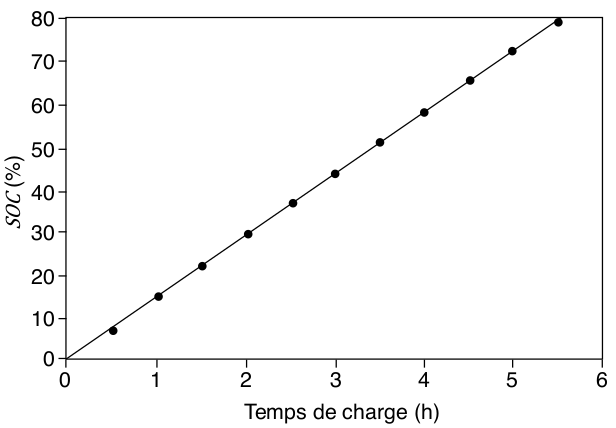
\includegraphics[width=6cm]{figures-Chp0/10-SoC.png}
\end{minipage}\hfill   
\begin{minipage}[c]{0.35\textwidth}     
    \captionof{figure}{\'{E}volution du SoC en fonction du temps de charge.}
    \label{fig:li-ion_car}
\end{minipage}
}

\exercice{
\Q Donner le signe de la puissance et du travail lorsqu'une cellule électrochimique est un récepteur reçoit de l'énergie. Même chose si il s'agit d'un générateur.

Dans les batteries, la puissance électrique est un critère de second plan. Ce qui intéresse principalement les industriels s'est que l'énergie délivrée par la batterie puisse stocker une grande quantité d'énergie, tout en la débitant de manière pérenne dans le temps.

\begin{center}
\begin{adjustbox}{width=0.95\textwidth}
\begin{tabular}{cccccc}
    \toprule
     \textbf{Technologie} & \textbf{Année de développement} & \textbf{Energie massique} & \textbf{Energie volumique} & \textbf{Tension} & \textbf{Cyclabilité}\\
     Unité & & \si{\watt\hour\per\kilo\gram} & \si{\watt\hour\per\liter} & \si{\volt}/au couple \ce{Li^+}/\ce{Li} & $\emptyset$ \\
     \midrule
     Plomb & 1859 & 35 & 70 & 2.0 & 200-250\\
     Nickel-Cadmium & 1900 & 60 & 100 & 1.2 & 400-500\\
     Nickel-Métal-Hydrure & 1975 & 80 & 240 & 1.2 & 400-500\\
     Lithium-Ion & 1978 & 250 & 400 & 3.6 & > 1000\\
     \bottomrule
\end{tabular}   
\end{adjustbox}
\captionof{table}{\small \'{E}volution des ordres de grandeurs de l'énergie massique, volumique, de la tension ainsi que de la cyclabilité d'une batterie en fonction de la technologie.}
\label{tab:battery_time}
\end{center}


\Q Commenter les valeurs de la Tab.\ref{tab:battery_time}. Quel est l'intérêt de la technologie Li-ion par rapport à d'autres technologies ?
\Q Mettre en relation ces données avec la place de l'élément Li au sein du tableau périodique.}

\exercice{
Les batteries utilisées couramment dans les véhicules électriques, mais également dans d'autres applications comme les téléphones portables, sont de type lithium-ion. Elles présentent l'avantage d'avoir une très grande énergie massique, comprise entre 90 et \SI{180}{\watt\hour\per\kilo\gram}. De plus, ces batteries, même partiellement déchargées, délivrent toujours la même puissance, ce qui permet une utilisation dans les mêmes conditions, quel que soit le niveau de charge. Le principe général d'une batterie lithium-ion est basé sur l'échange réversible des ions lithium entre une électrode positive en oxyde métallique (\ce{MO2}) et une électrode négative en graphite qui va stocker les ions lithium pendant la charge :

~

\begin{minipage}[c]{0.65\textwidth}
\centering
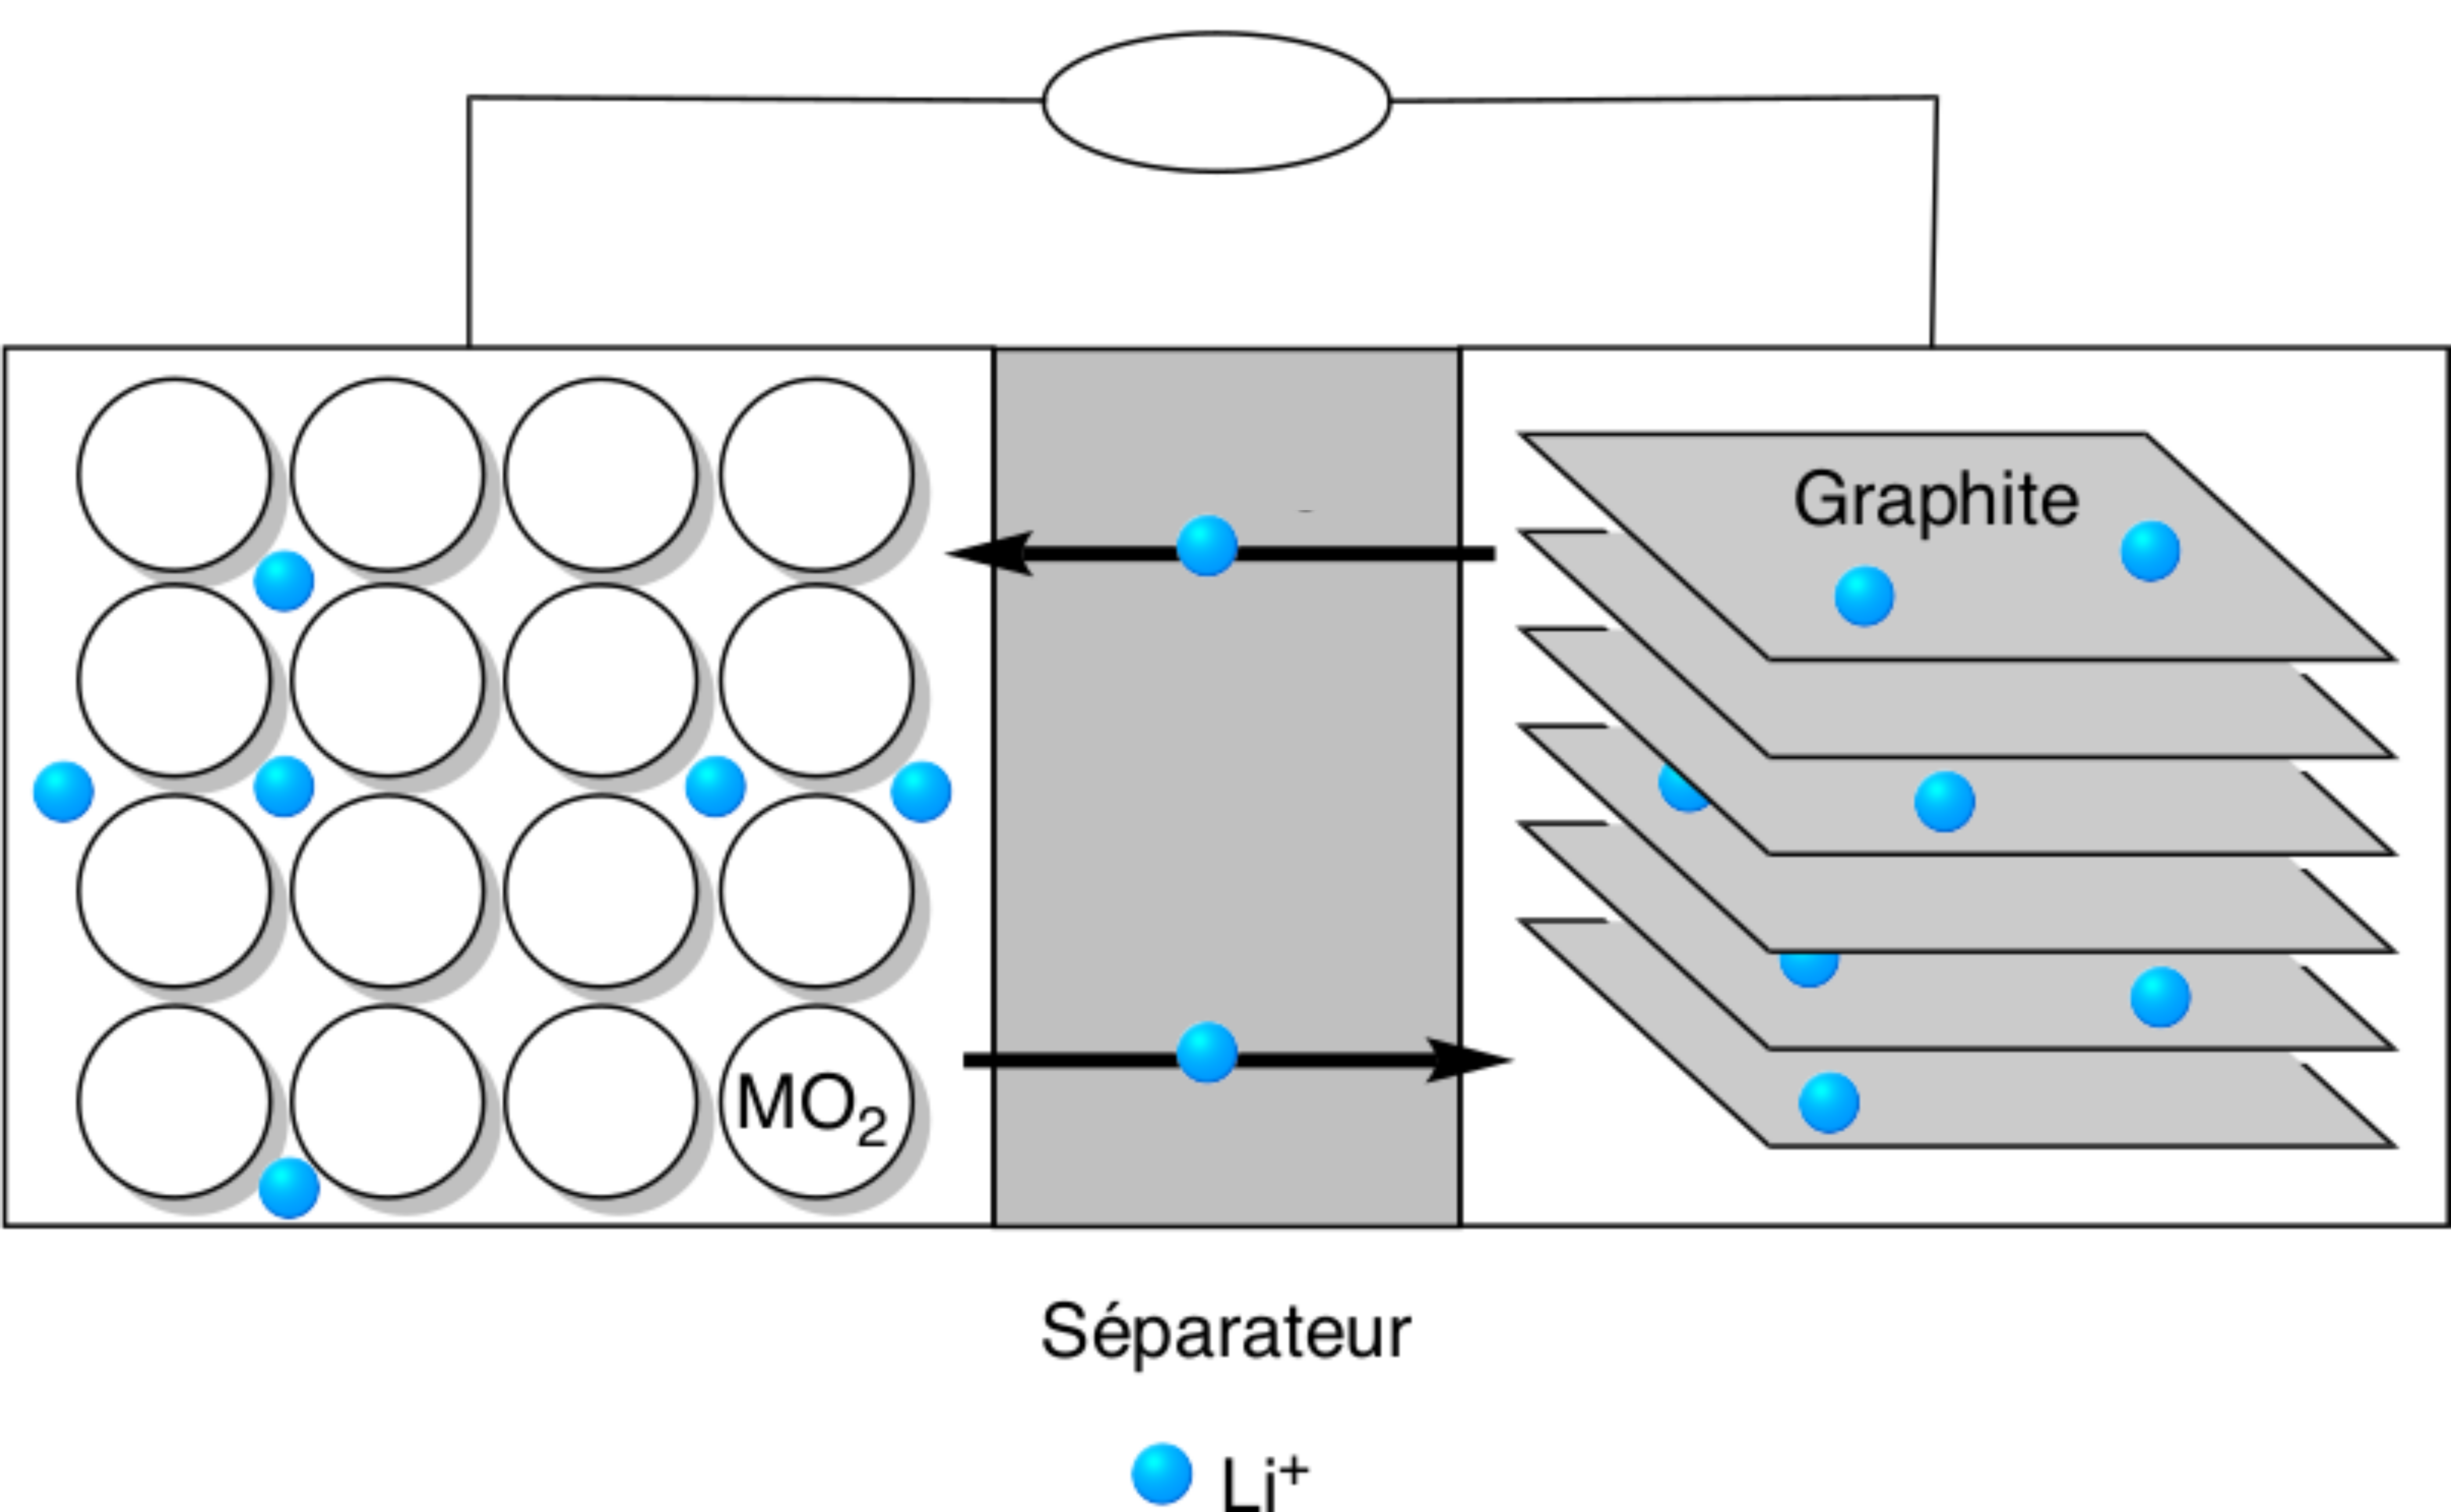
\includegraphics[width=6cm]{figures-Chp0/7-BatteryLithium.png}
\end{minipage}\hfill   
\begin{minipage}[c]{0.35\textwidth}     
\captionof{figure}{Technologie au lithium-ion. Le solvant utilisé est une espèce organique.}
\label{fig:li-ion}
\end{minipage}

\Q En vous appuyant sur la représentation du graphite, expliqué pourquoi les ions Li peuvent s'insérer entre les feuillets de graphite. On sait que le rayon ionique du lithium est de \SI{60}{\pico\meter} et le covalent est de \SI{134}{\pico\meter}.

\begin{minipage}[c]{0.65\textwidth}
\centering
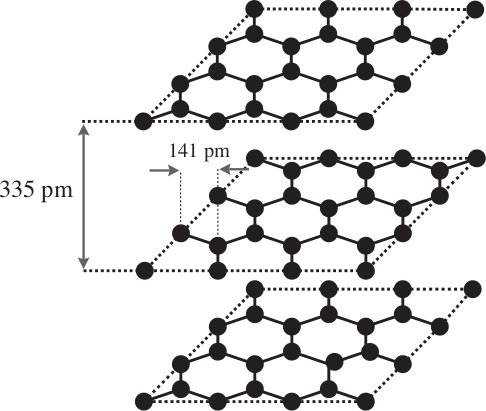
\includegraphics[height=4cm]{figures-Chp0/11-graphene.png}
\end{minipage}\hfill   
\begin{minipage}[c]{0.35\textwidth}     
\centering
\captionof{figure}{Structure du graphite}
\label{fig:graphite}
\end{minipage}

\Q A l'état totalement chargé, la structure du composé est \ce{LiC6}. Écrire la demi-équation rédox à cette électrode lors de la charge et de la décharge et préciser le signe de l'électrode de graphite.
La seconde électrode peut être en oxyde de cobalt (\ce{CoO2}) qui, après insertion des ions lithium,
forme l'oxyde lithié \ce{LiCoO2}. 
\Q Montrer que c'est l'élément cobalt qui change de degré d'oxydation ;
\Q Donner la demi-équation électronique associée au couple considéré lors de la charge et de la décharge
à cette électrode en précisant son signe.
\Q Reproduire et orienter le schéma de la Fig. \ref{fig:li-ion} dans le cas d'une charge puis d'une décharge. Vous indiquerez le nom et le signe des électrodes puis le flux d'électron, le courant électrique et la direction de migration des ions lithium.
%tiré de Mines-Pont 2022.

~

La suite de cet exercice sera traité à la partie suivante.}
\end{comment}